\subsection{External Interface Requirements}

\subsubsection{User Interfaces}
% In this section we present user interfaces for Students and Educators. 
% \begin{center}
%     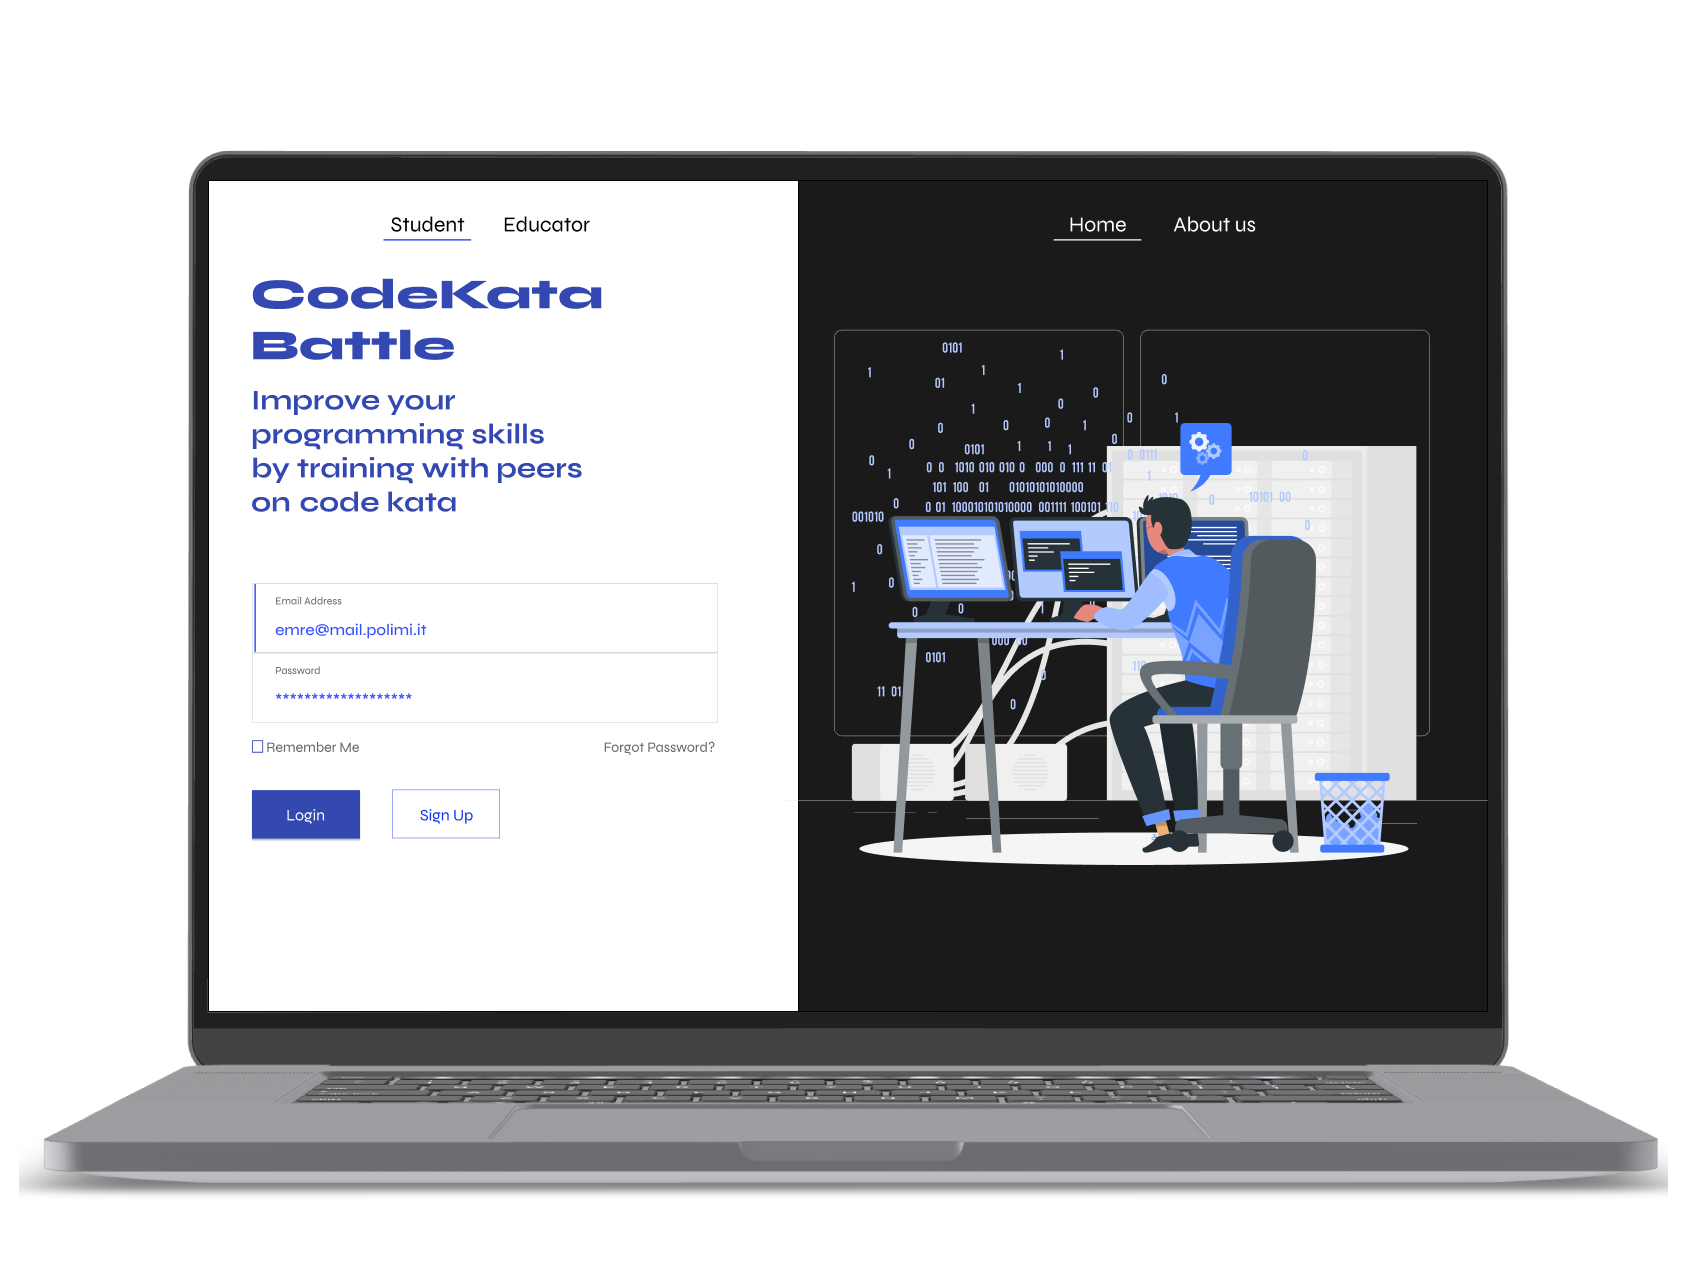
\includegraphics[scale=0.13]{Images/ui-ux/login-signup/student_login.png}
%     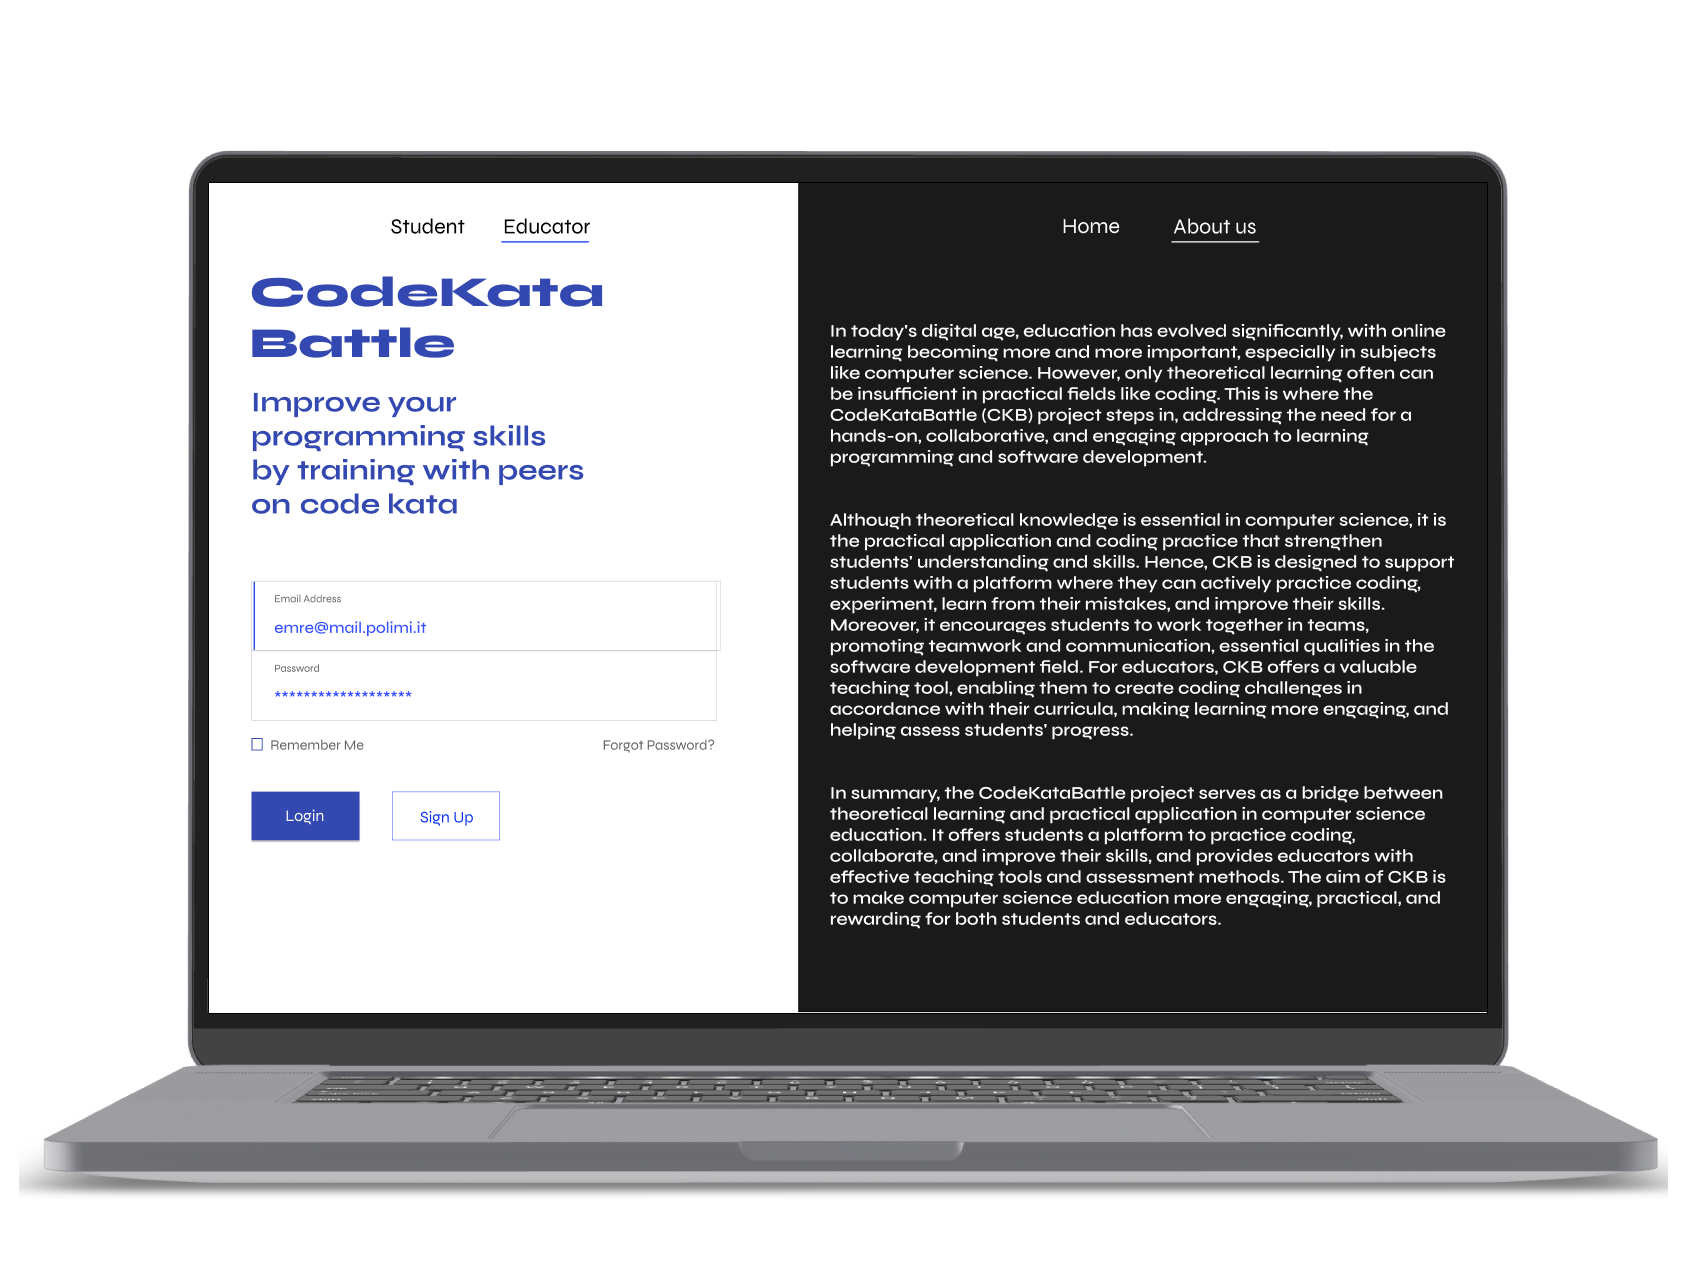
\includegraphics[scale=0.13]{Images/ui-ux/login-signup/educator_login.png}
% \end{center}
%     \begin{center}
%         (a) Login Screens
%     \end{center}
% \begin{center}
%     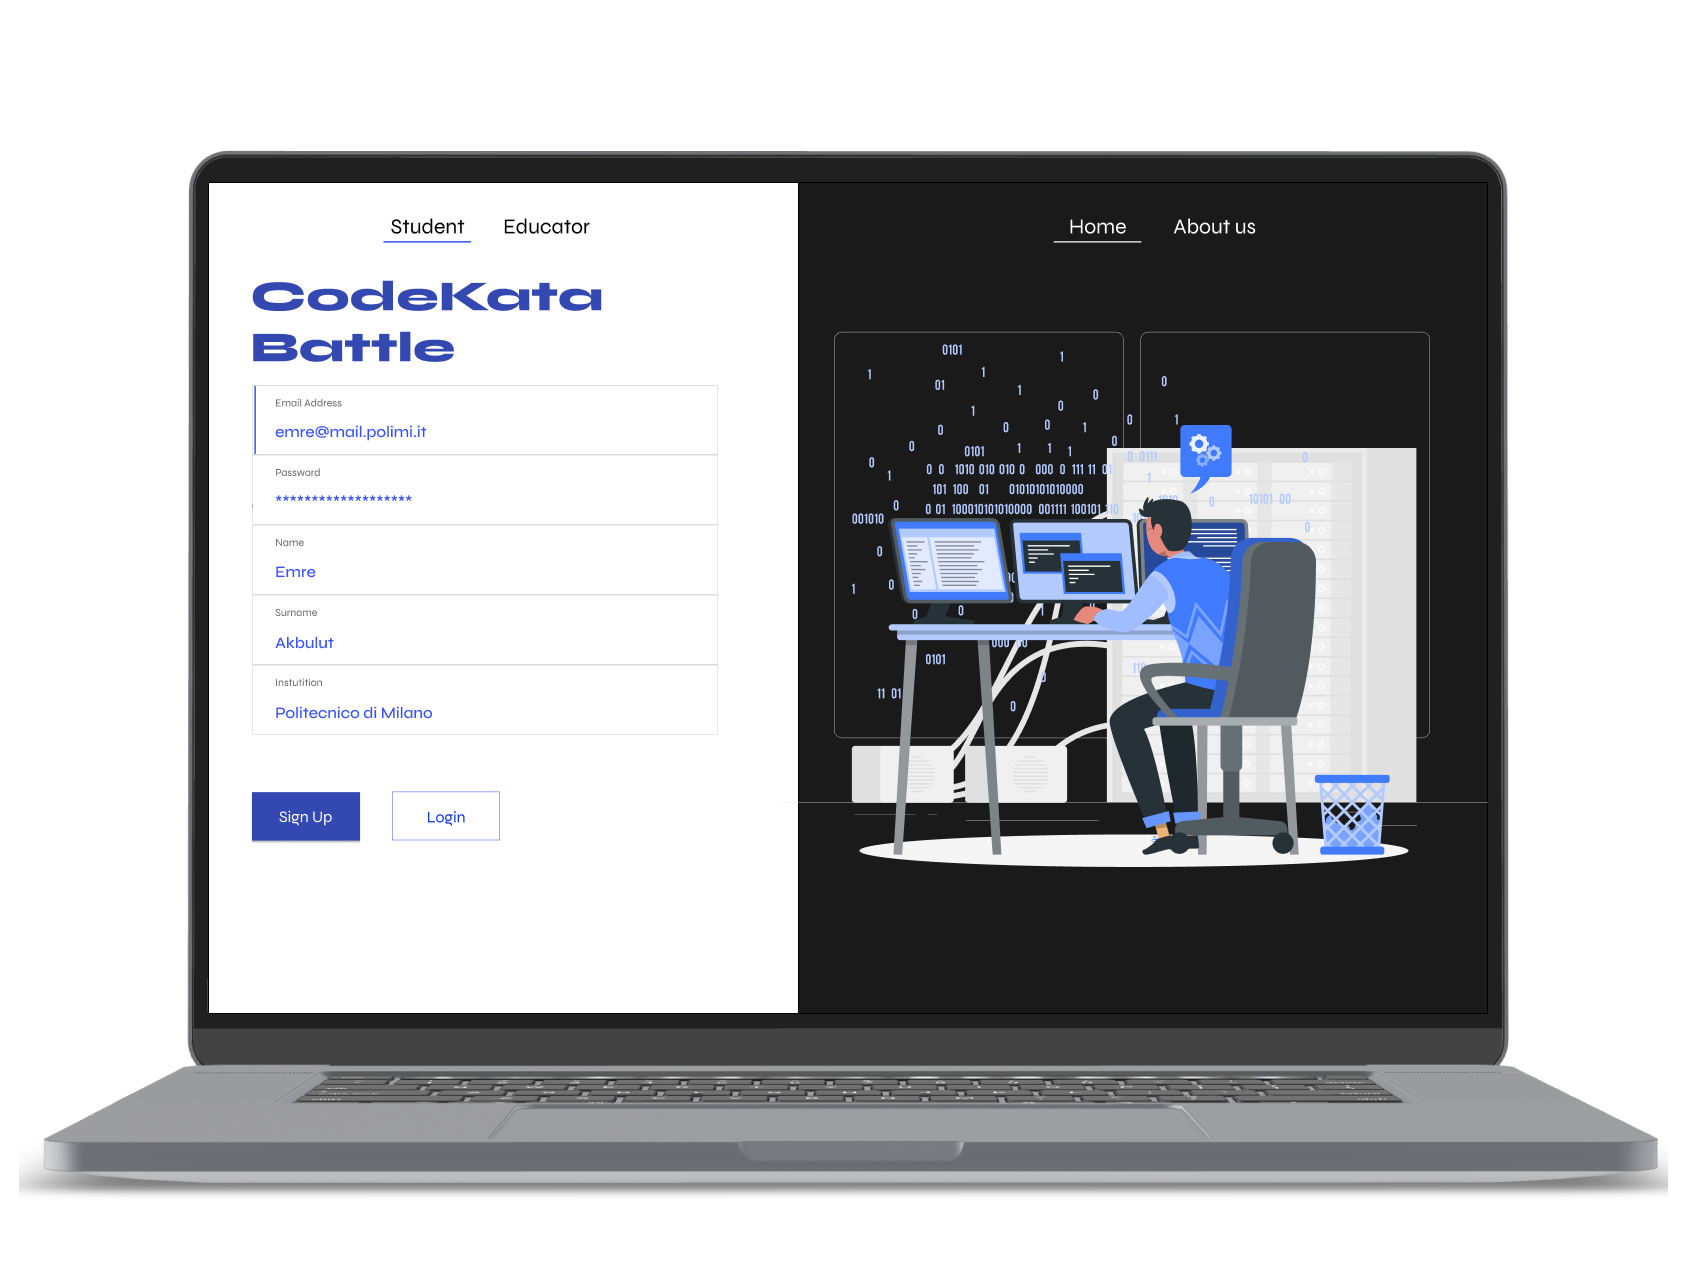
\includegraphics[scale=0.13]{Images/ui-ux/login-signup/student_signup.png}
%     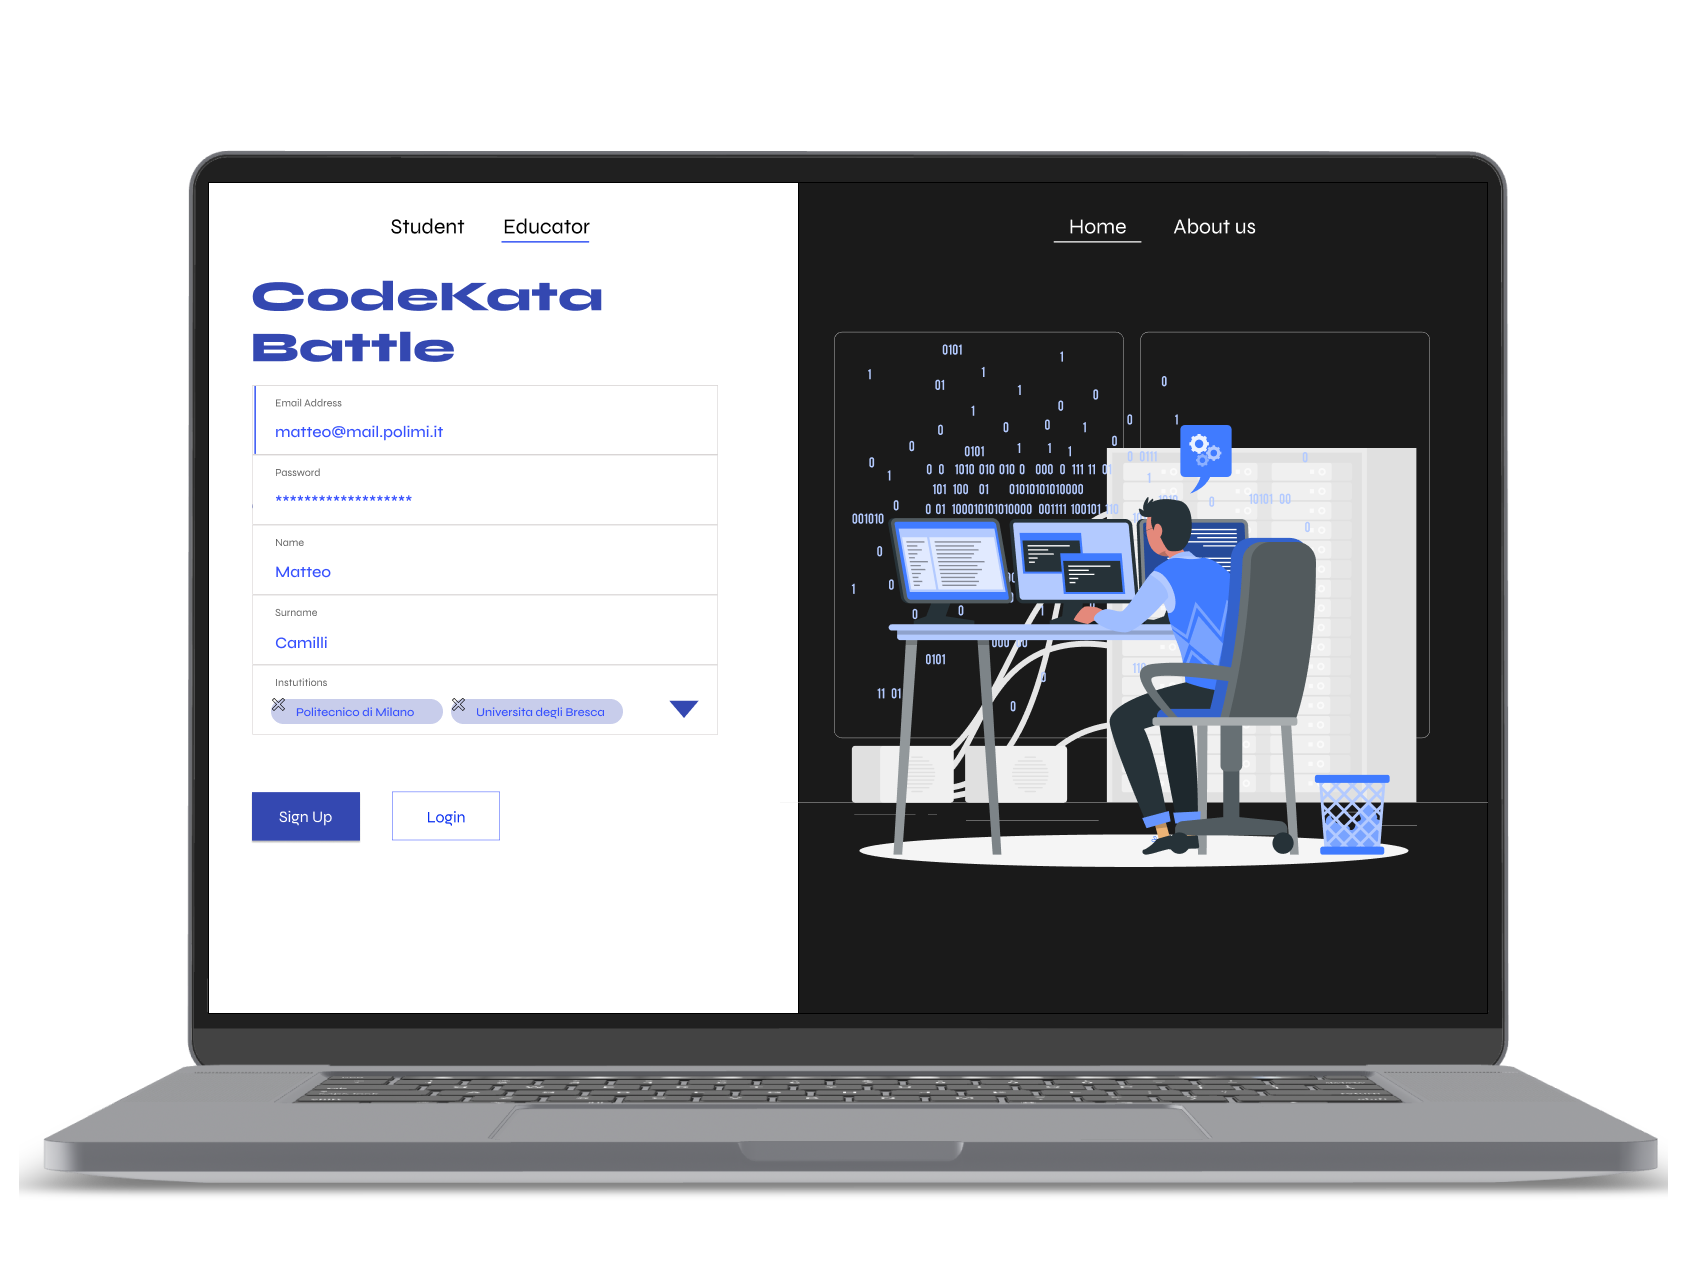
\includegraphics[scale=0.13]{Images/ui-ux/login-signup/educator_signup.png}
%     (a) Sign up Screens
% \end{center}
% \newpage
% \begin{center}
%     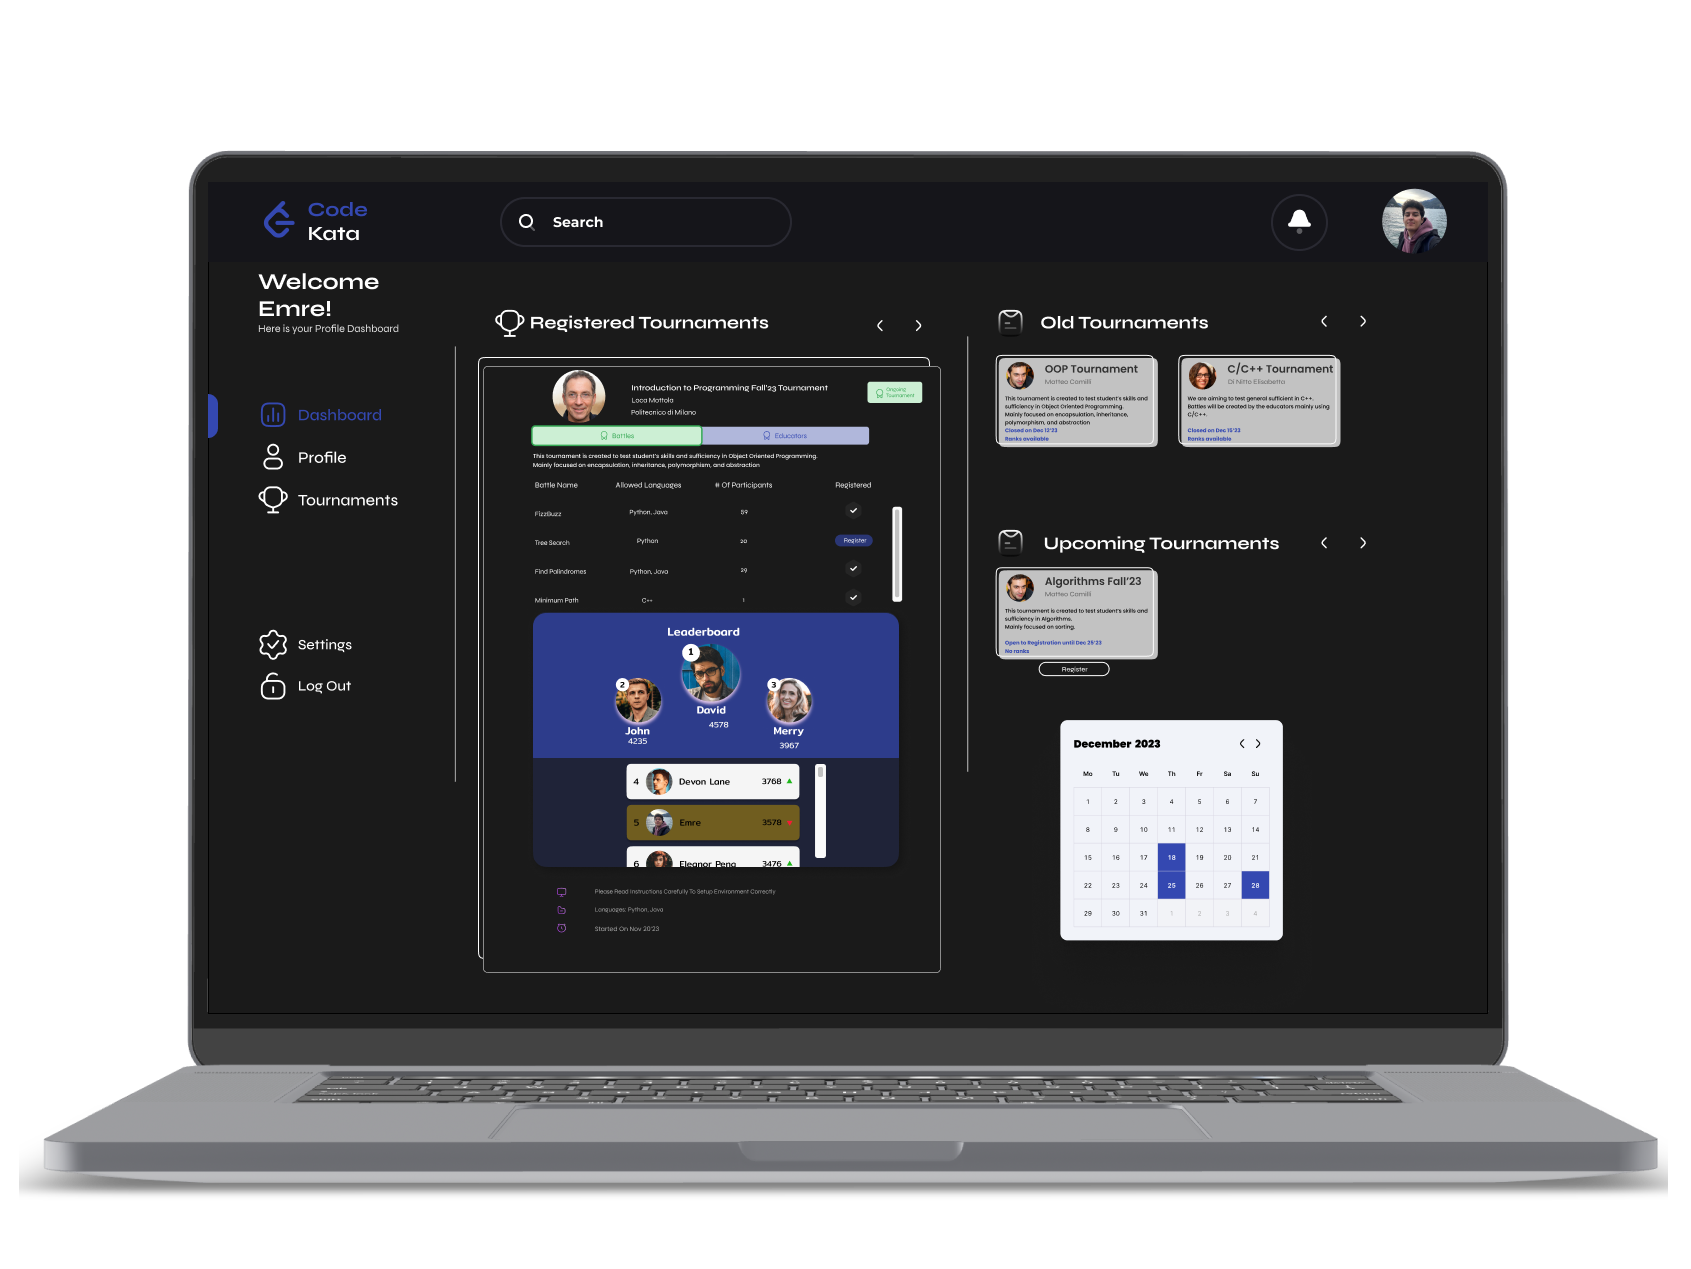
\includegraphics[scale=0.13]{Images/ui-ux/student_dashboard/student_dashboard_1.png}
%     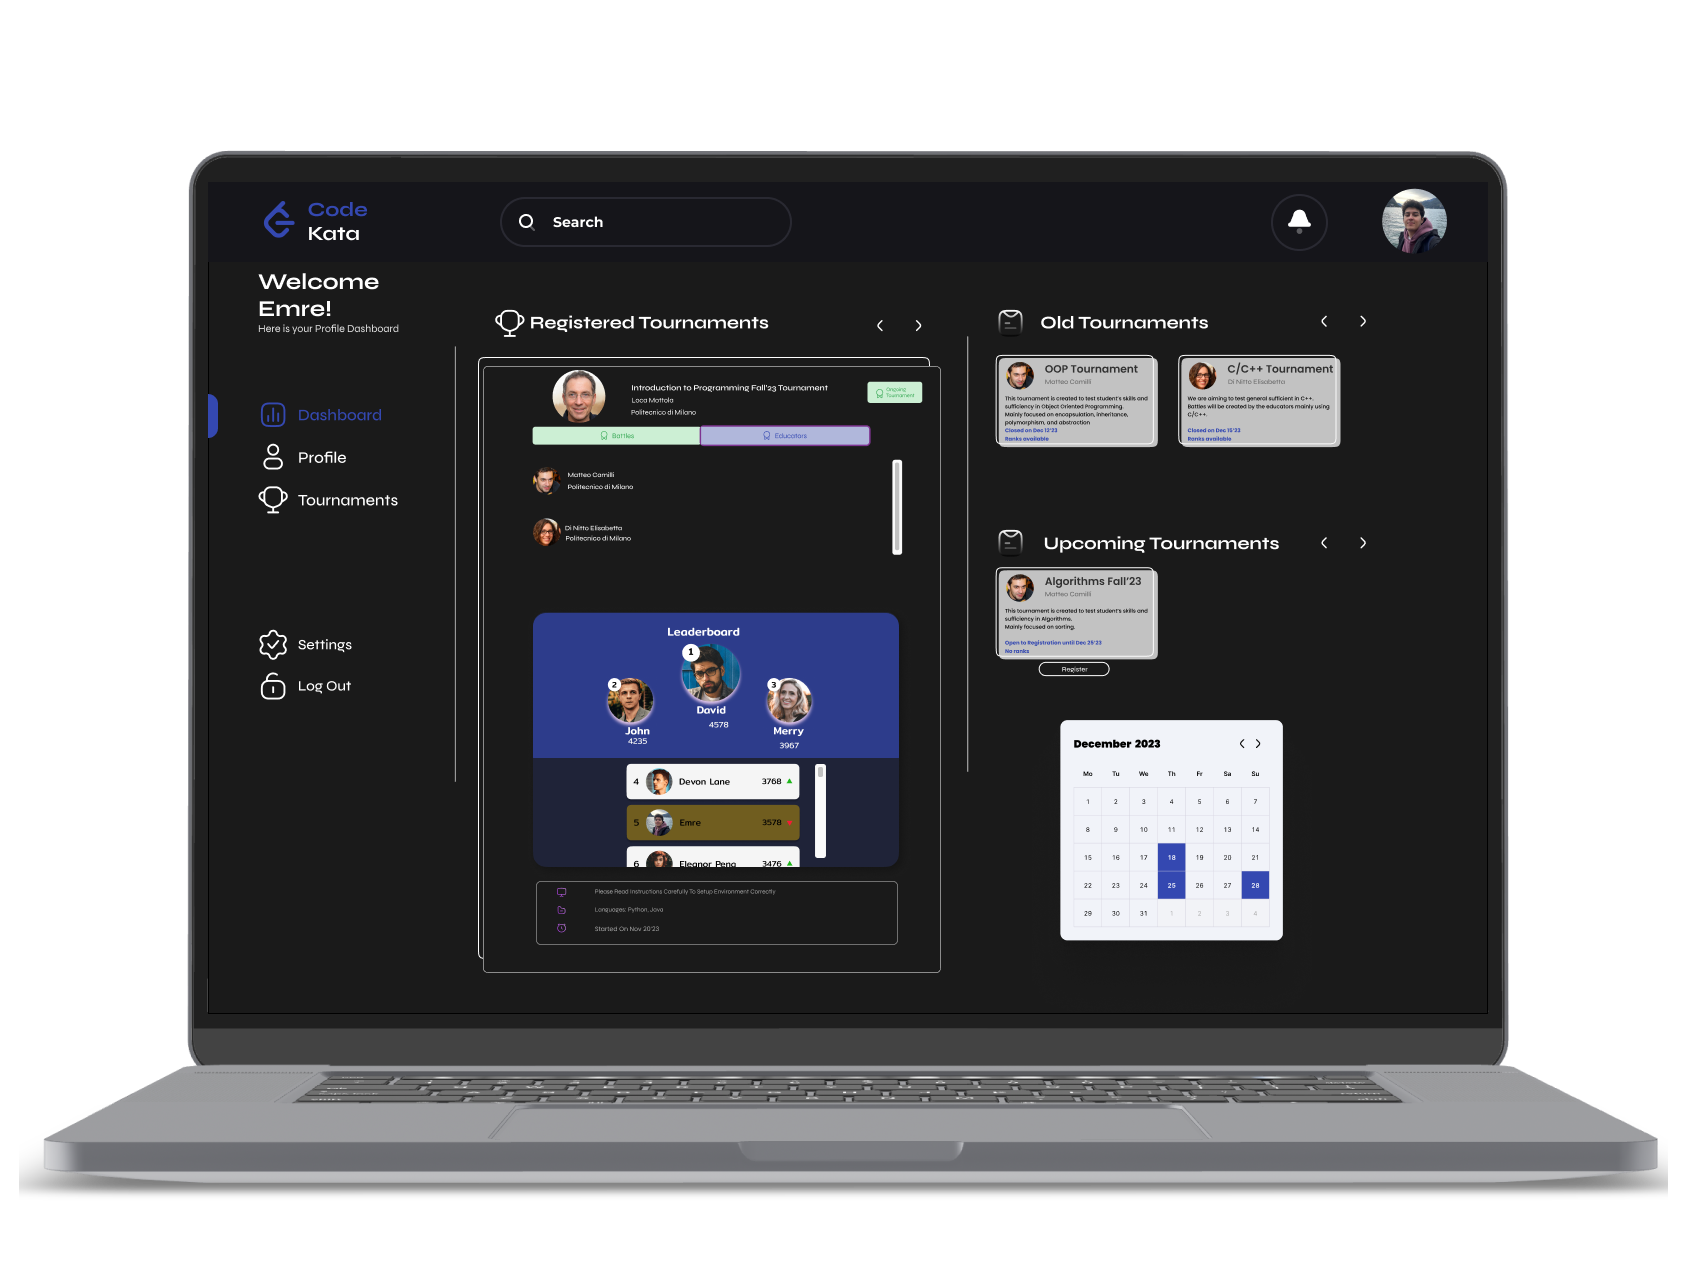
\includegraphics[scale=0.13]{Images/ui-ux/student_dashboard/student_dashboard_2.png}
%             (a) Student Dashboard
% \end{center}
% \begin{center}
%     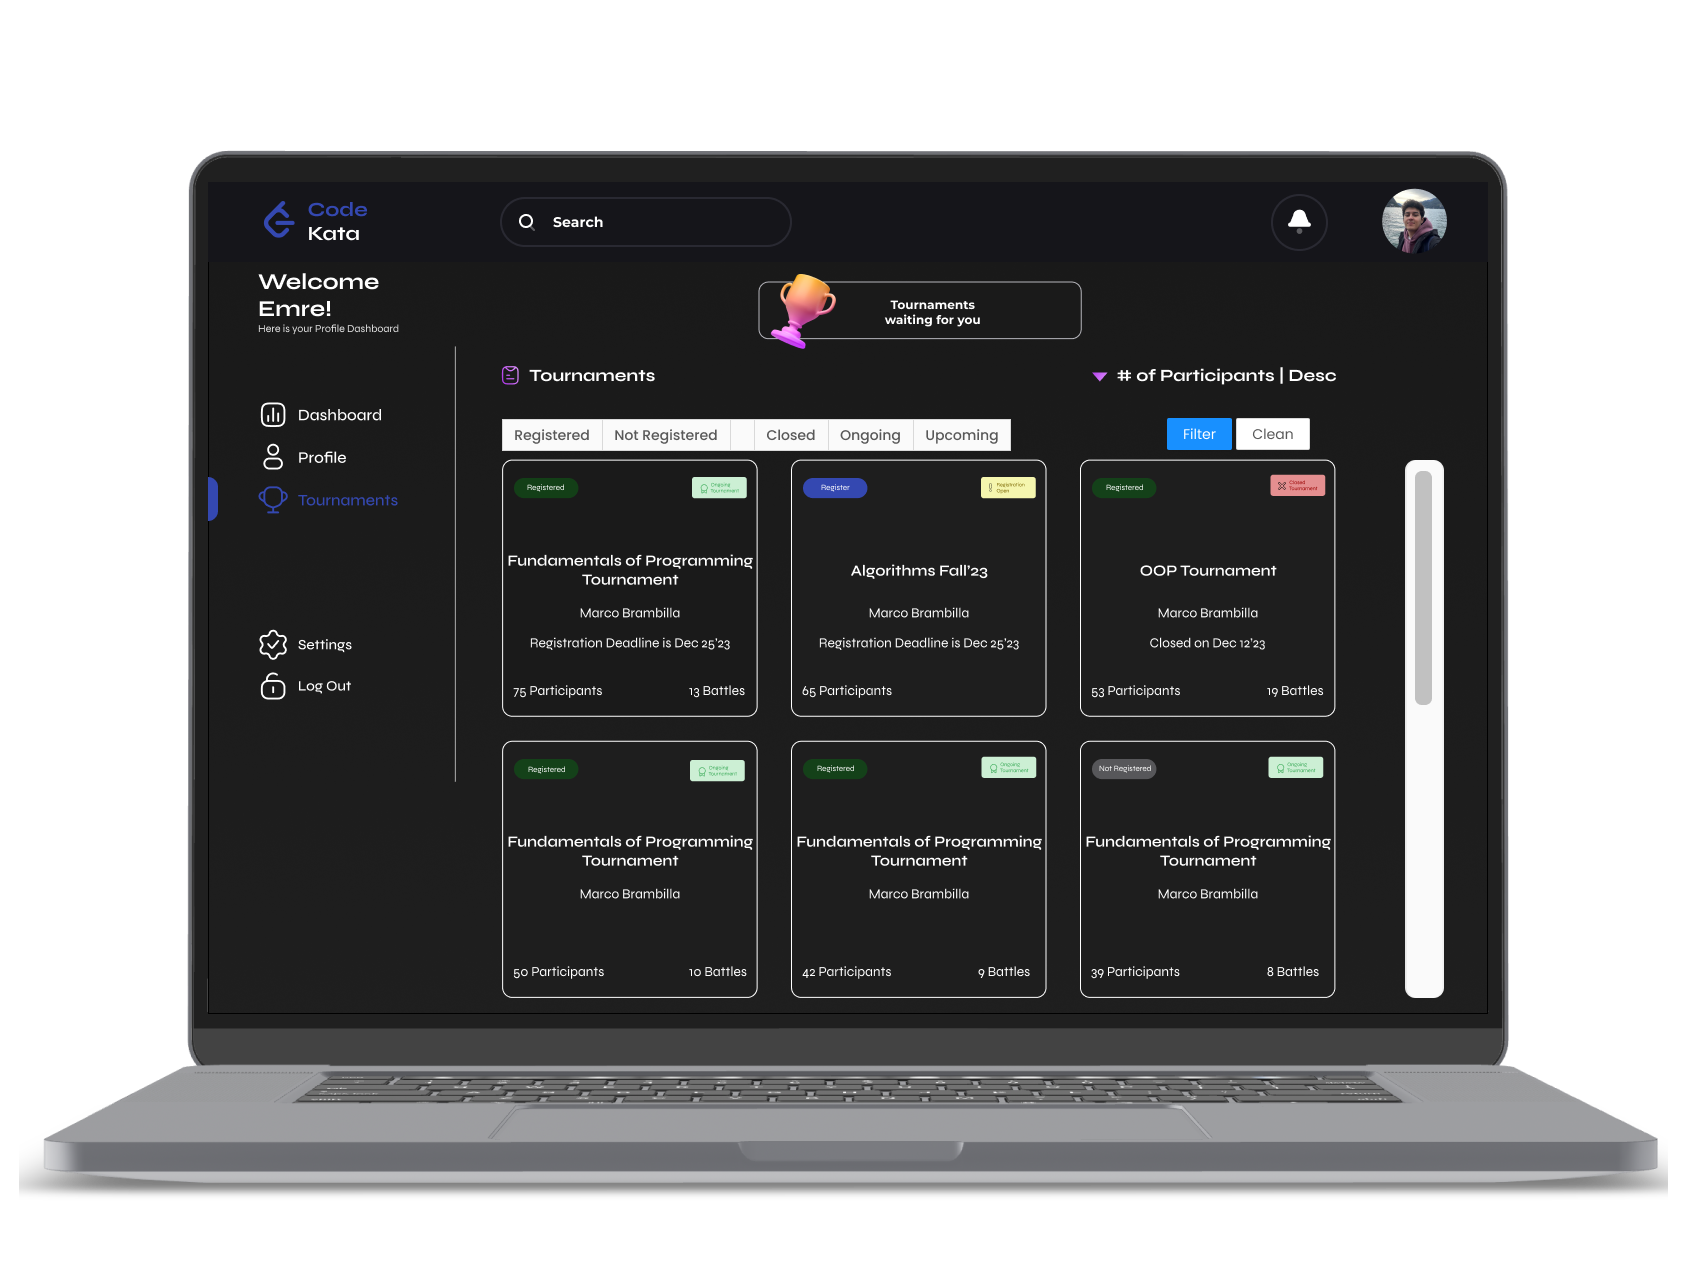
\includegraphics[scale=0.13]{Images/ui-ux/student_tournaments/student_tournaments_1.png}
%     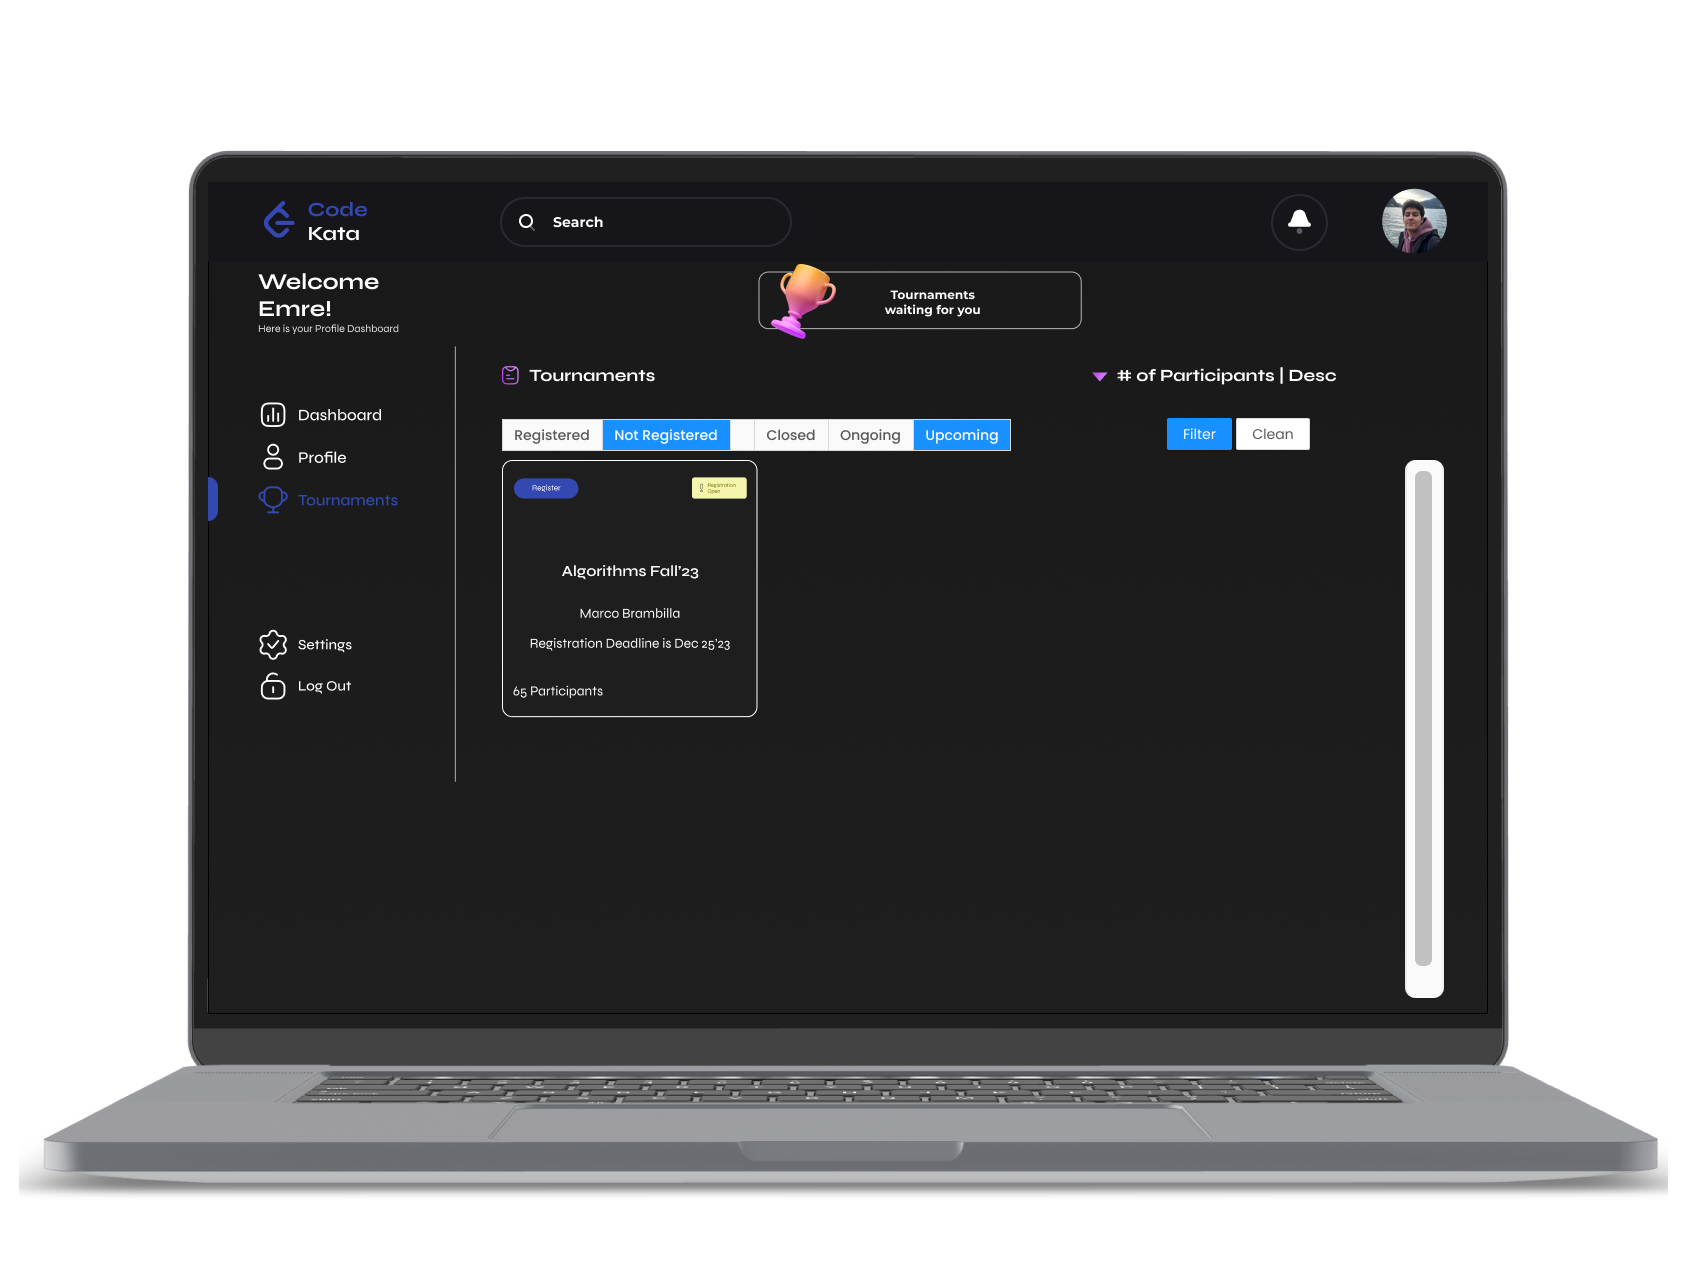
\includegraphics[scale=0.13]{Images/ui-ux/student_tournaments/student_tournaments_2.png}    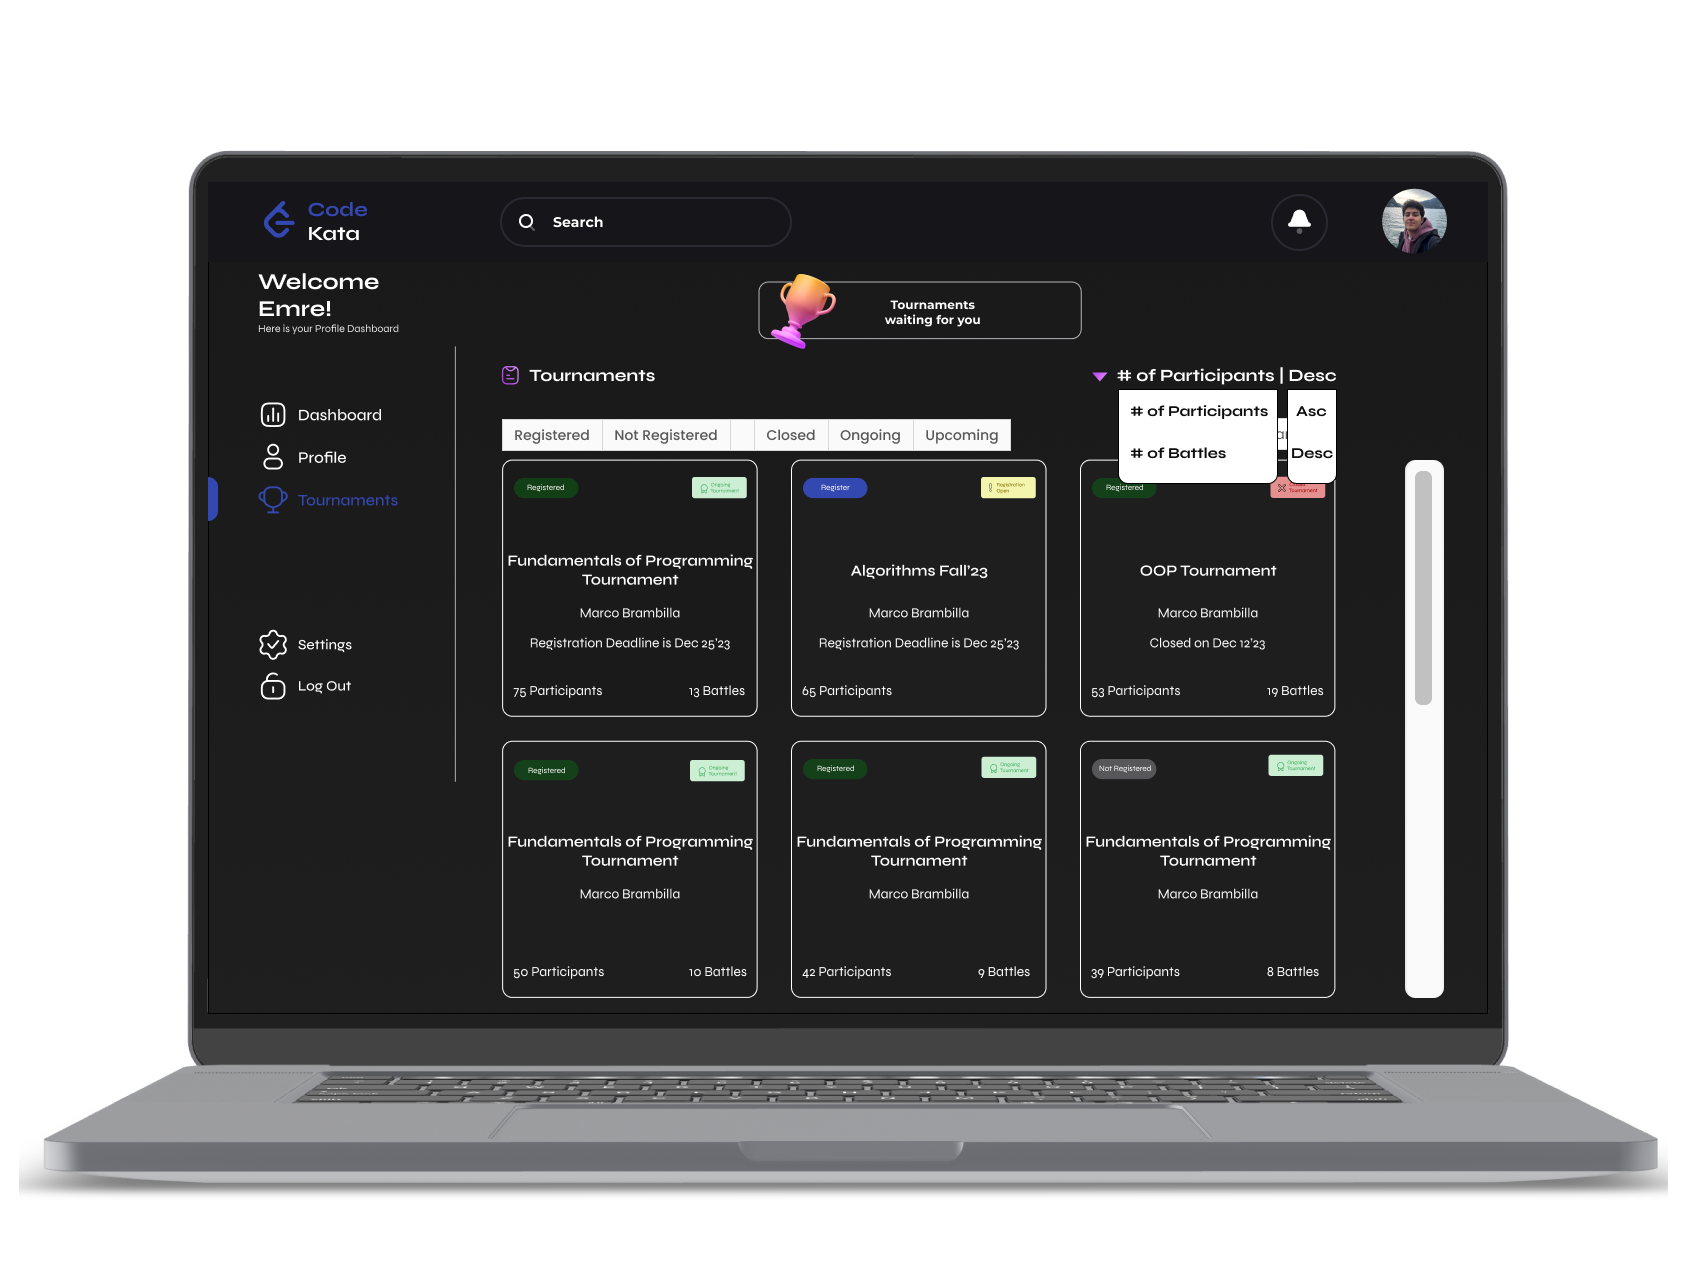
\includegraphics[scale=0.13]{Images/ui-ux/student_tournaments/student_tournaments_3.png}    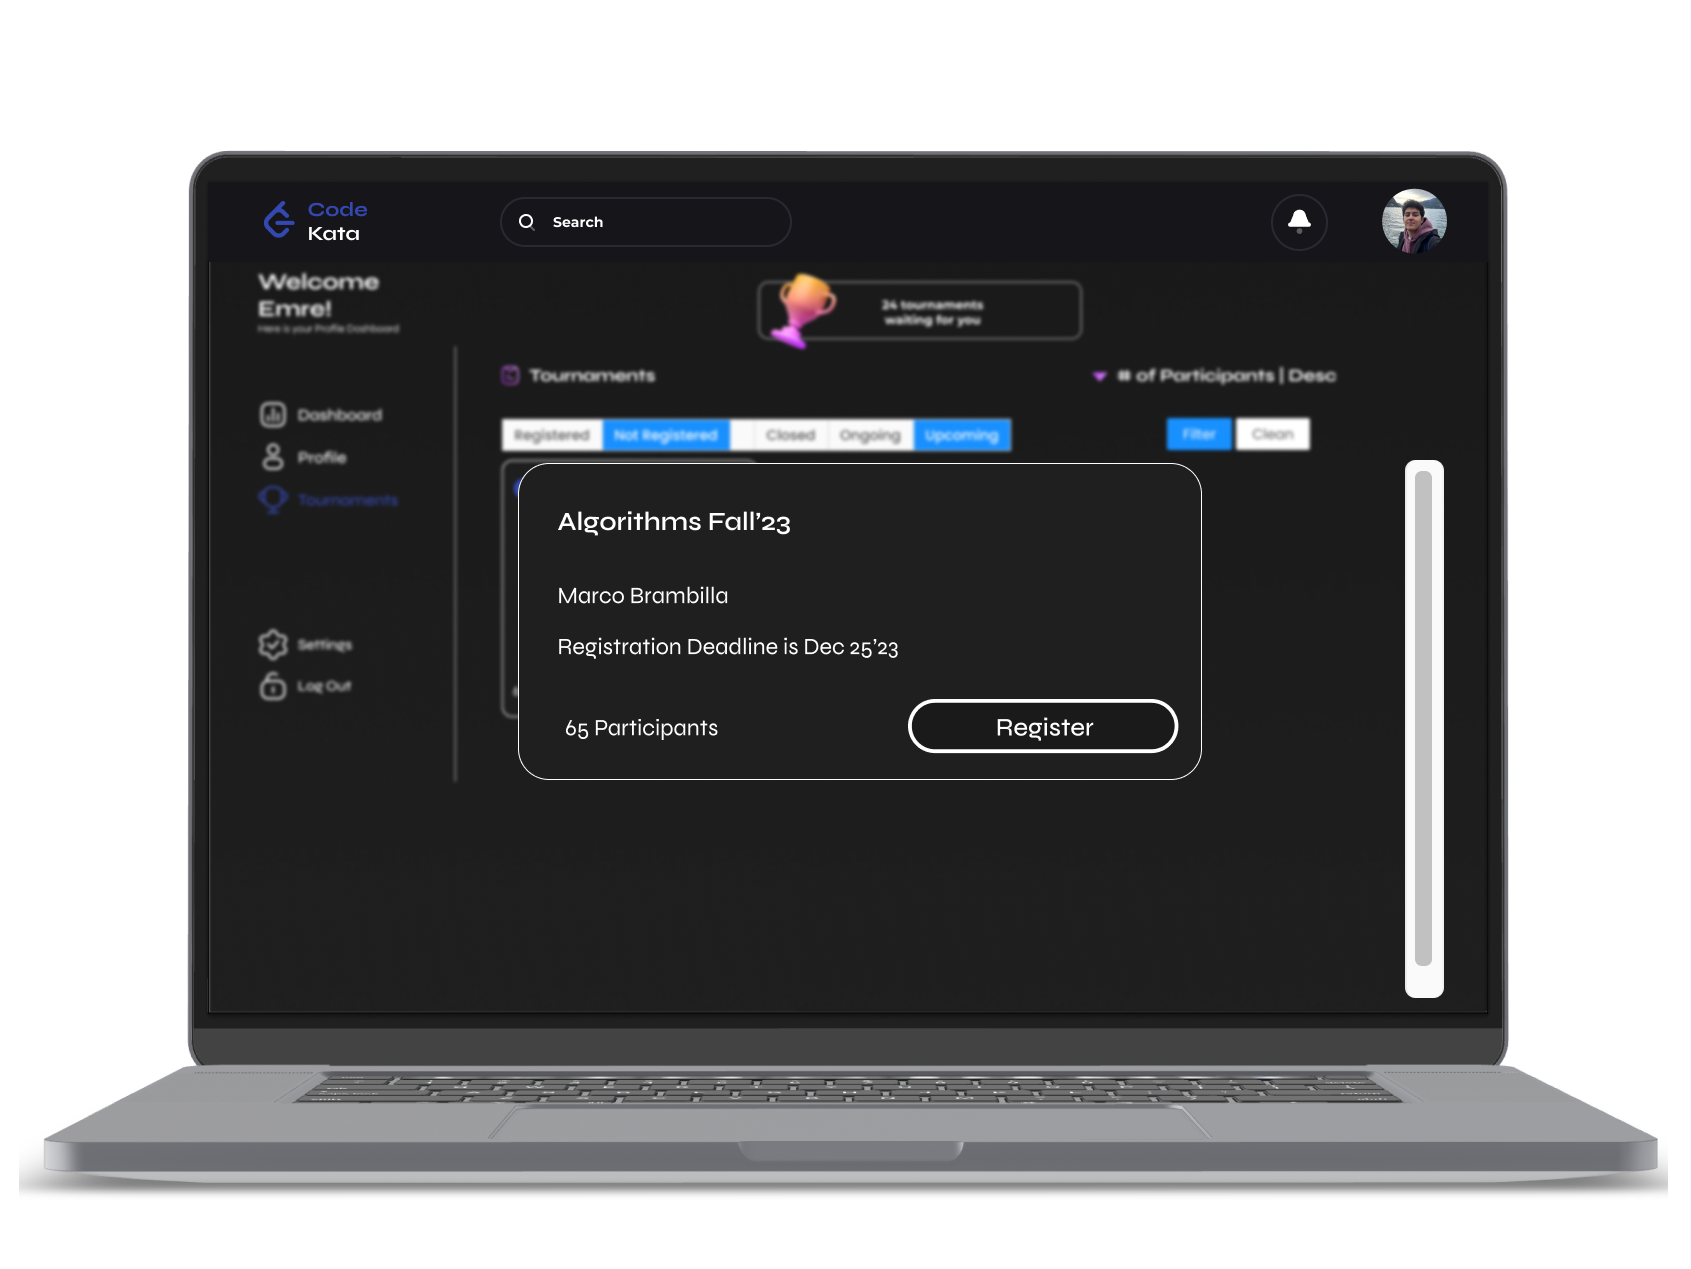
\includegraphics[scale=0.13]{Images/ui-ux/student_tournaments/student_tournaments_4.png}
%         (a) Student Tournaments
% \end{center}

% \begin{center}
%     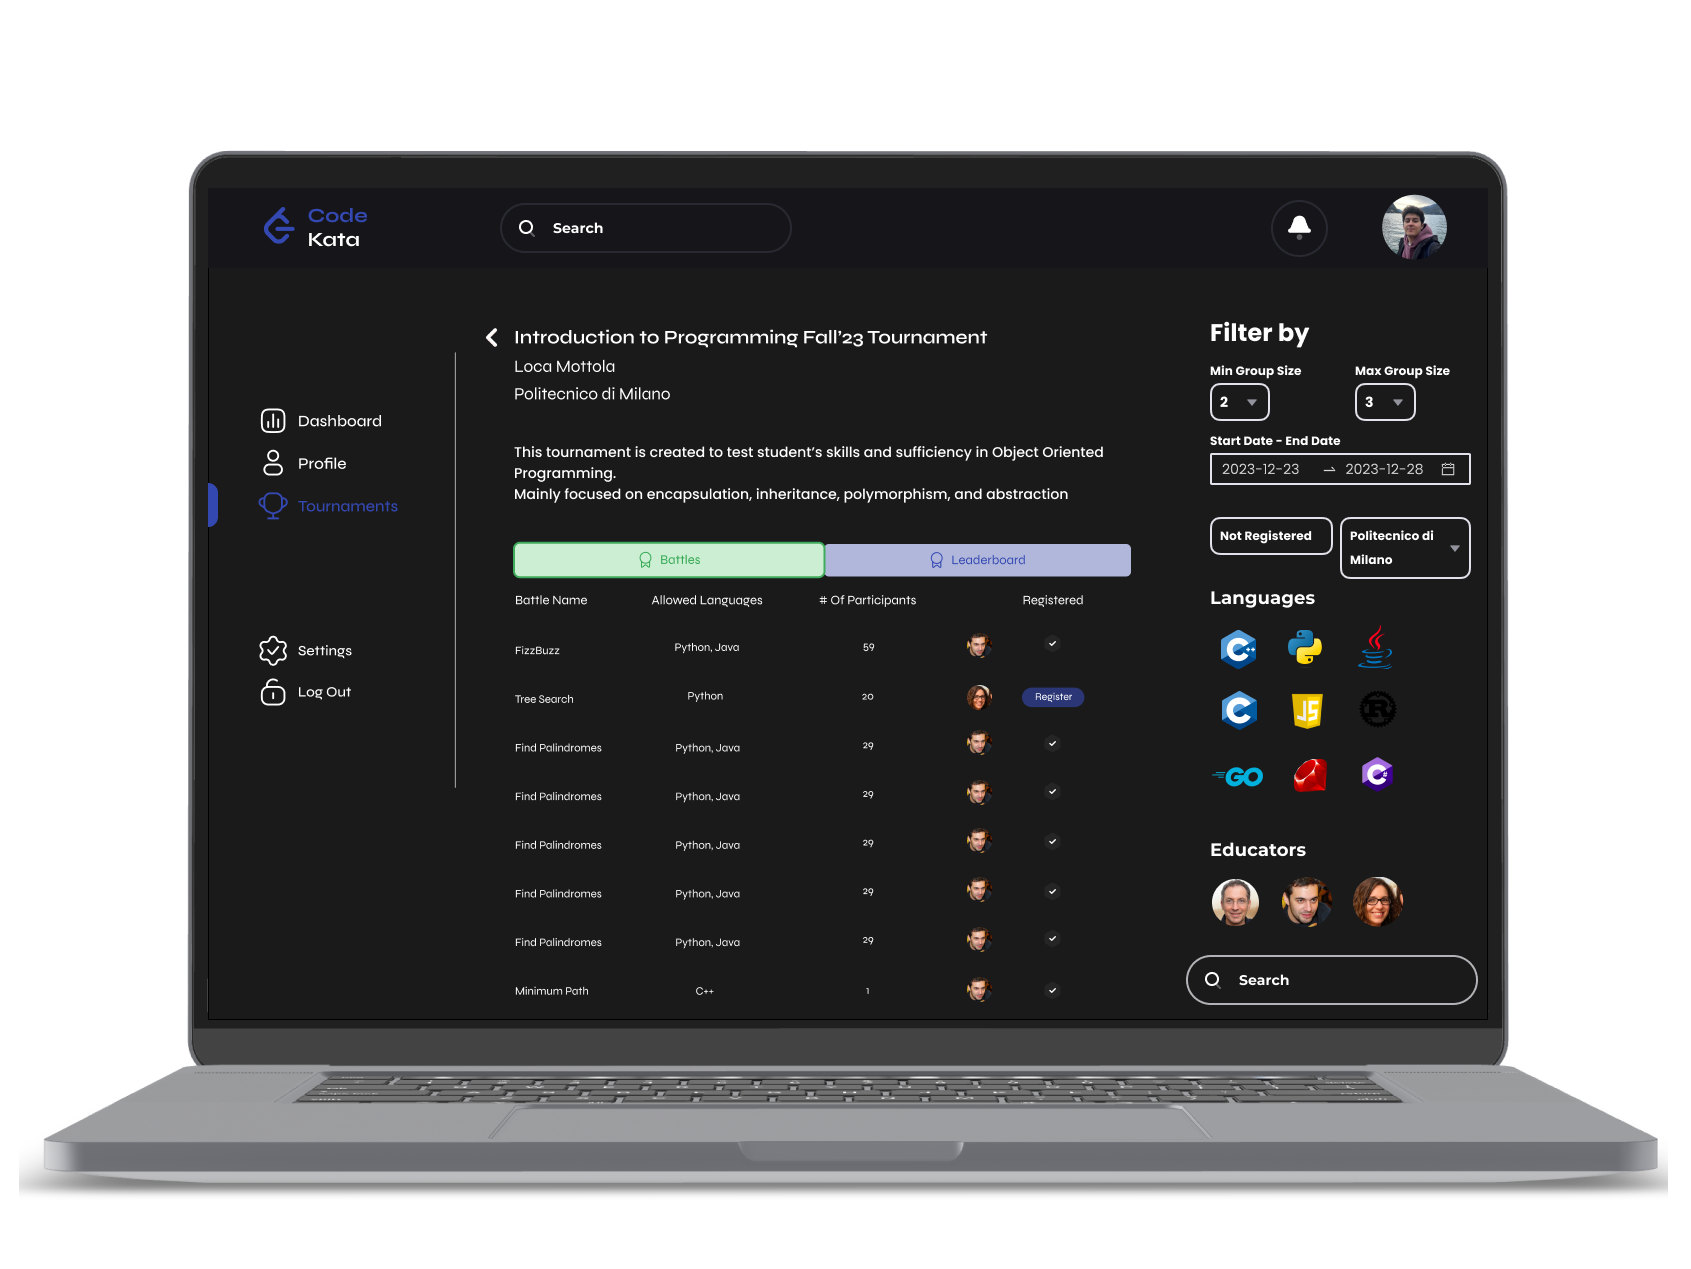
\includegraphics[scale=0.13]{Images/ui-ux/student_tournament/student_tournament_1.png}
%     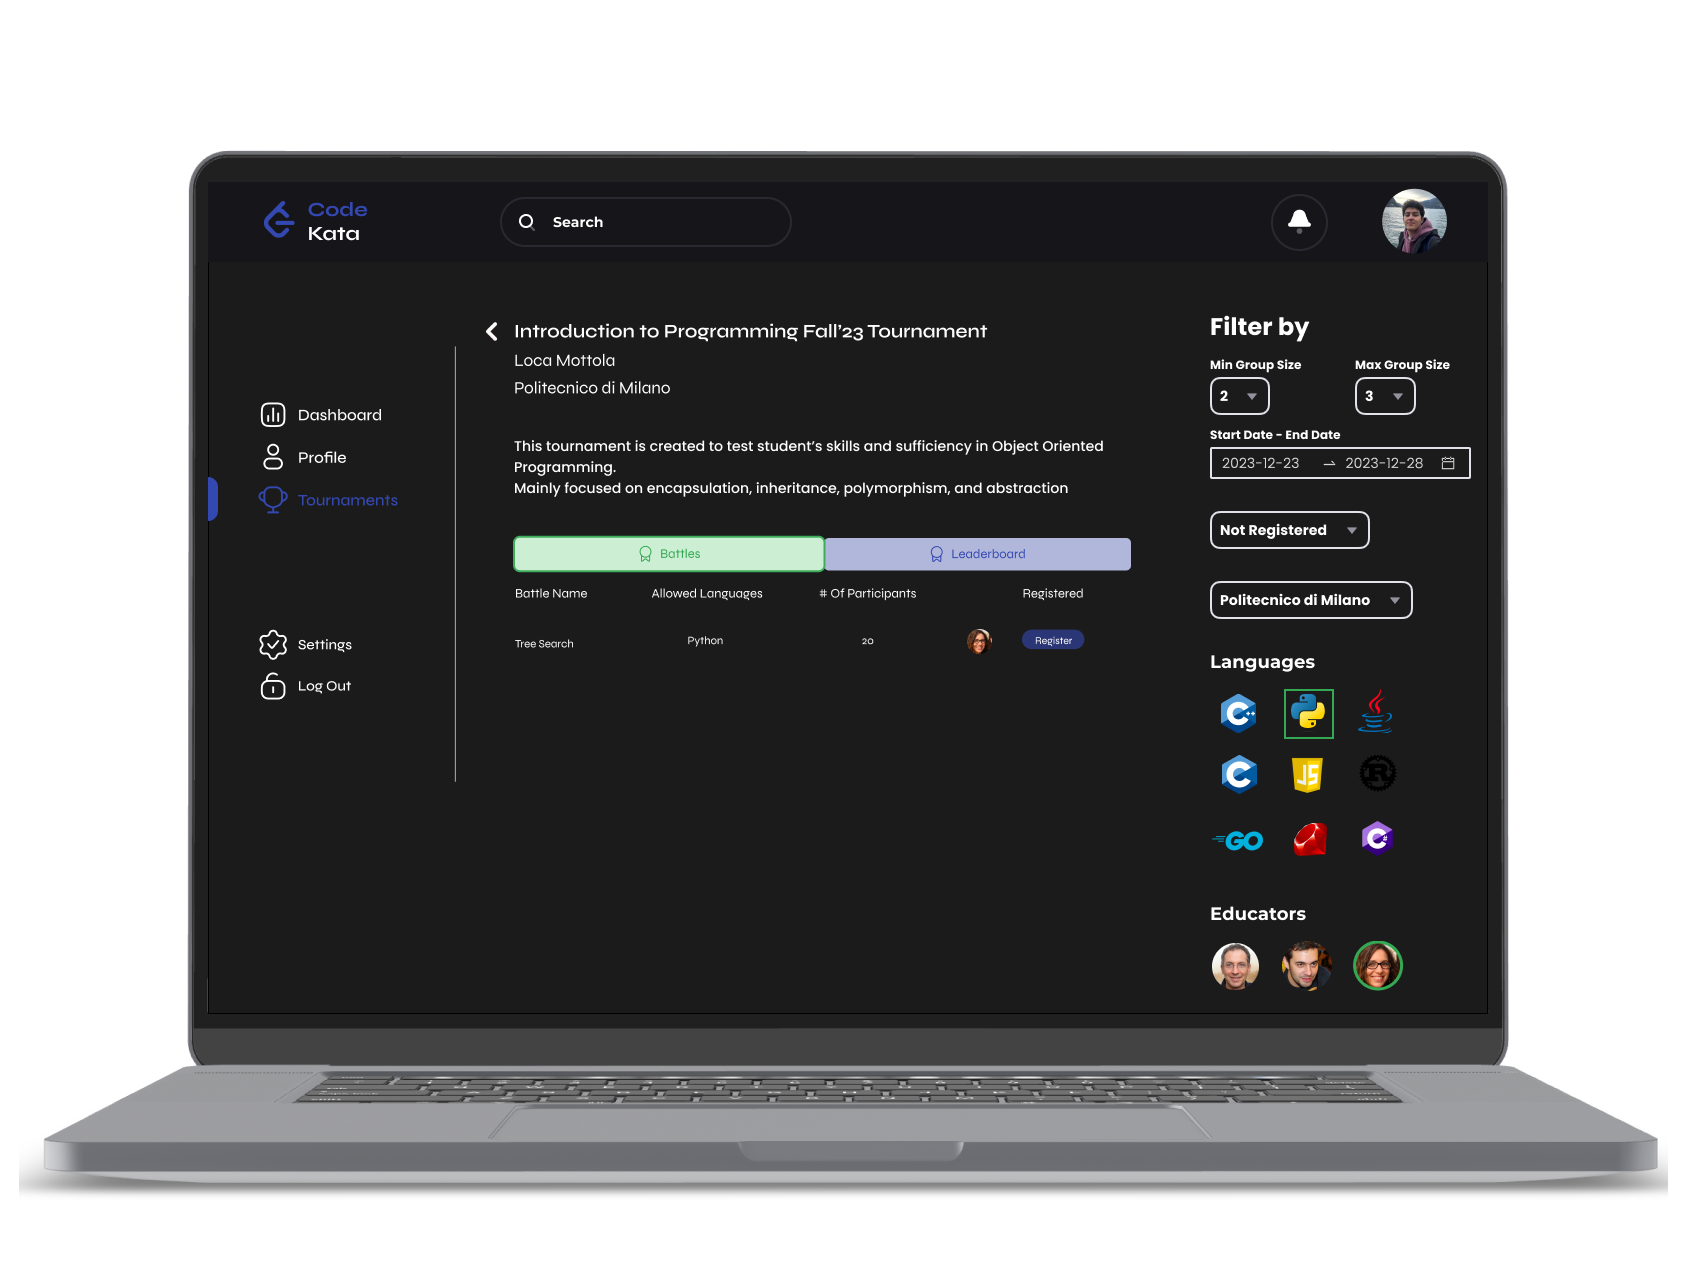
\includegraphics[scale=0.13]{Images/ui-ux/student_tournament/student_tournament_2.png}    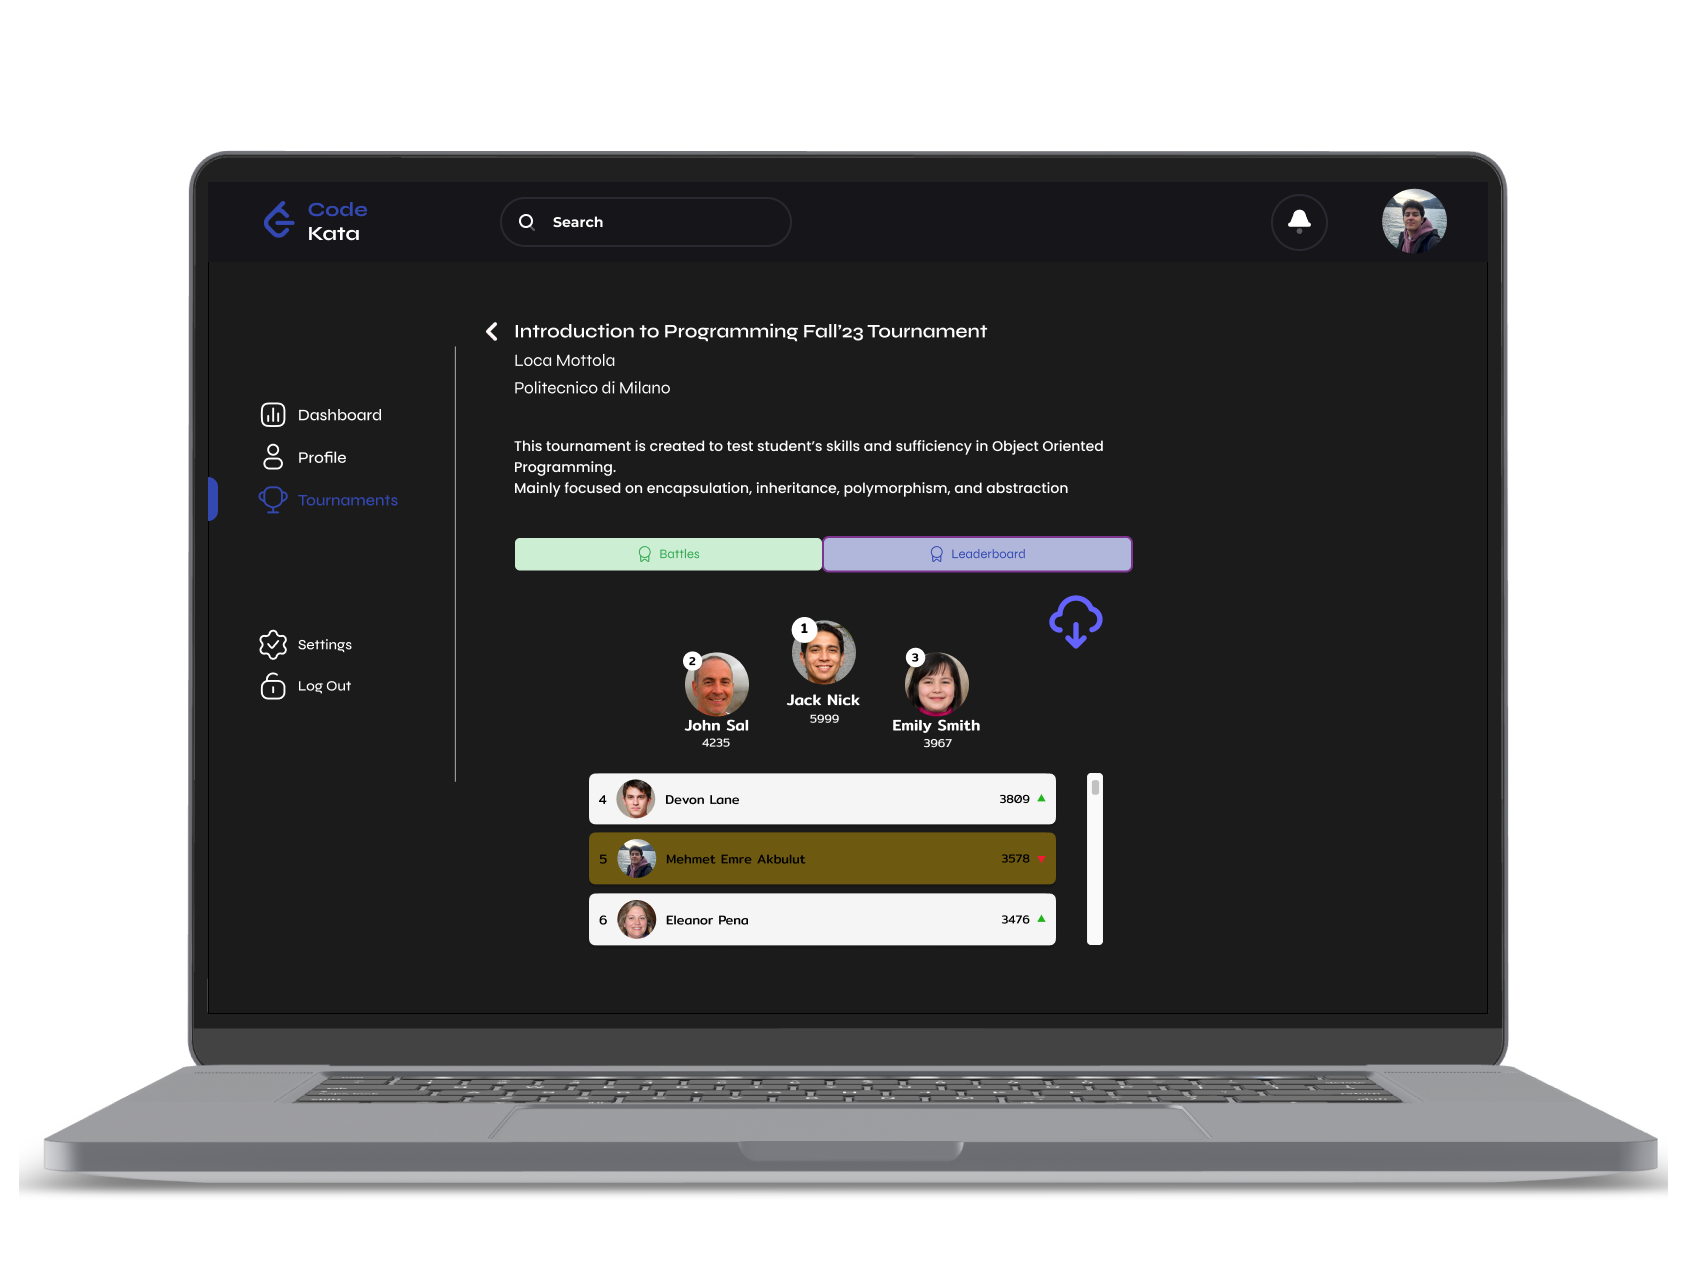
\includegraphics[scale=0.13]{Images/ui-ux/student_tournament/student_tournament_3.png} 
%     \\ (a) Student and A Tournament
% \end{center}
% \newpage
% \begin{center}
% 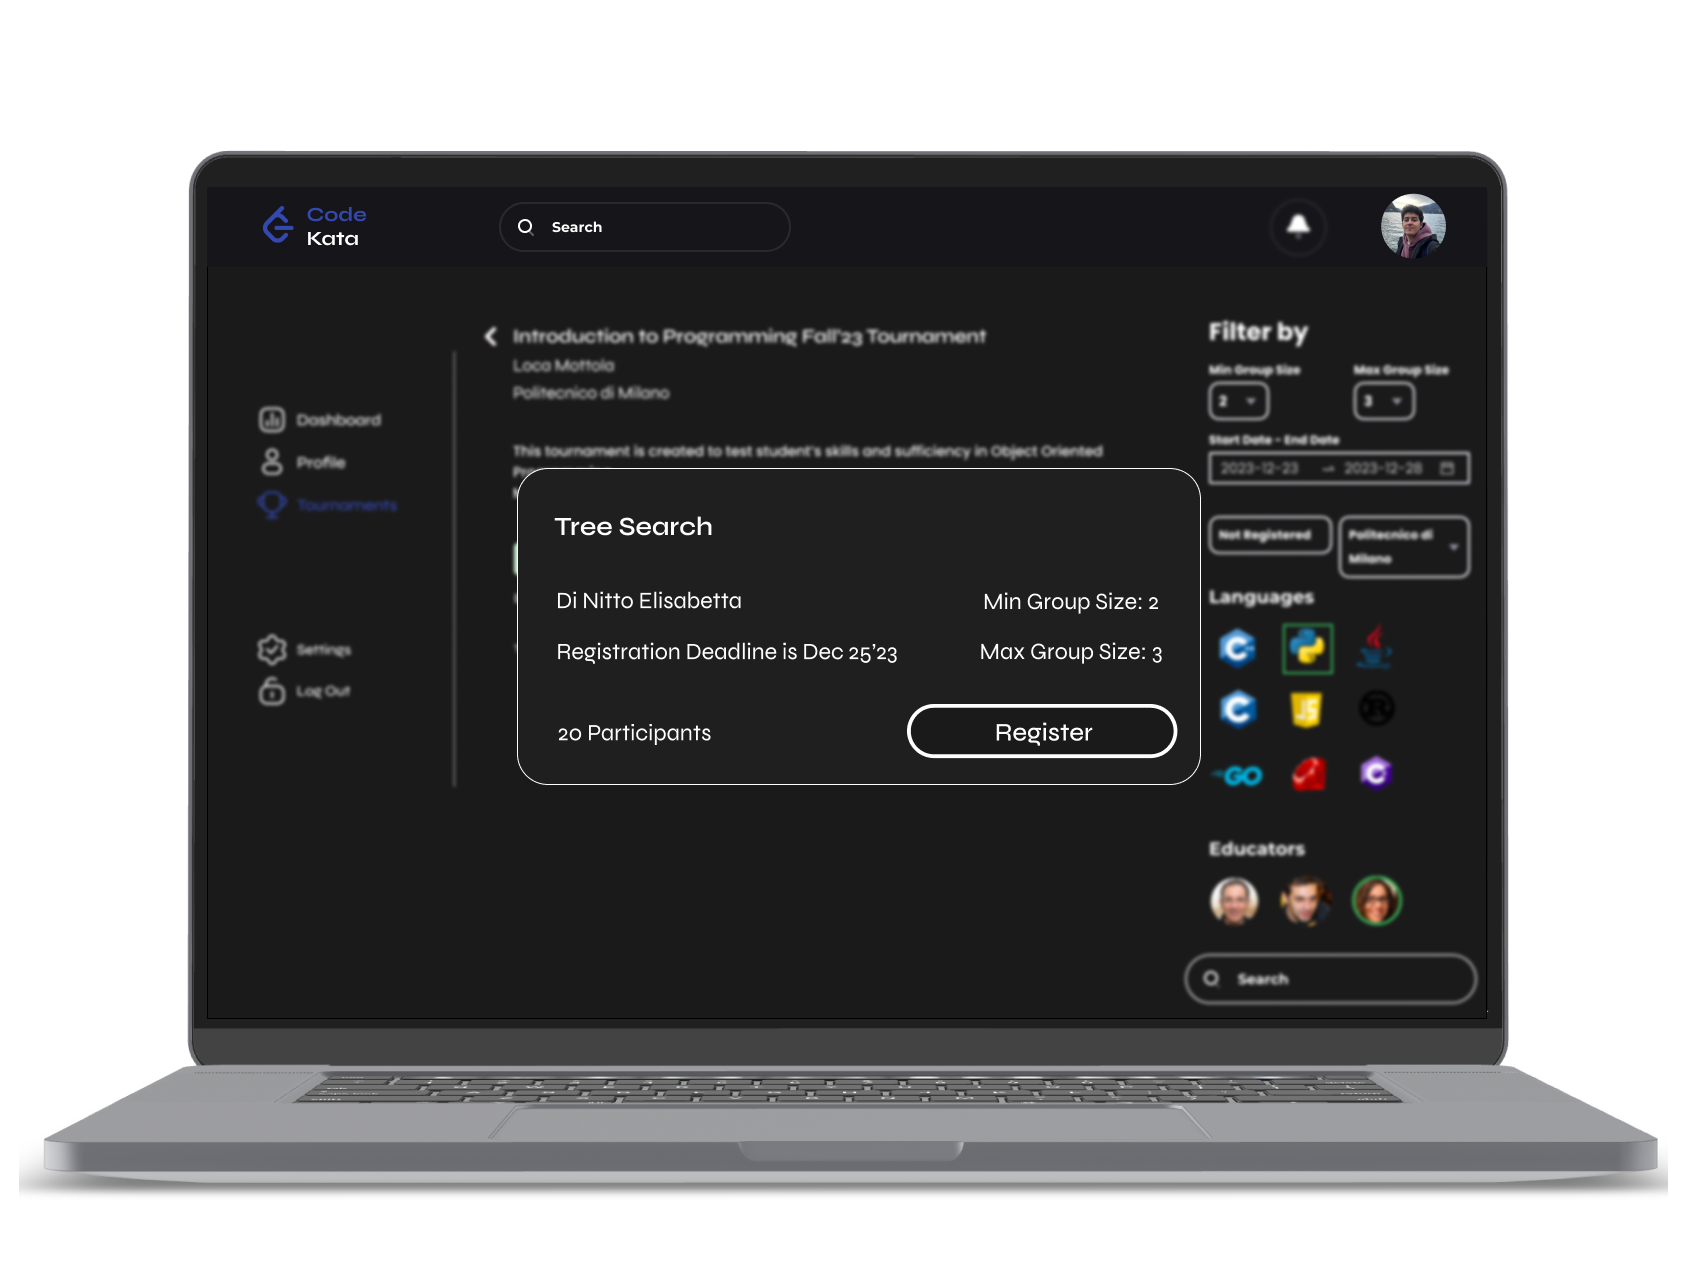
\includegraphics[scale=0.13]{Images/ui-ux/student_battle_register/student_battle_register_1.png}
% 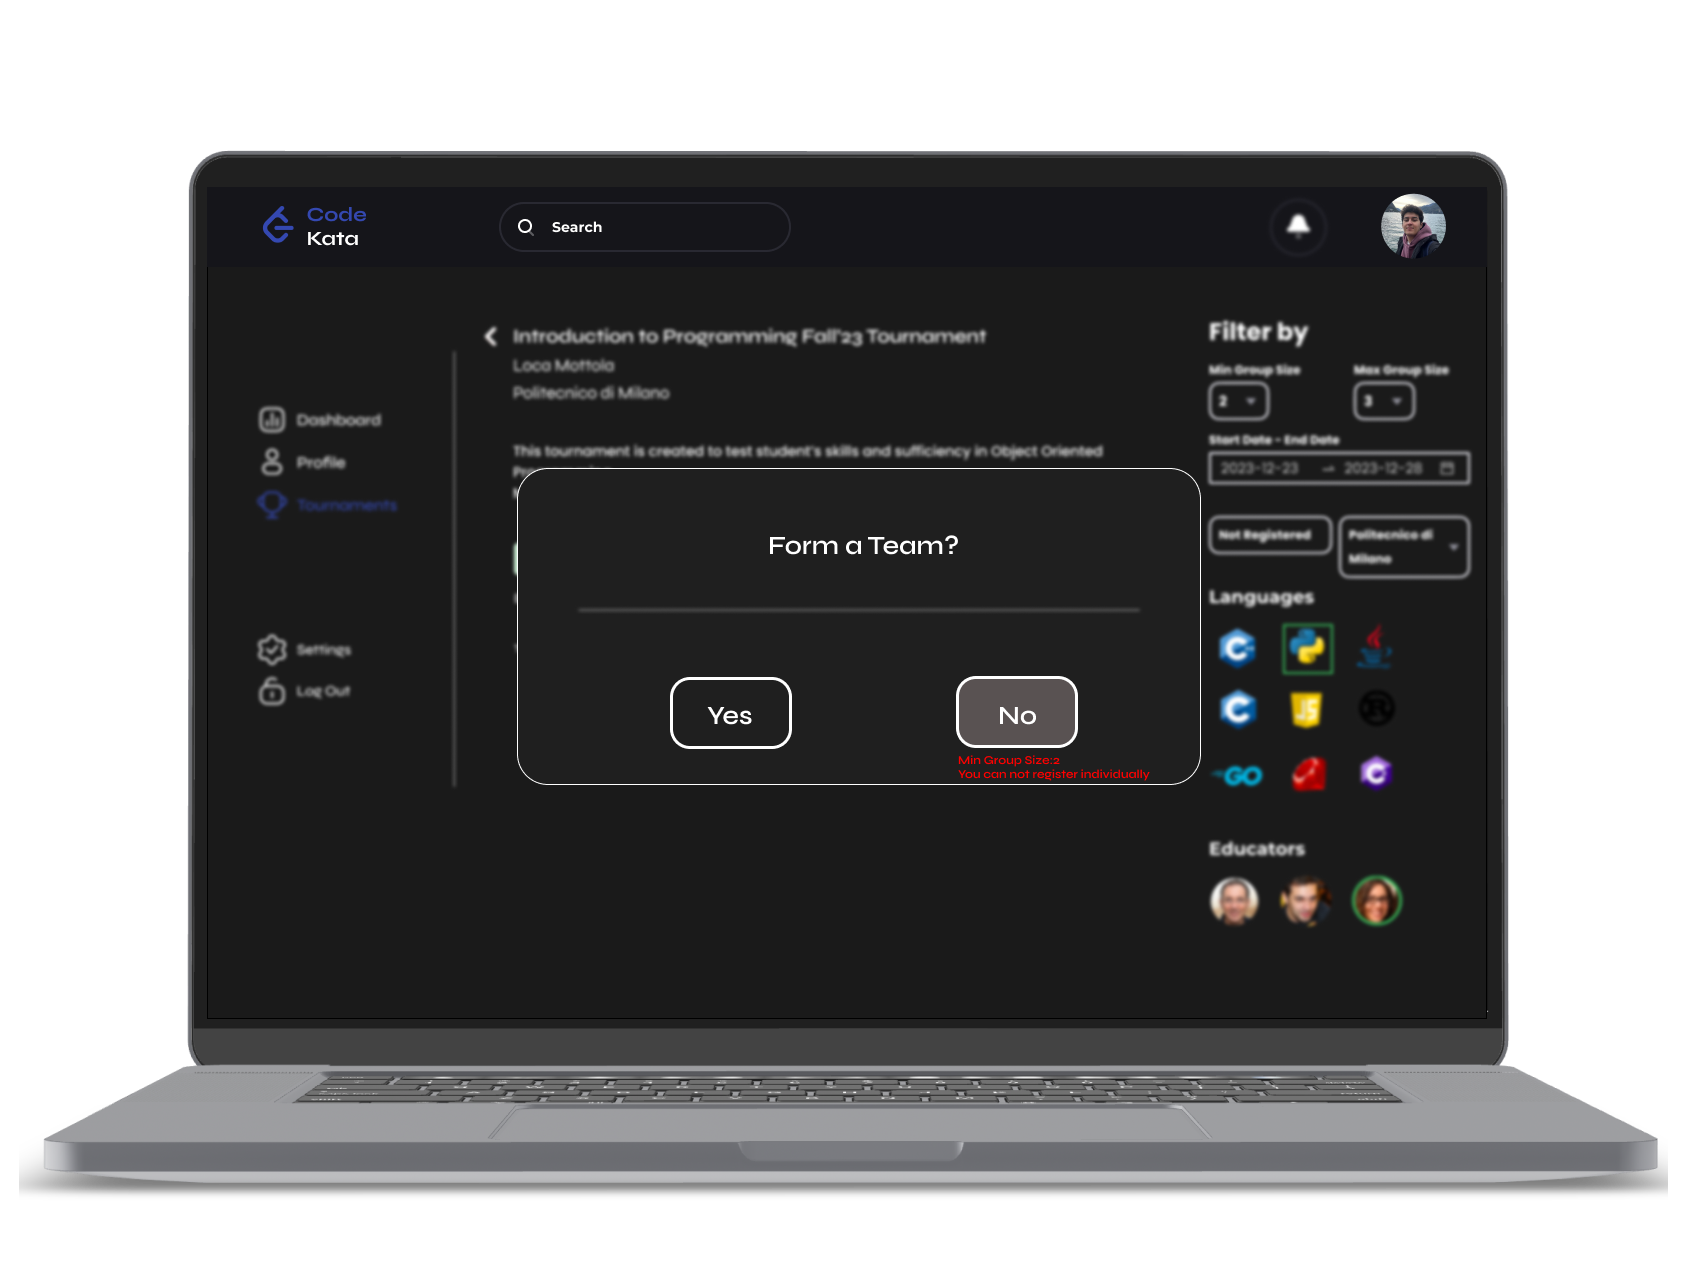
\includegraphics[scale=0.13]{Images/ui-ux/student_battle_register/student_battle_register_2.png}
% 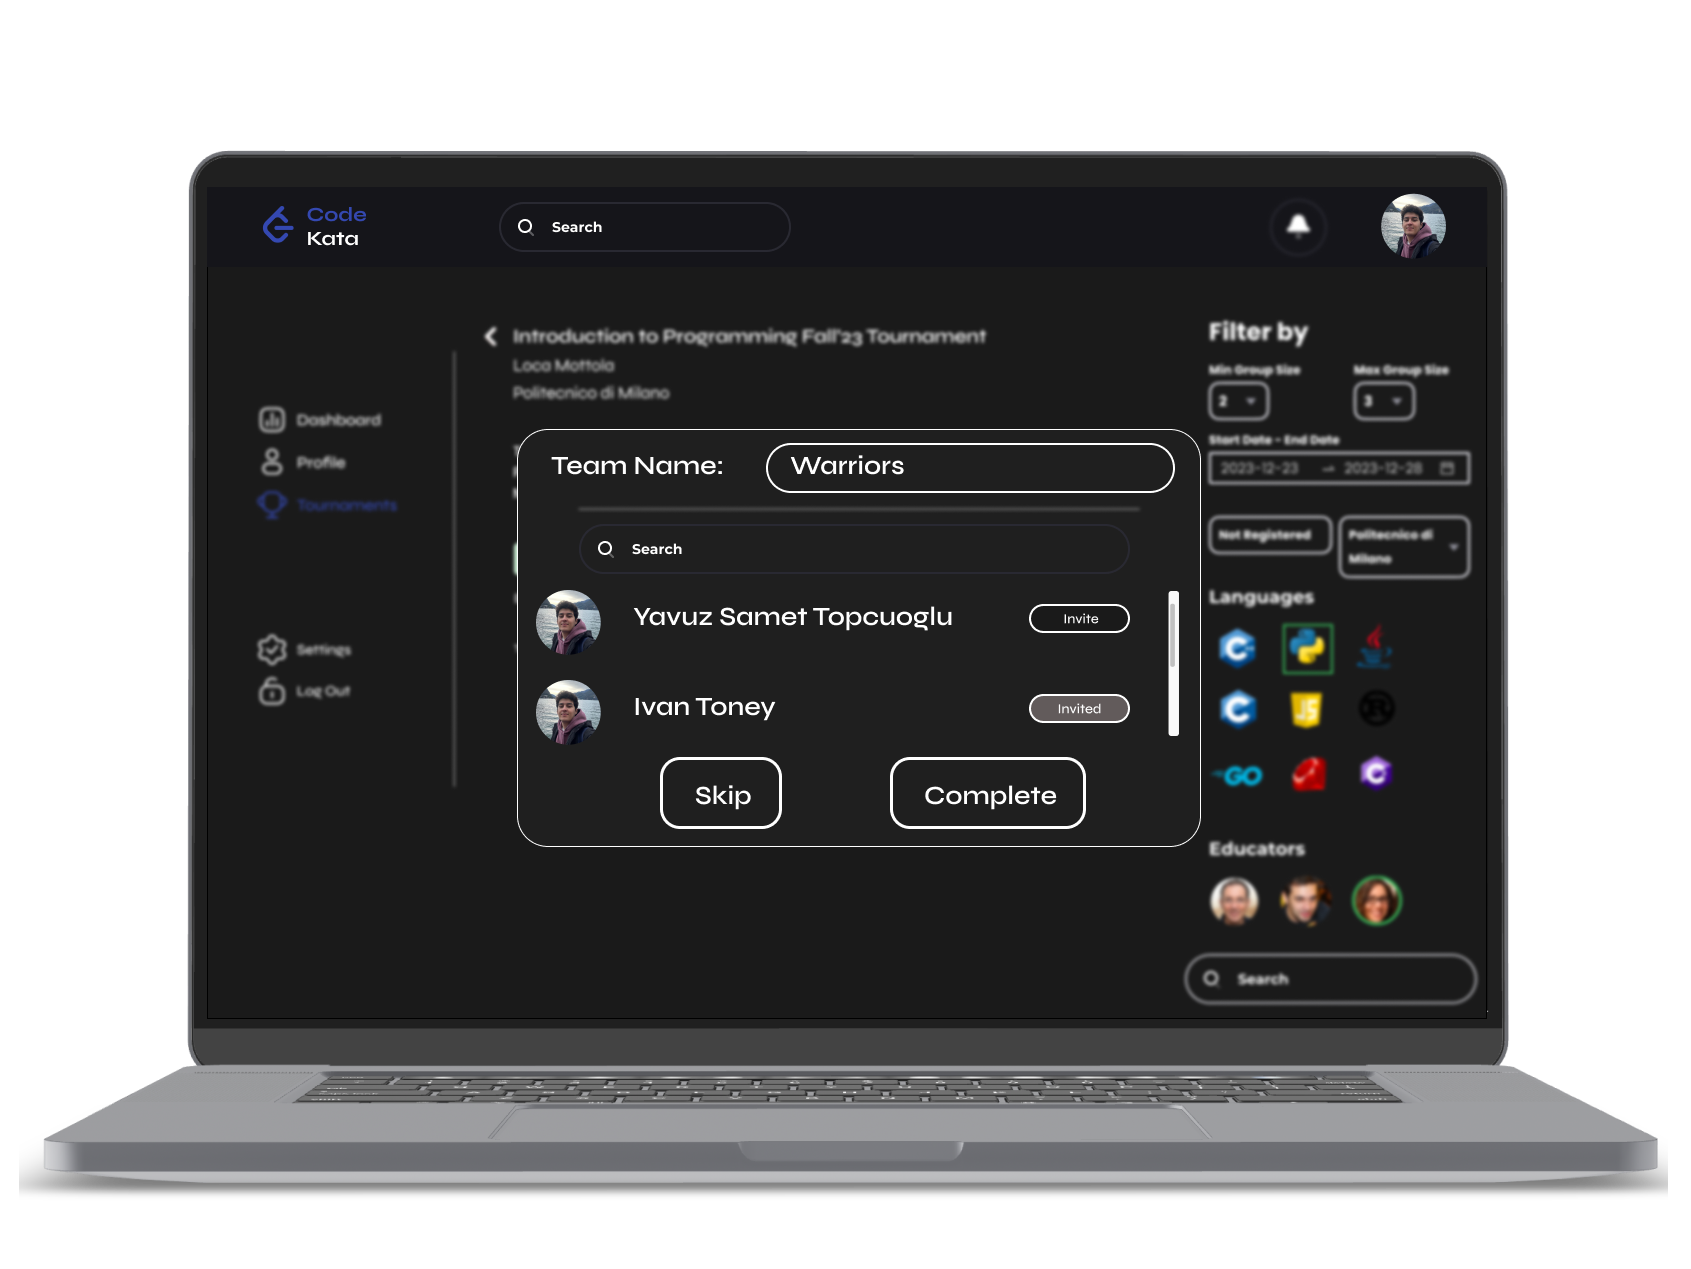
\includegraphics[scale=0.13]{Images/ui-ux/student_battle_register/student_battle_register_3.png}
% \\ (a) Student Registers Battle
% \end{center}
% \newpage
% \begin{center}
% 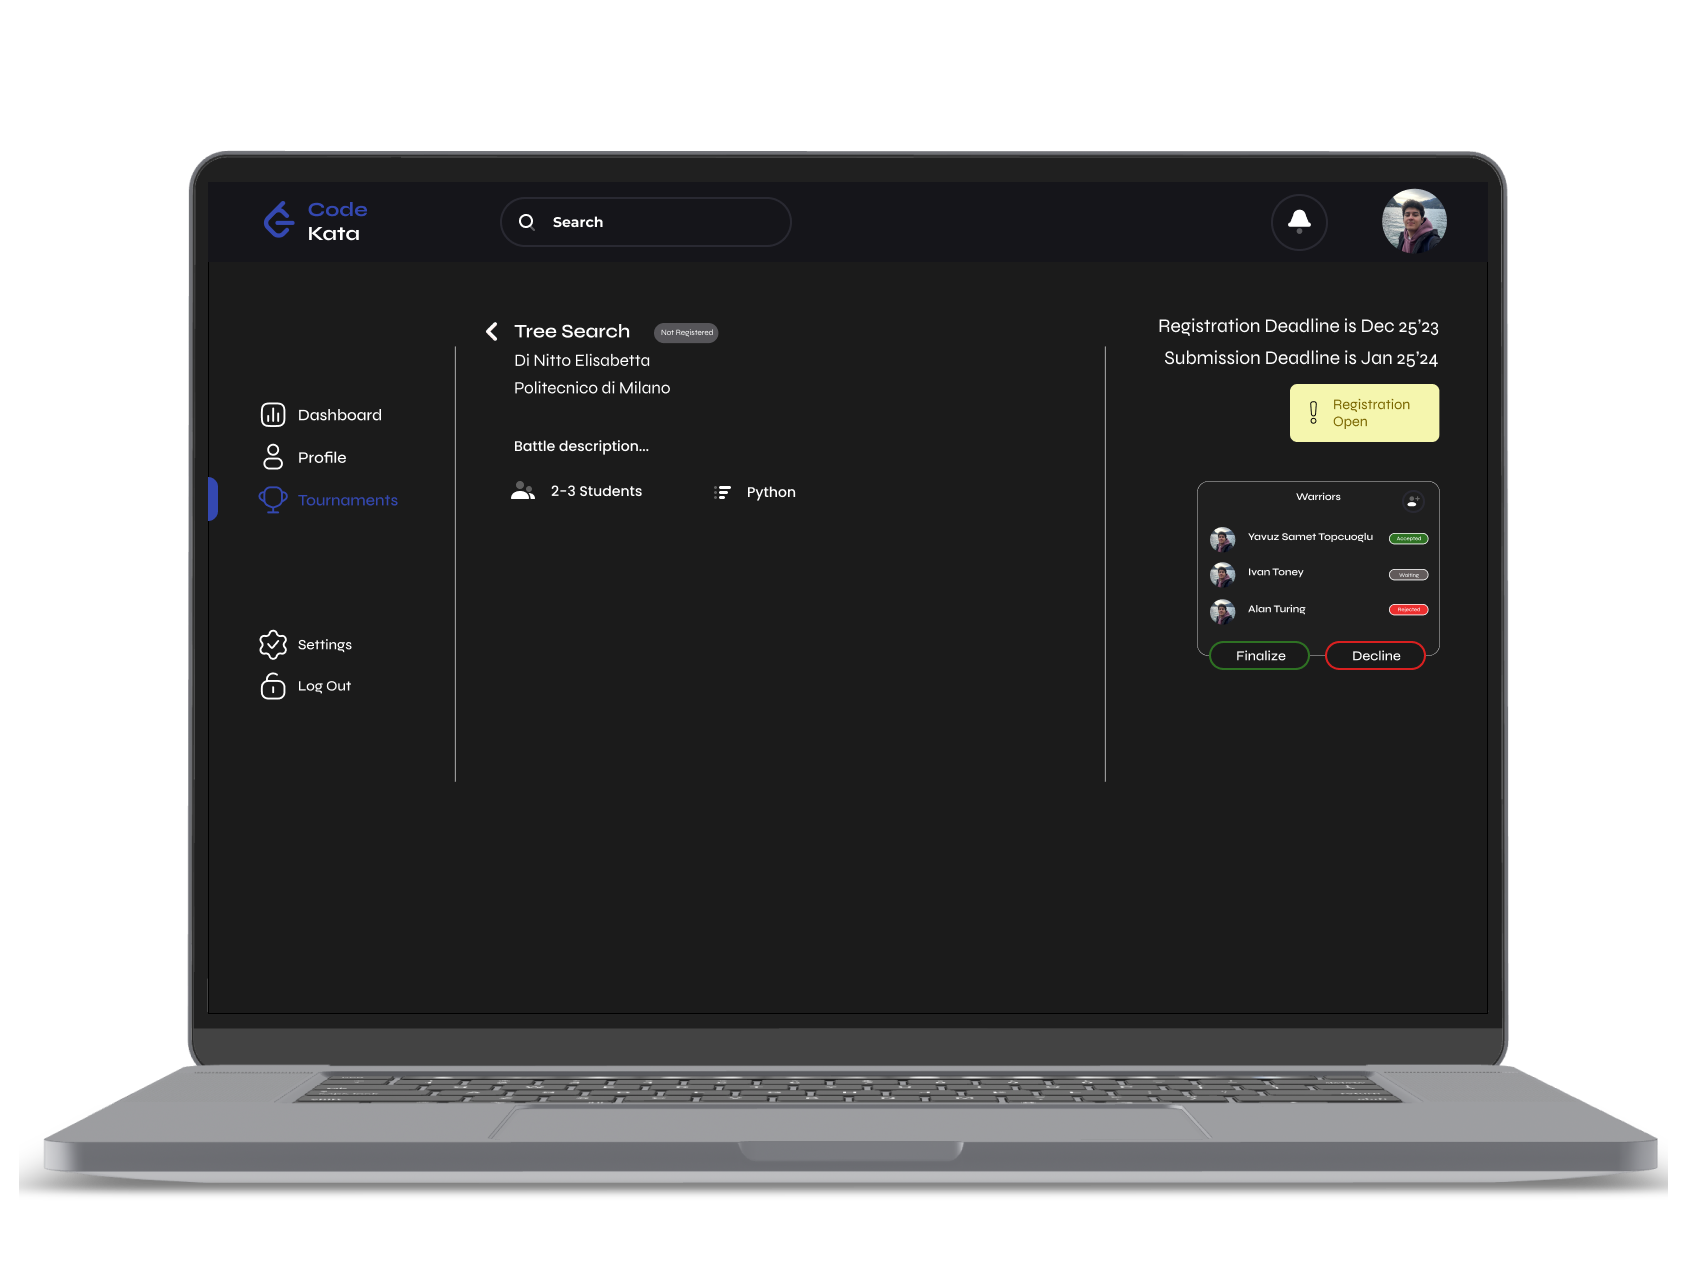
\includegraphics[scale=0.13]{Images/ui-ux/student_battle/student_battle_1.png}
% 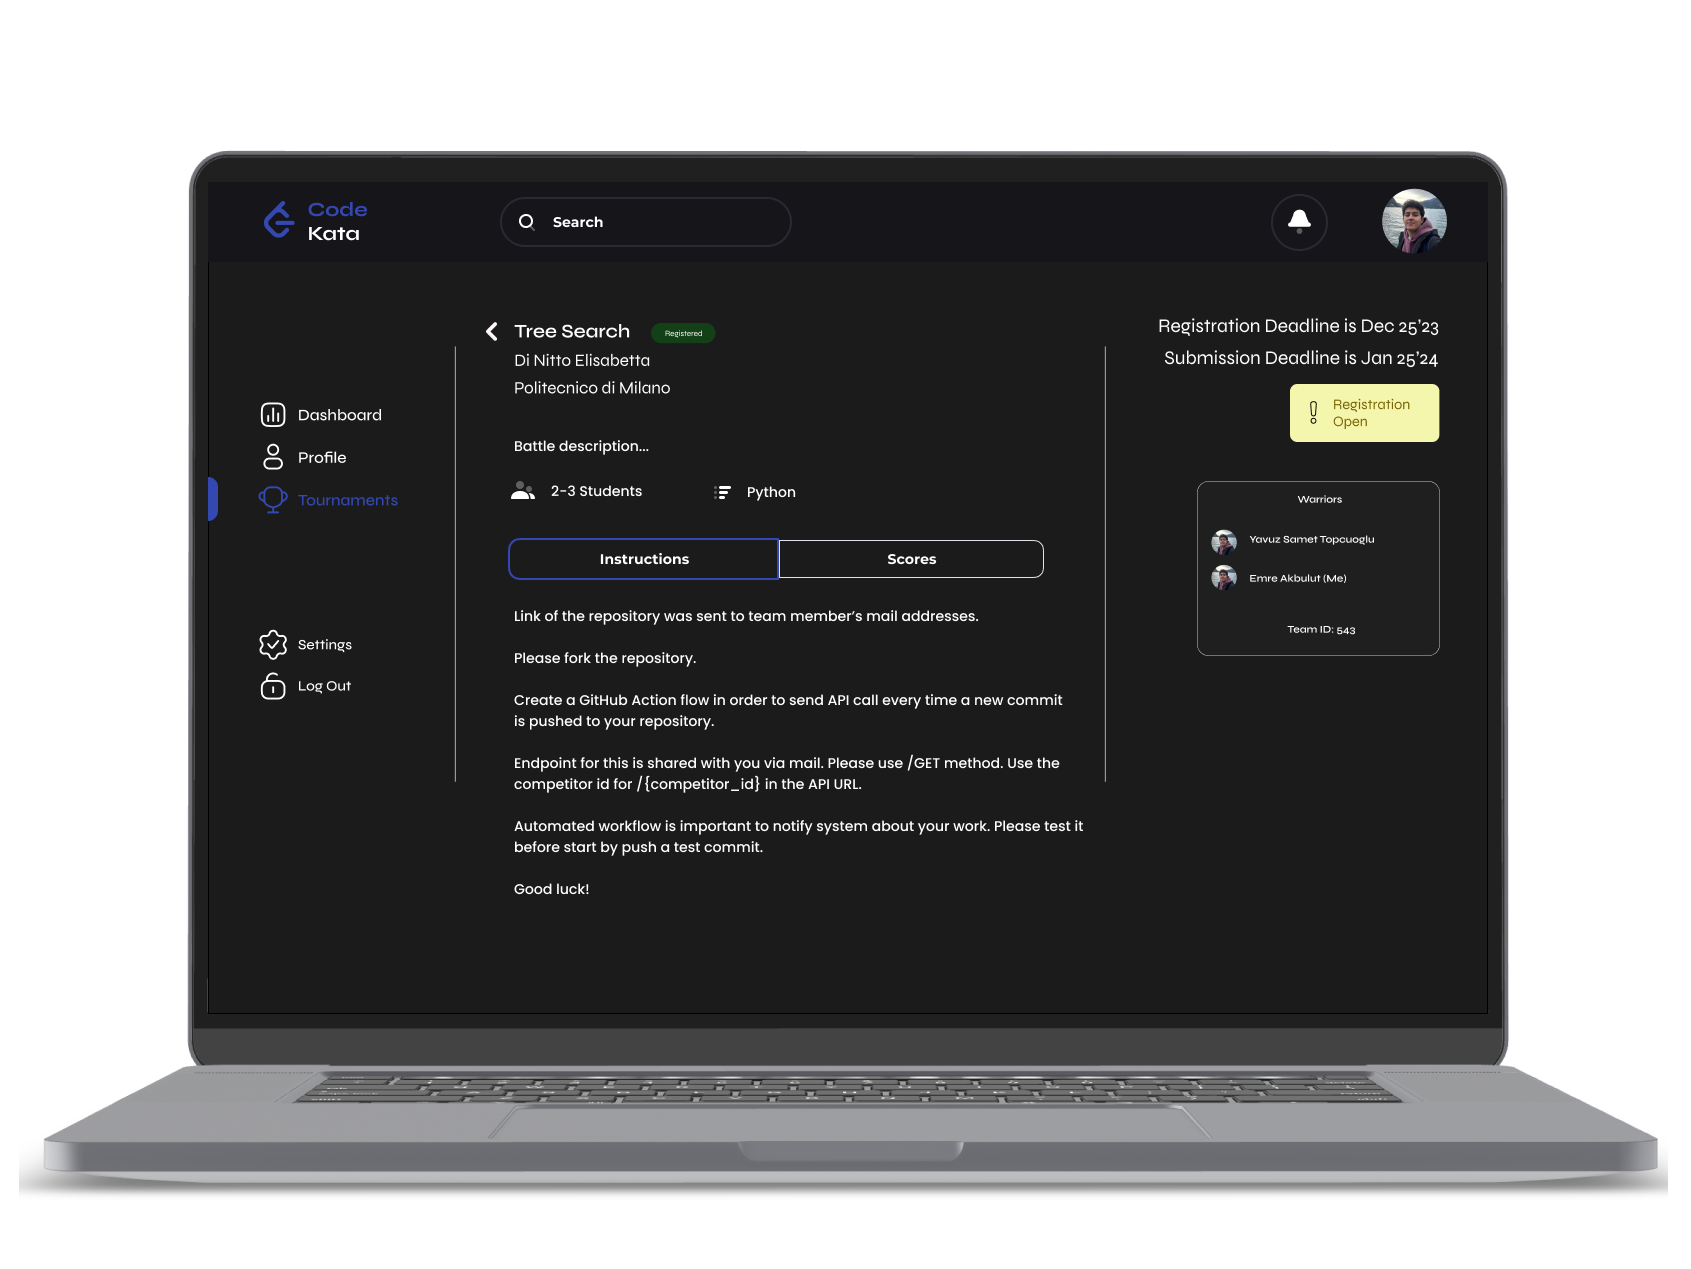
\includegraphics[scale=0.13]{Images/ui-ux/student_battle/student_battle_2.png}
% 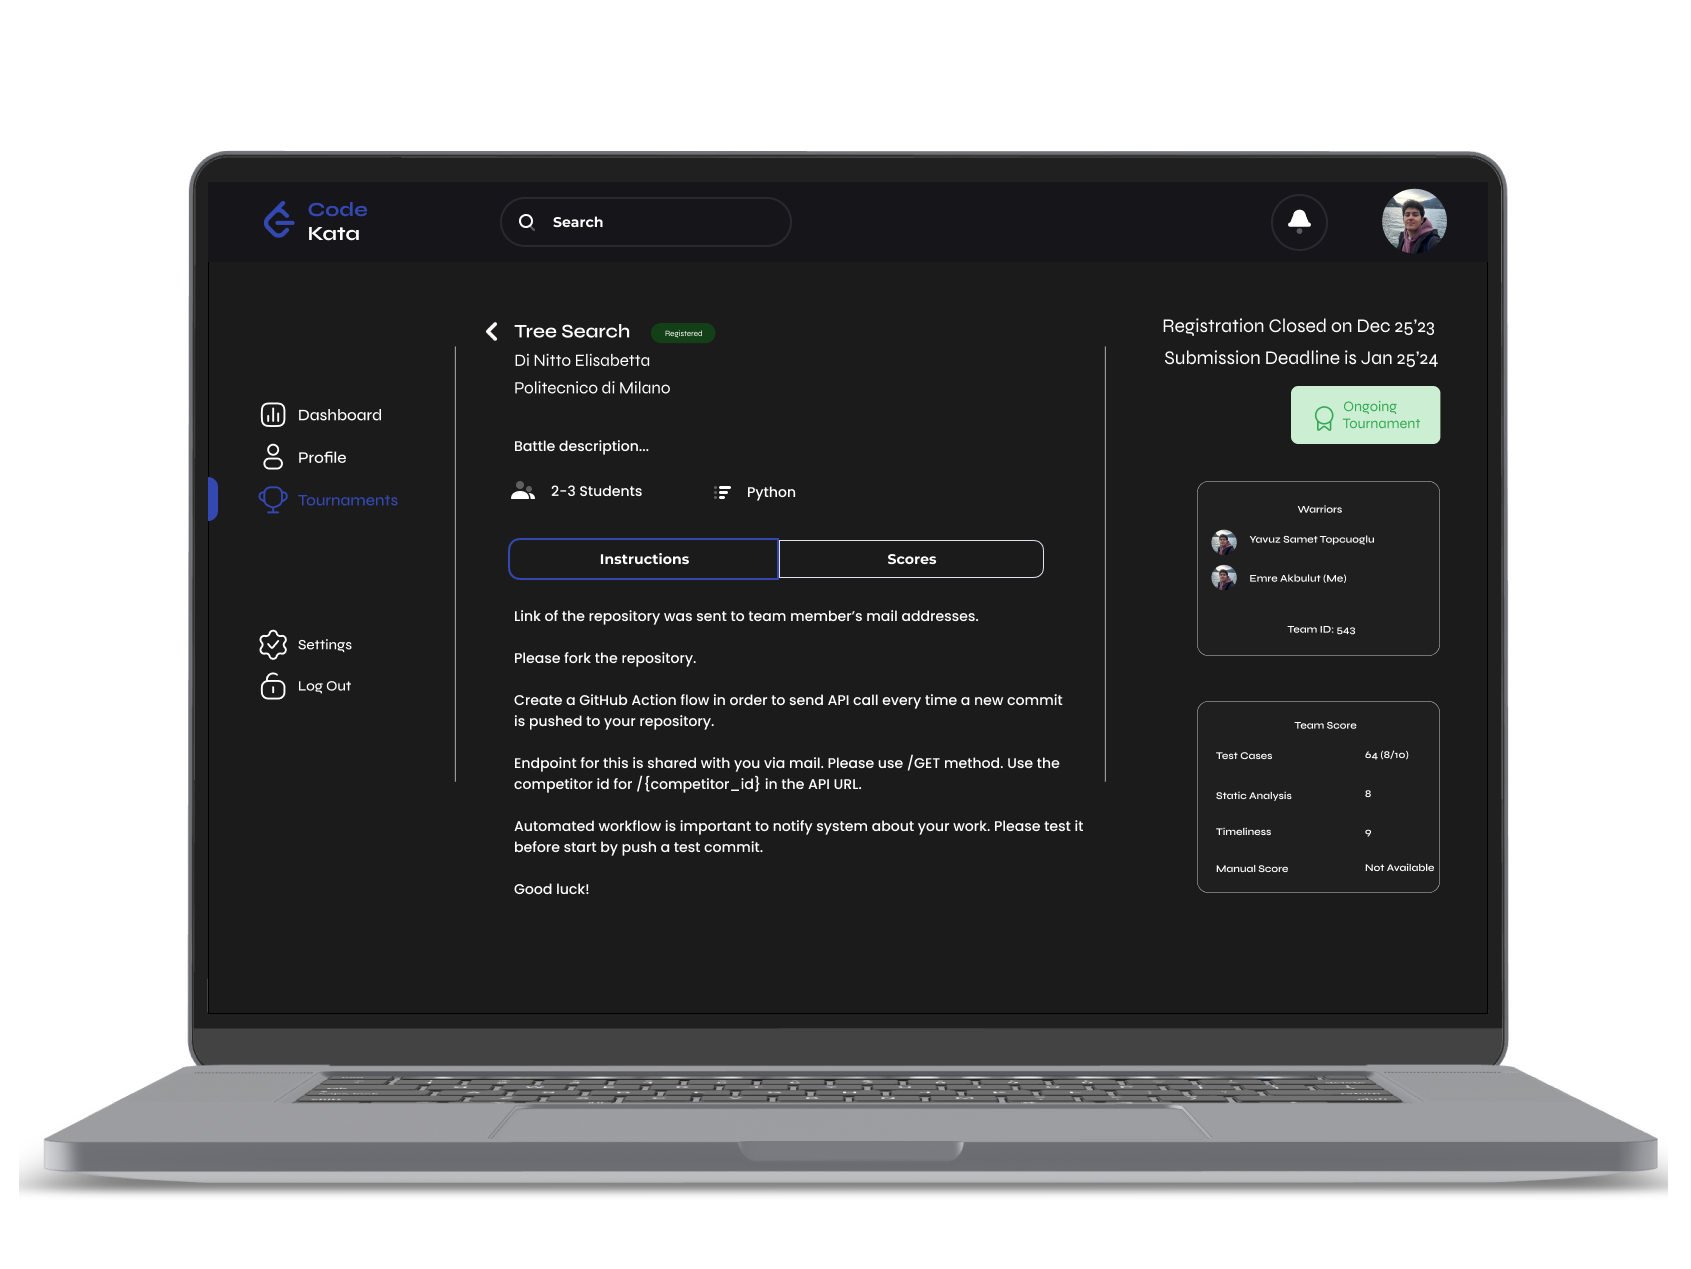
\includegraphics[scale=0.13]{Images/ui-ux/student_battle/student_battle_3.png}
% 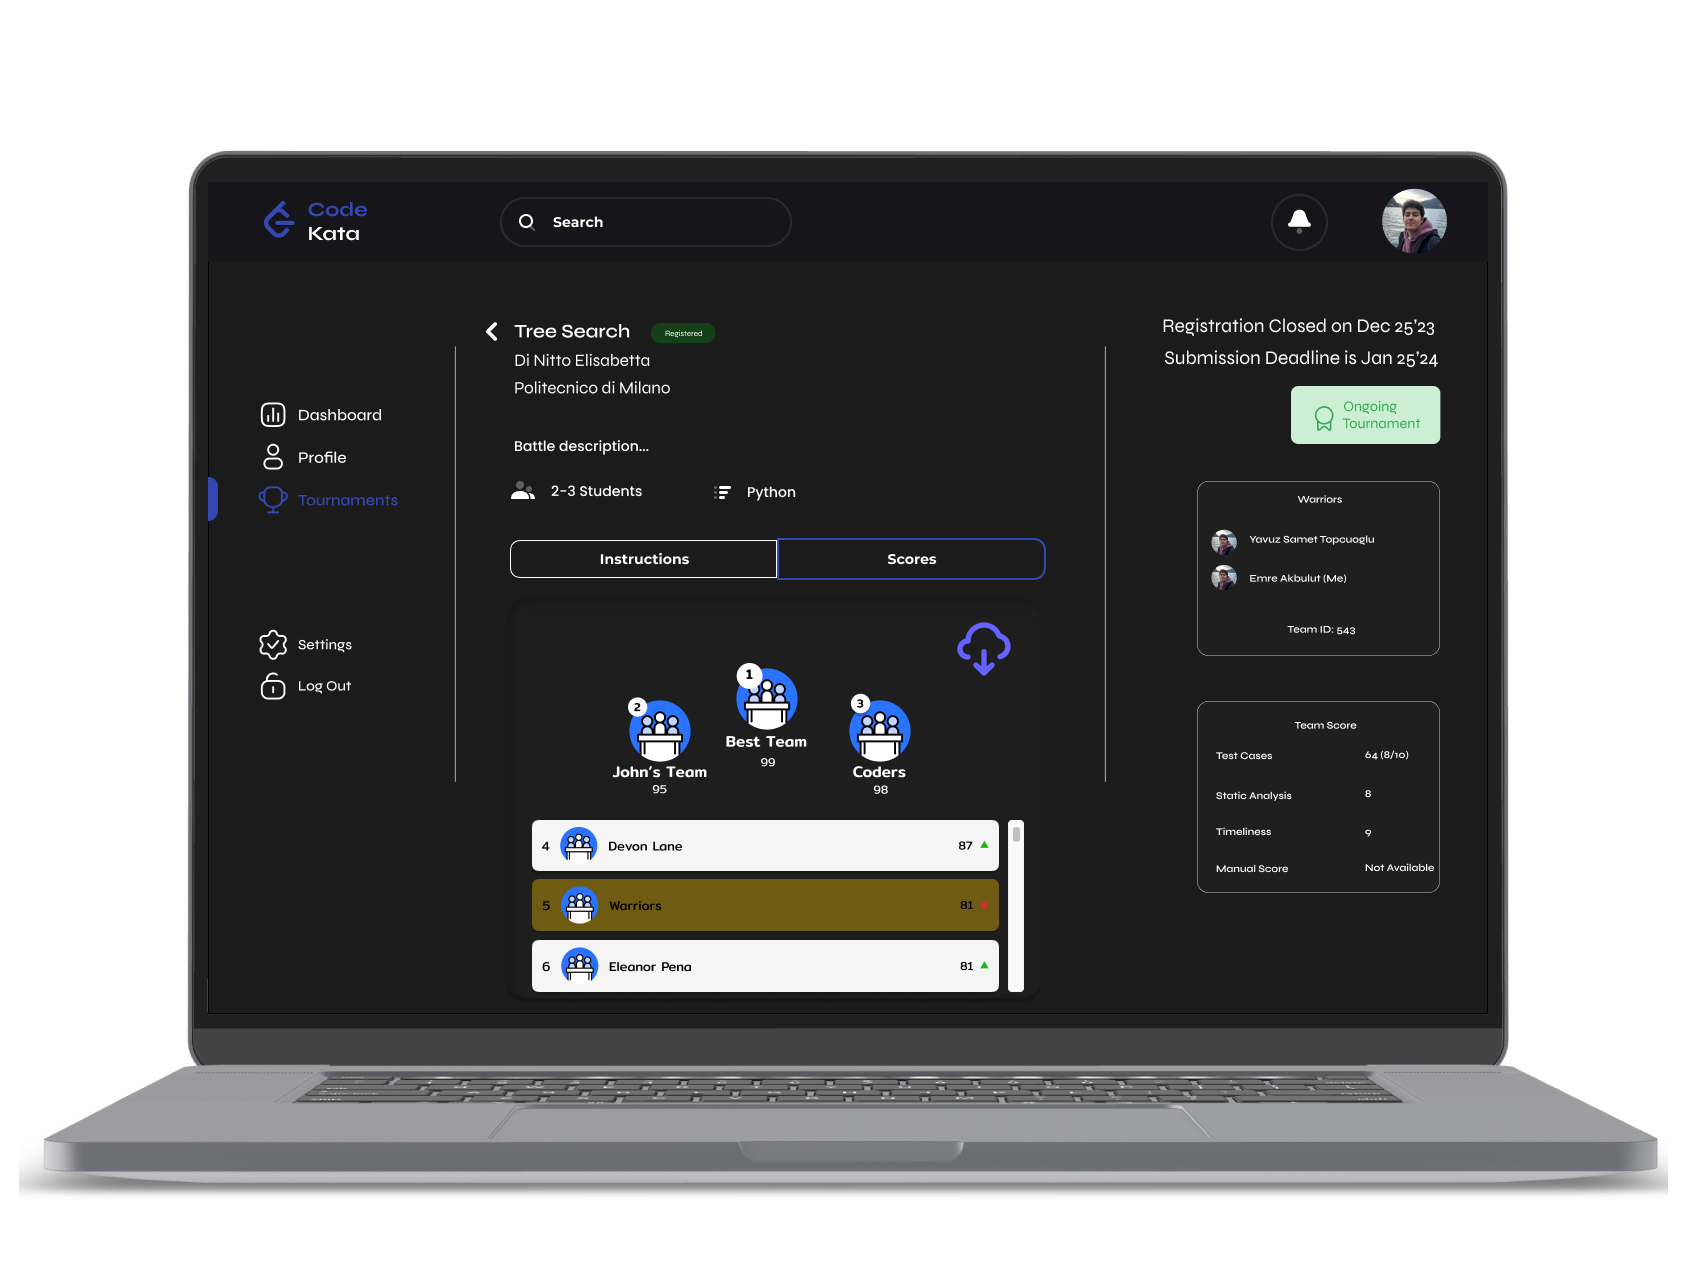
\includegraphics[scale=0.13]{Images/ui-ux/student_battle/student_battle_4.png}
%       (a) Battle Screen for Student
% \end{center}

% \begin{center}
% 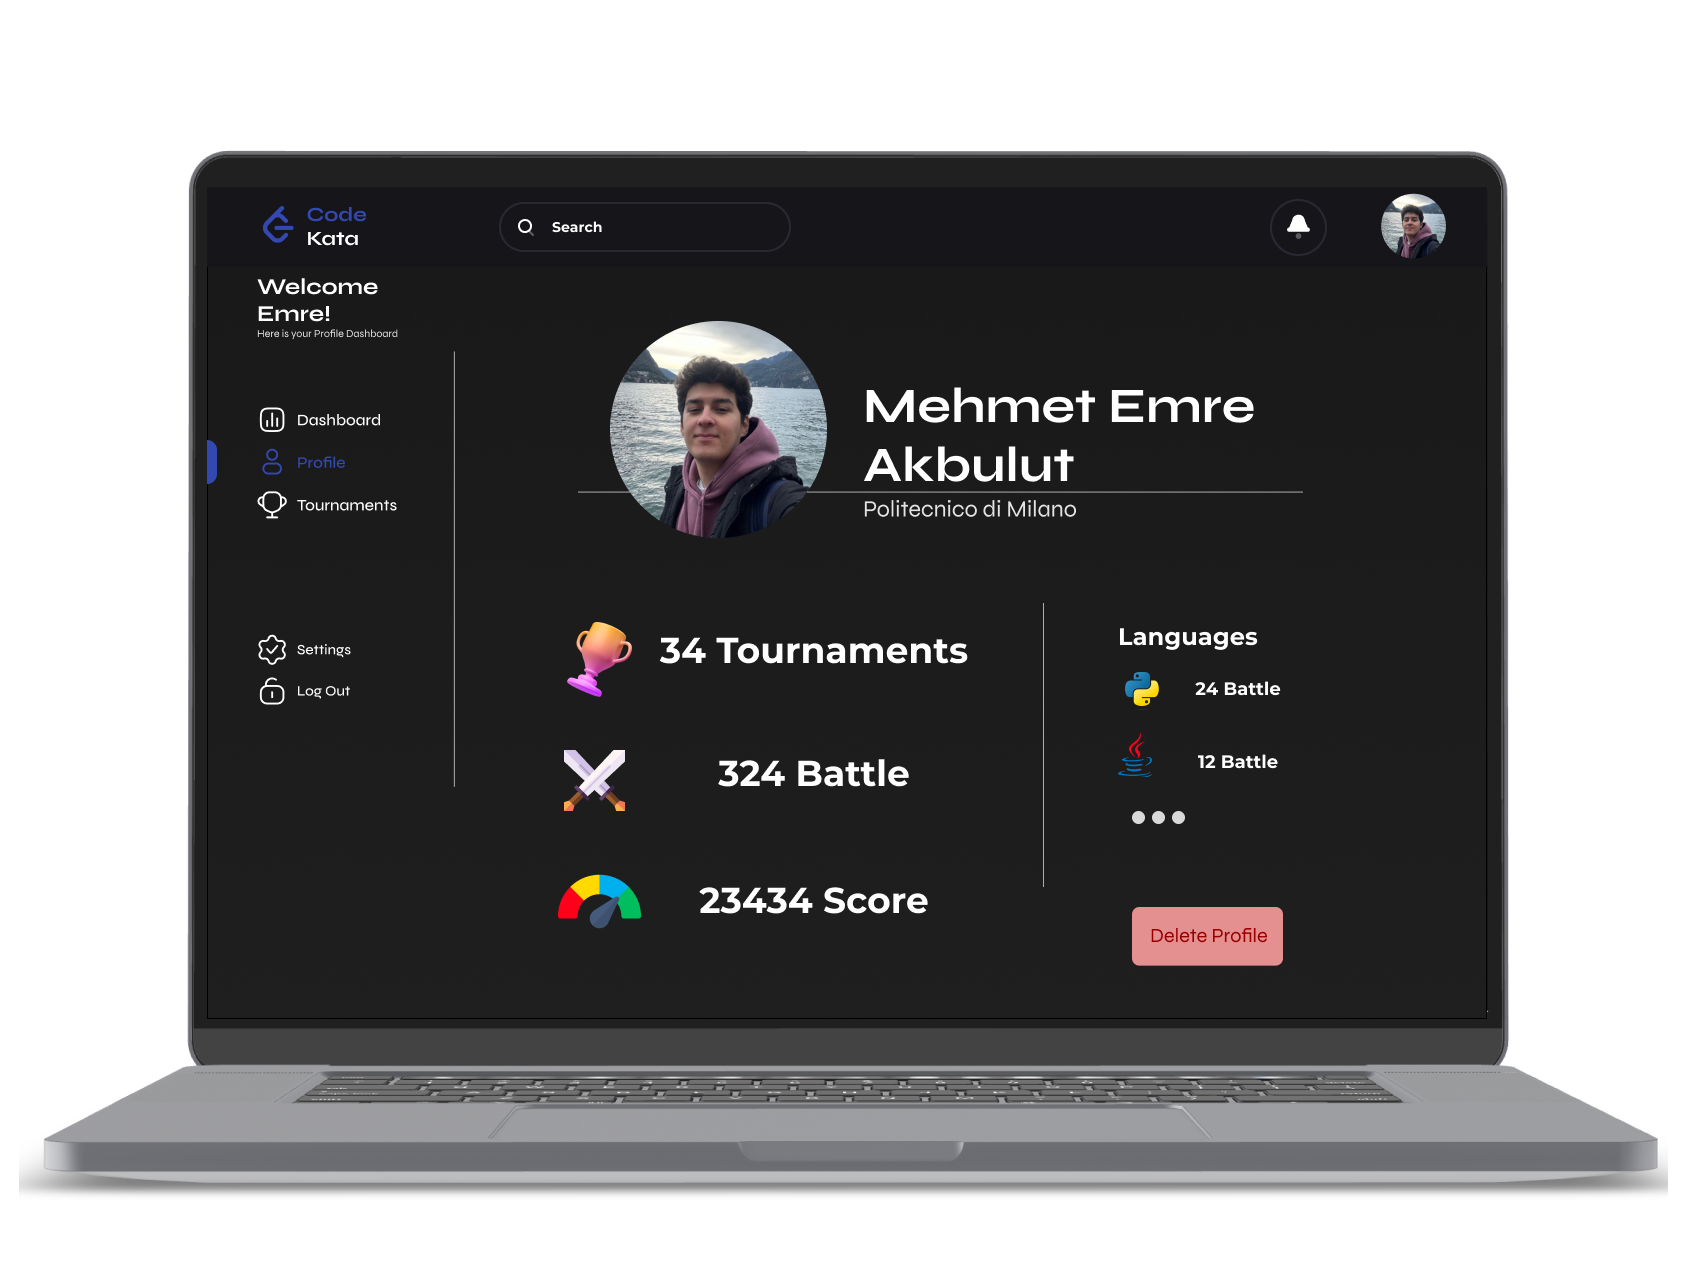
\includegraphics[scale=0.13]{Images/ui-ux/student_profile_settings/student_profile.png}
% 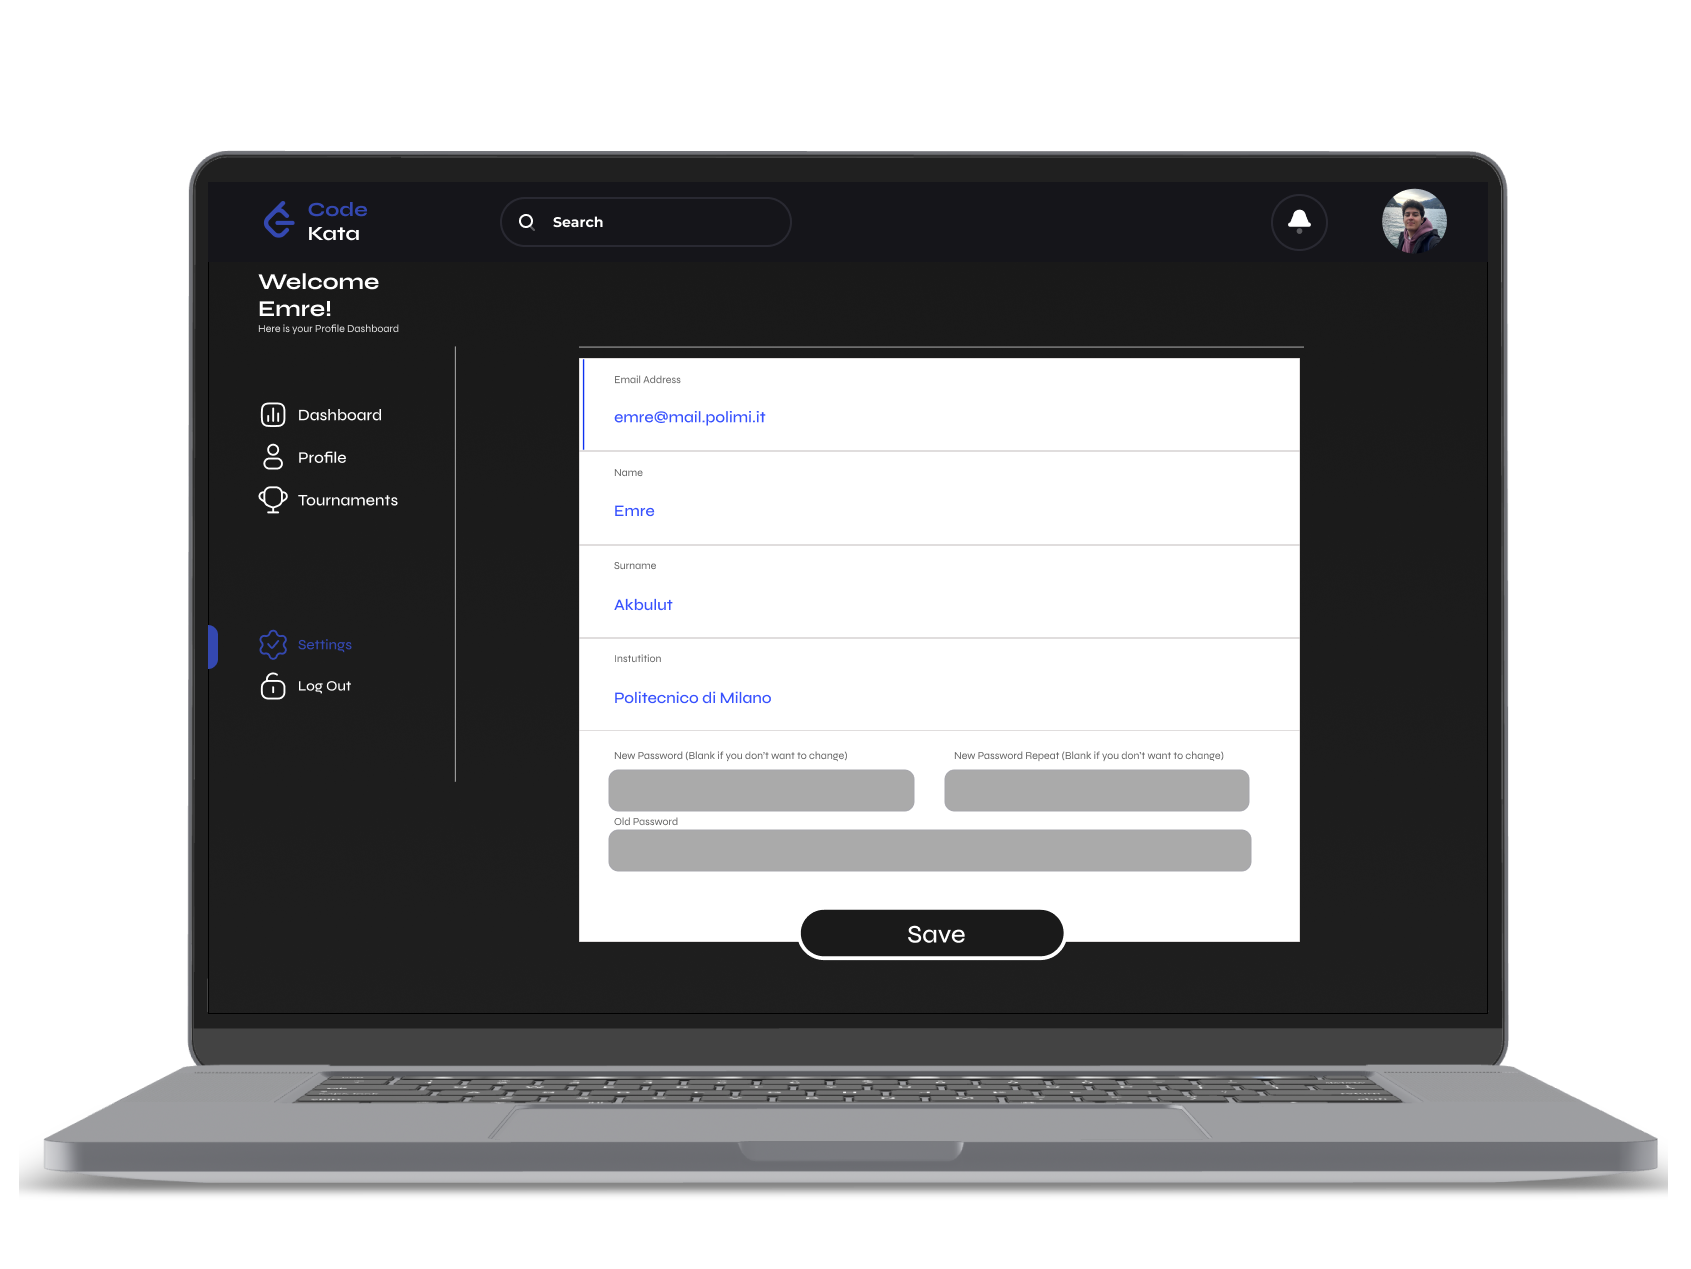
\includegraphics[scale=0.13]{Images/ui-ux/student_profile_settings/student_settings.png}
%         (a) Profile and Settings for Student
% \end{center}
% \newpage
% \begin{center}
% 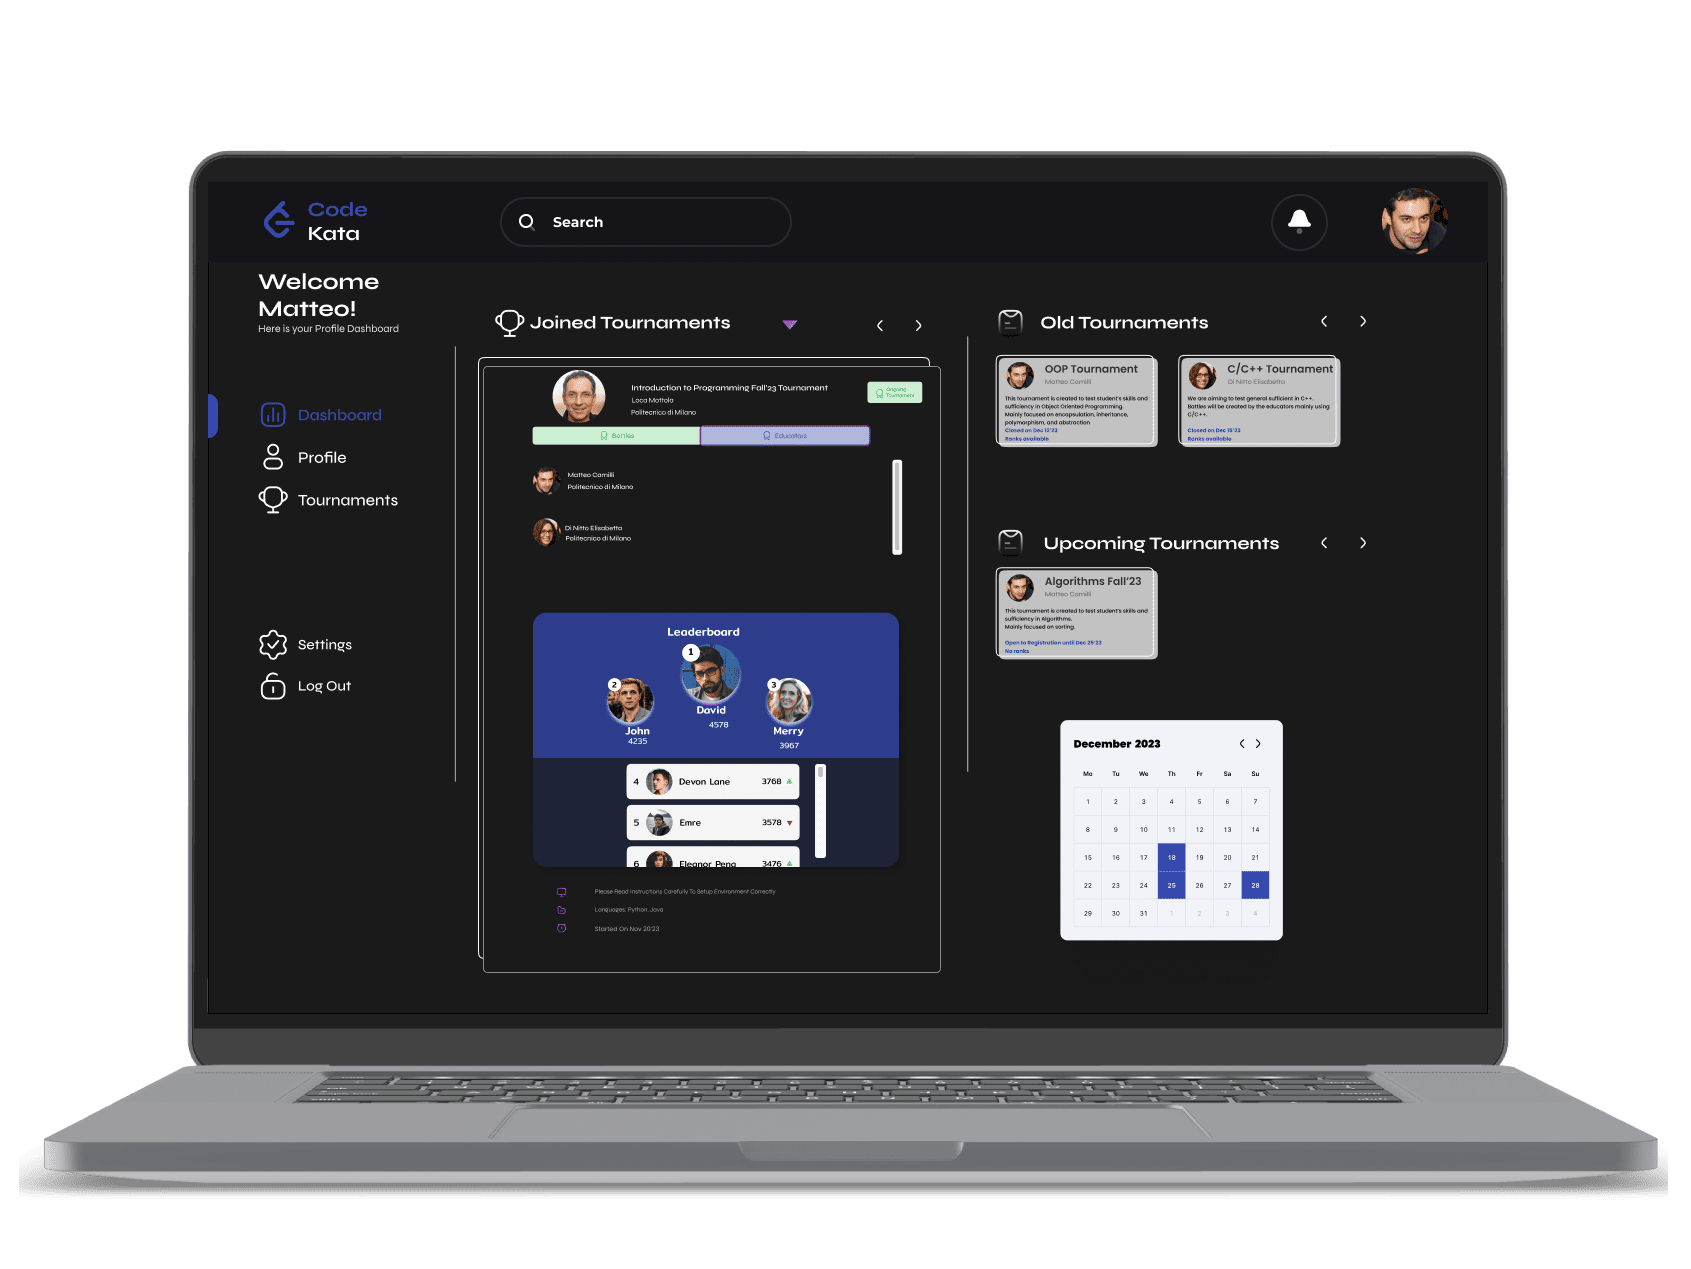
\includegraphics[scale=0.13]{Images/ui-ux/educator_dashboard/educator_dashboard_1.png}
% 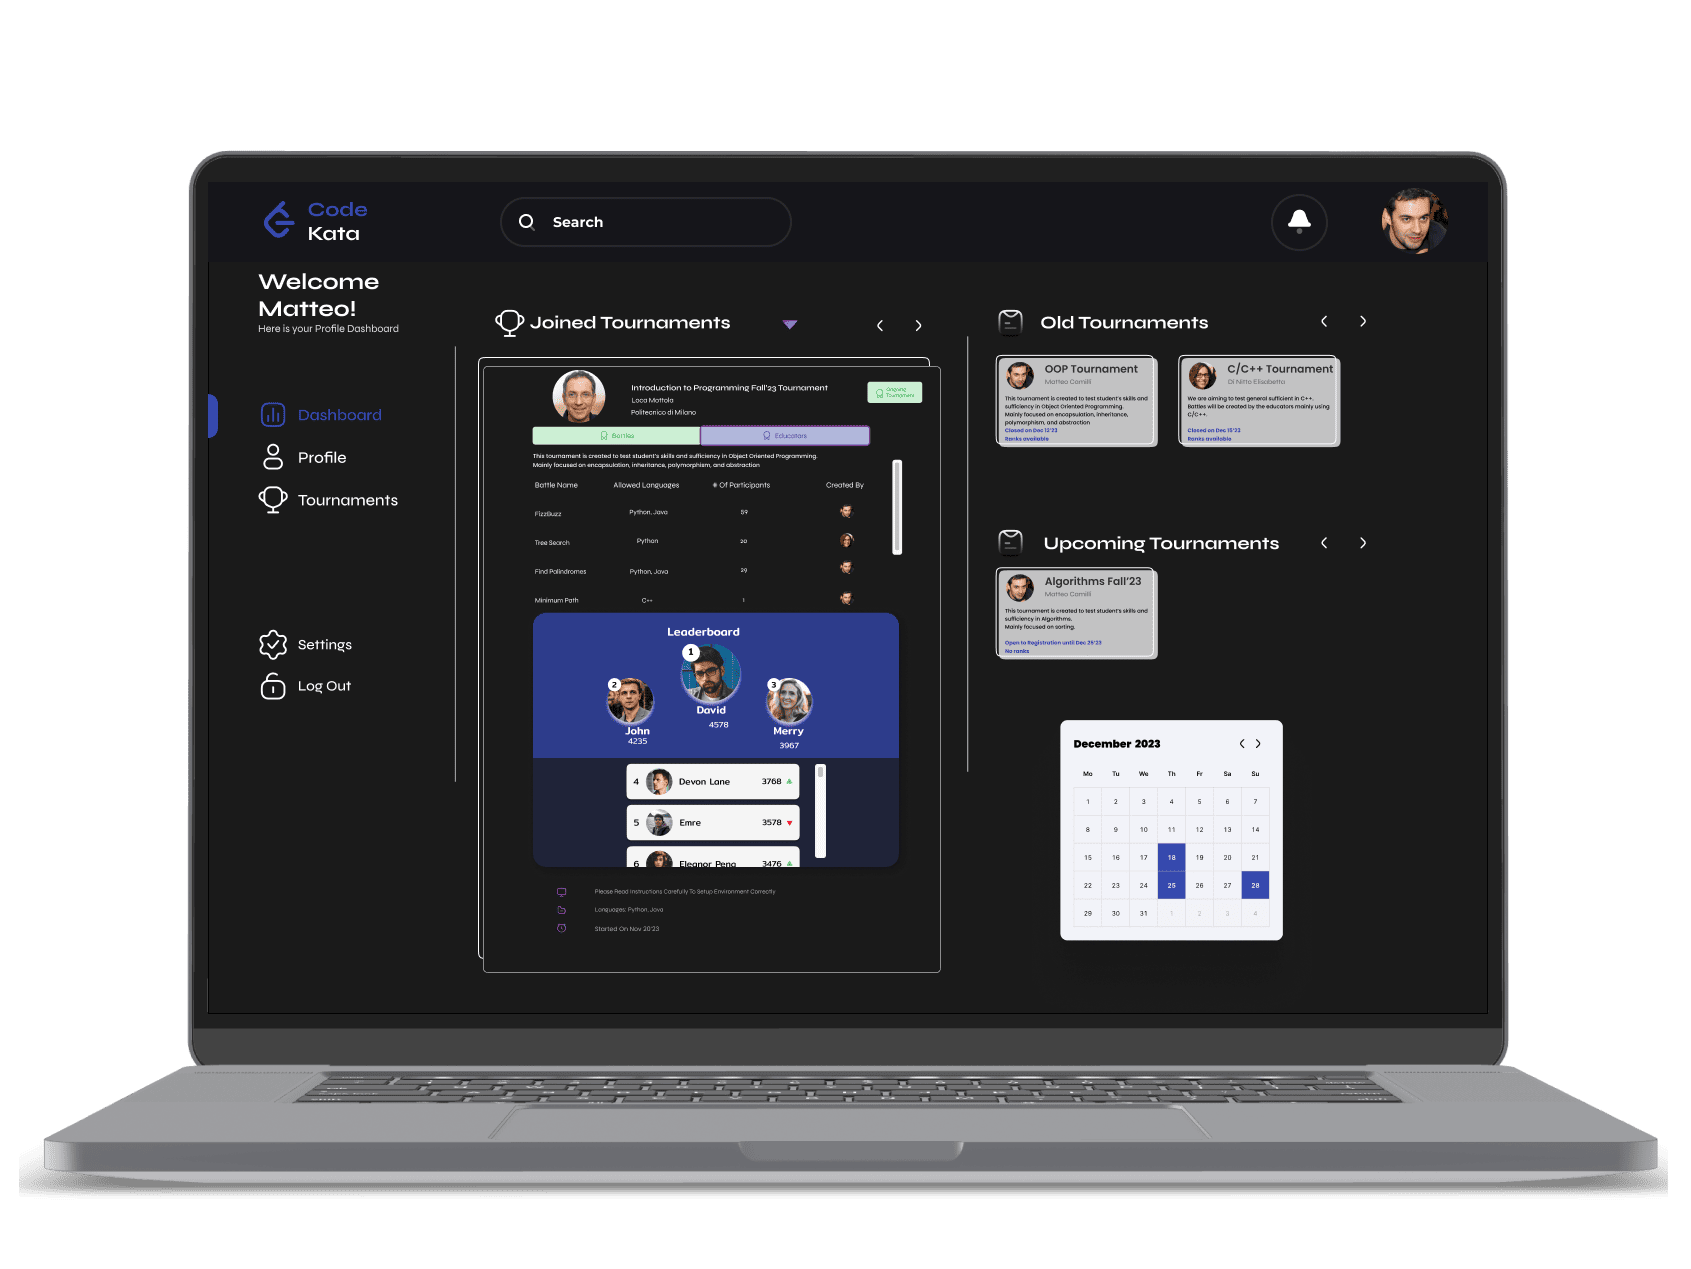
\includegraphics[scale=0.13]{Images/ui-ux/educator_dashboard/educator_dashboard_2.png}
% 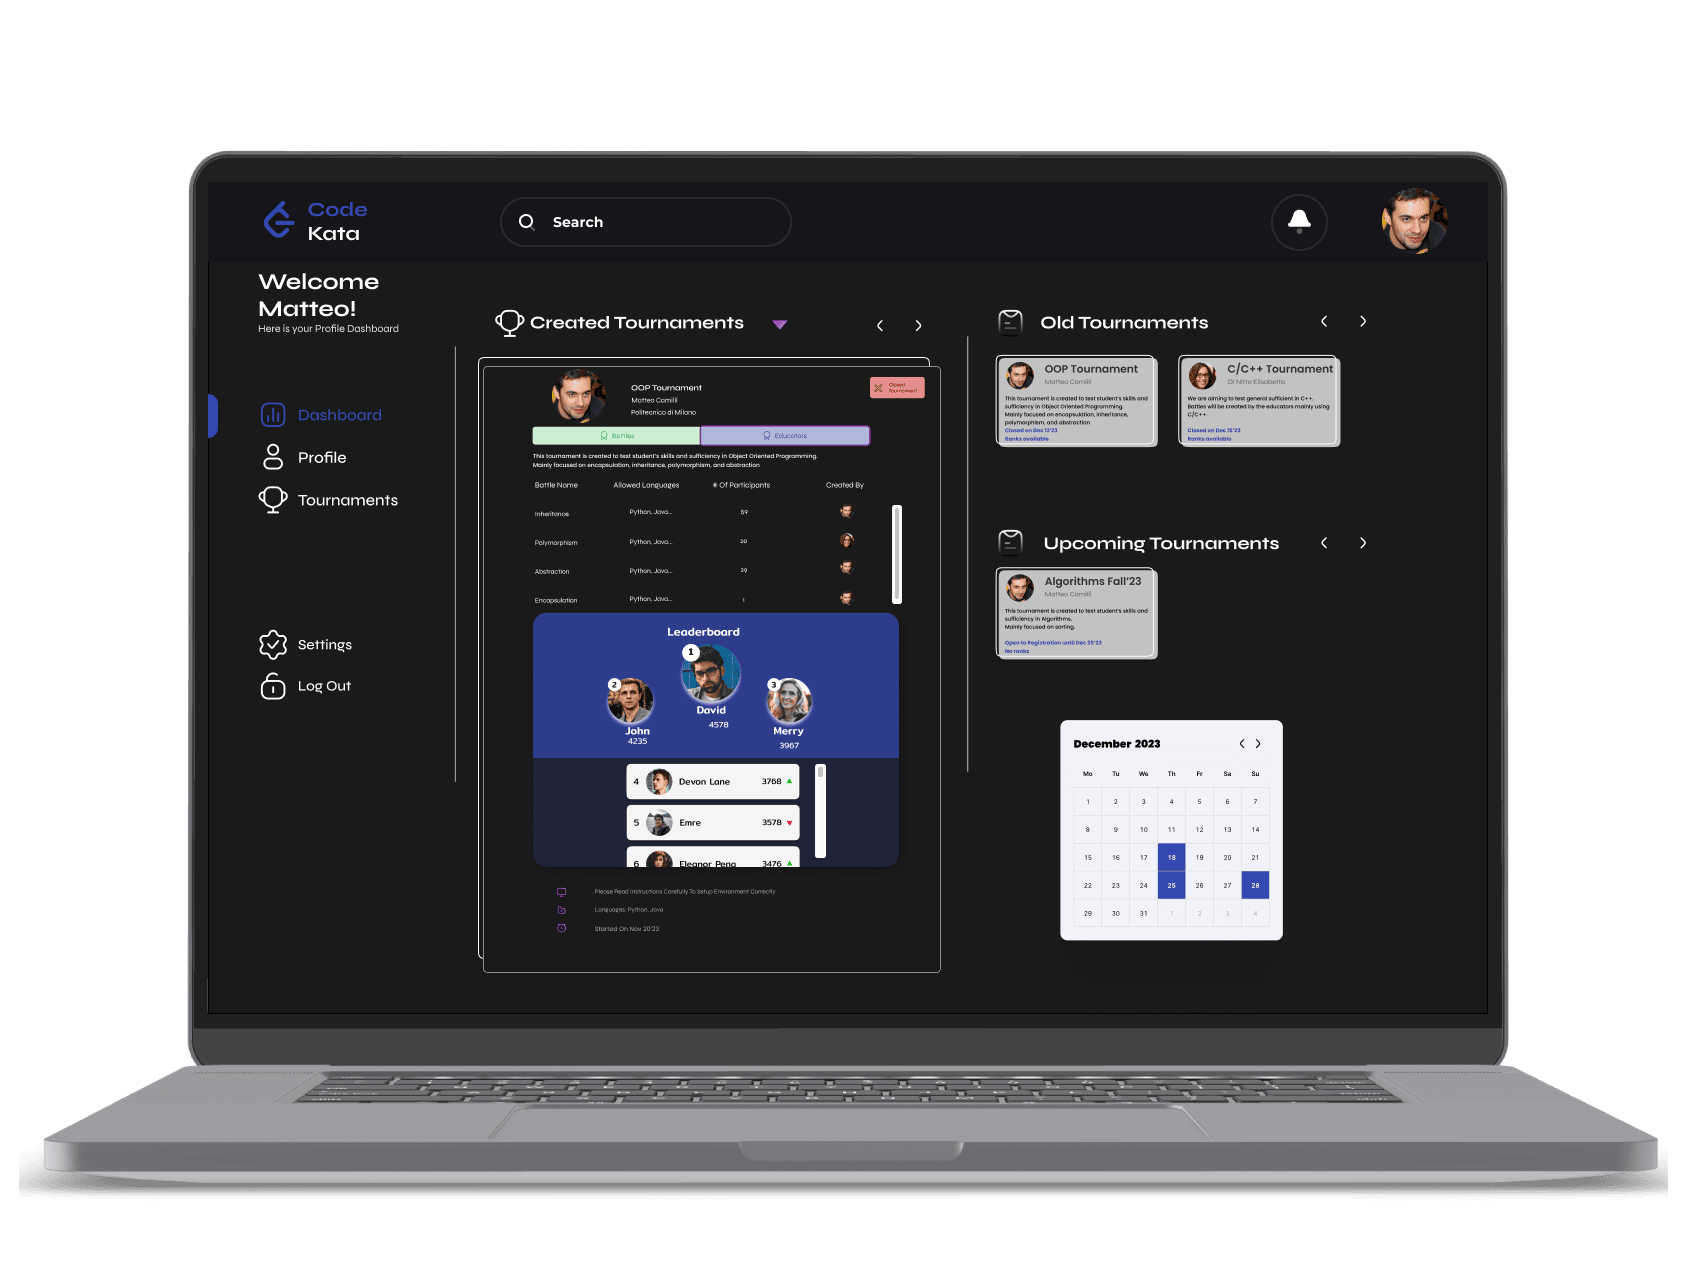
\includegraphics[scale=0.13]{Images/ui-ux/educator_dashboard/educator_dashboard_3.png}
% \\ (a) Educator Dashboard
% \end{center}
% \begin{center}
% 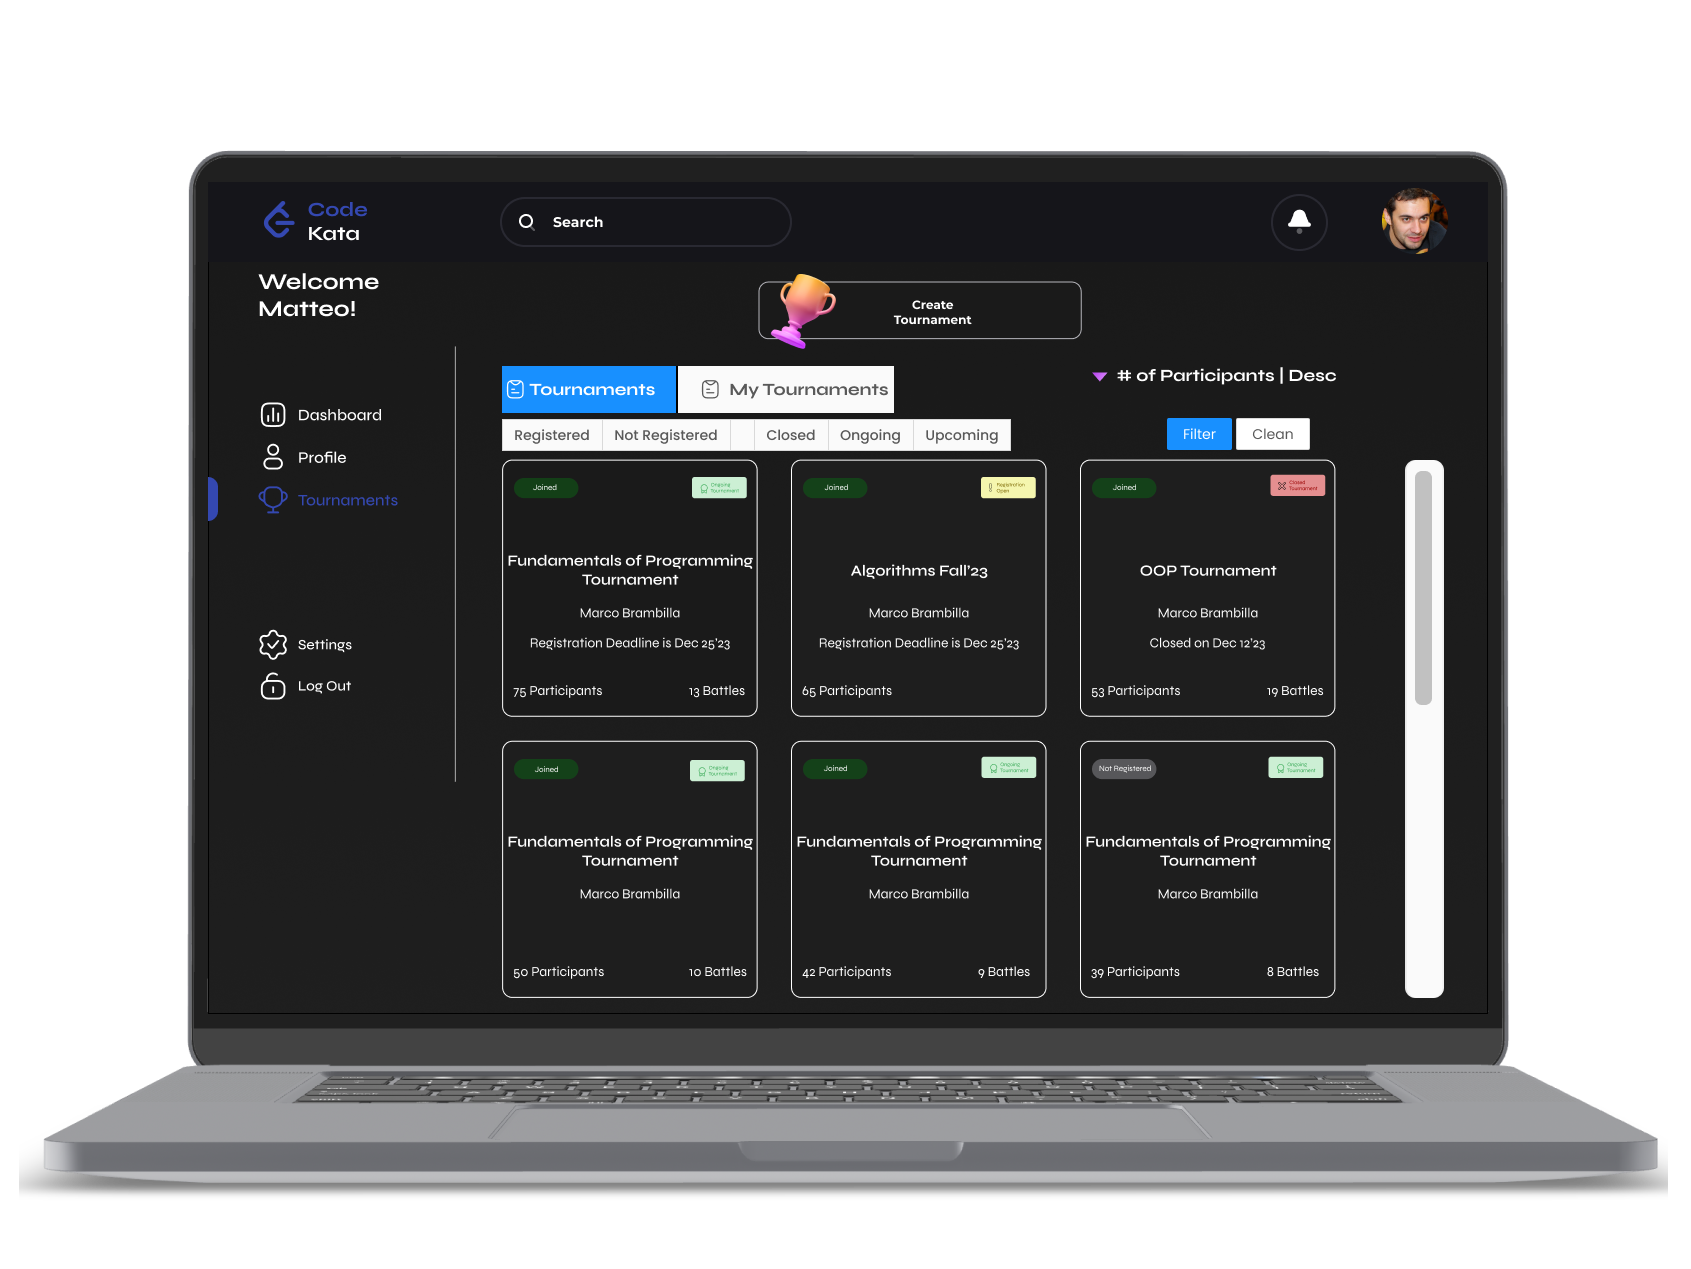
\includegraphics[scale=0.13]{Images/ui-ux/educator_tournaments/educator_tournaments_1.png}
% 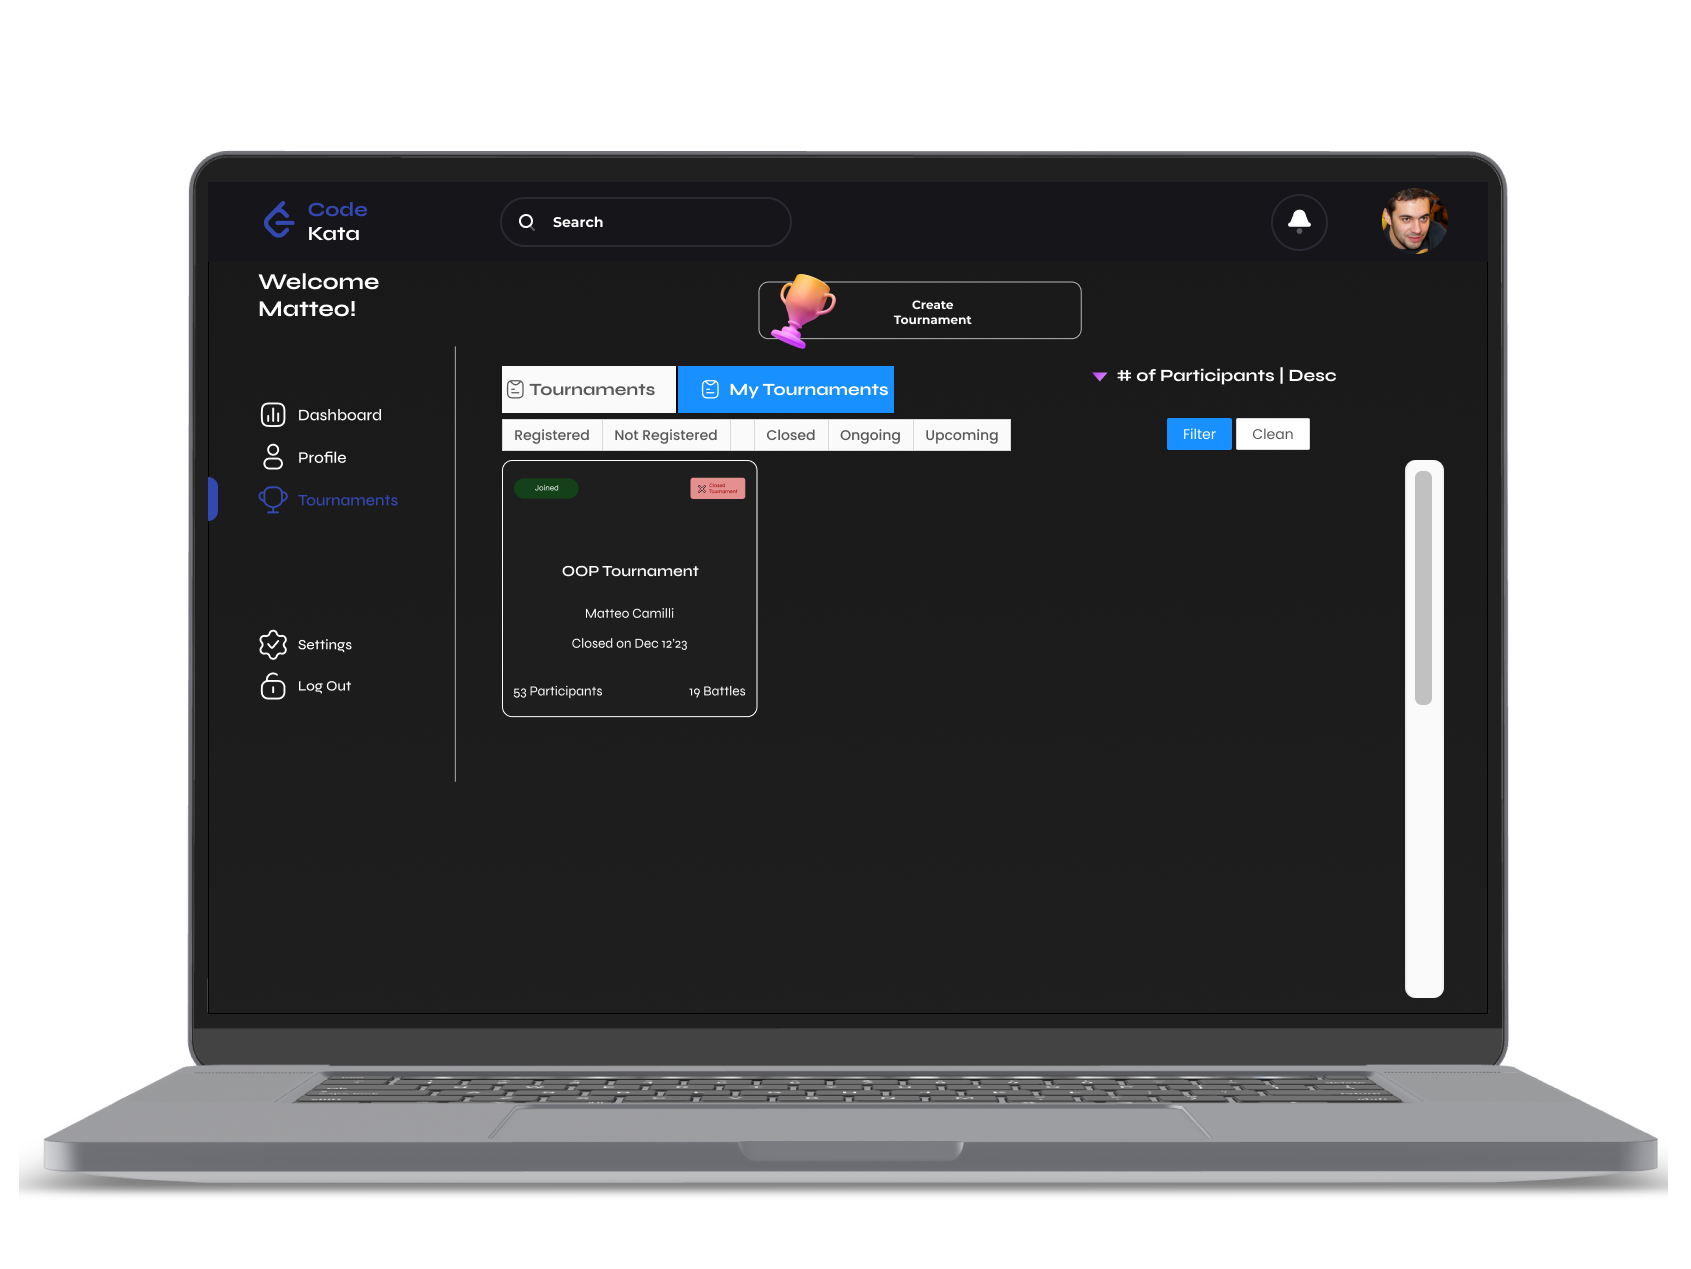
\includegraphics[scale=0.13]{Images/ui-ux/educator_tournaments/educator_tournaments_2.png}
%         (a) Educator Tournaments
% \end{center}
% \begin{center}
% 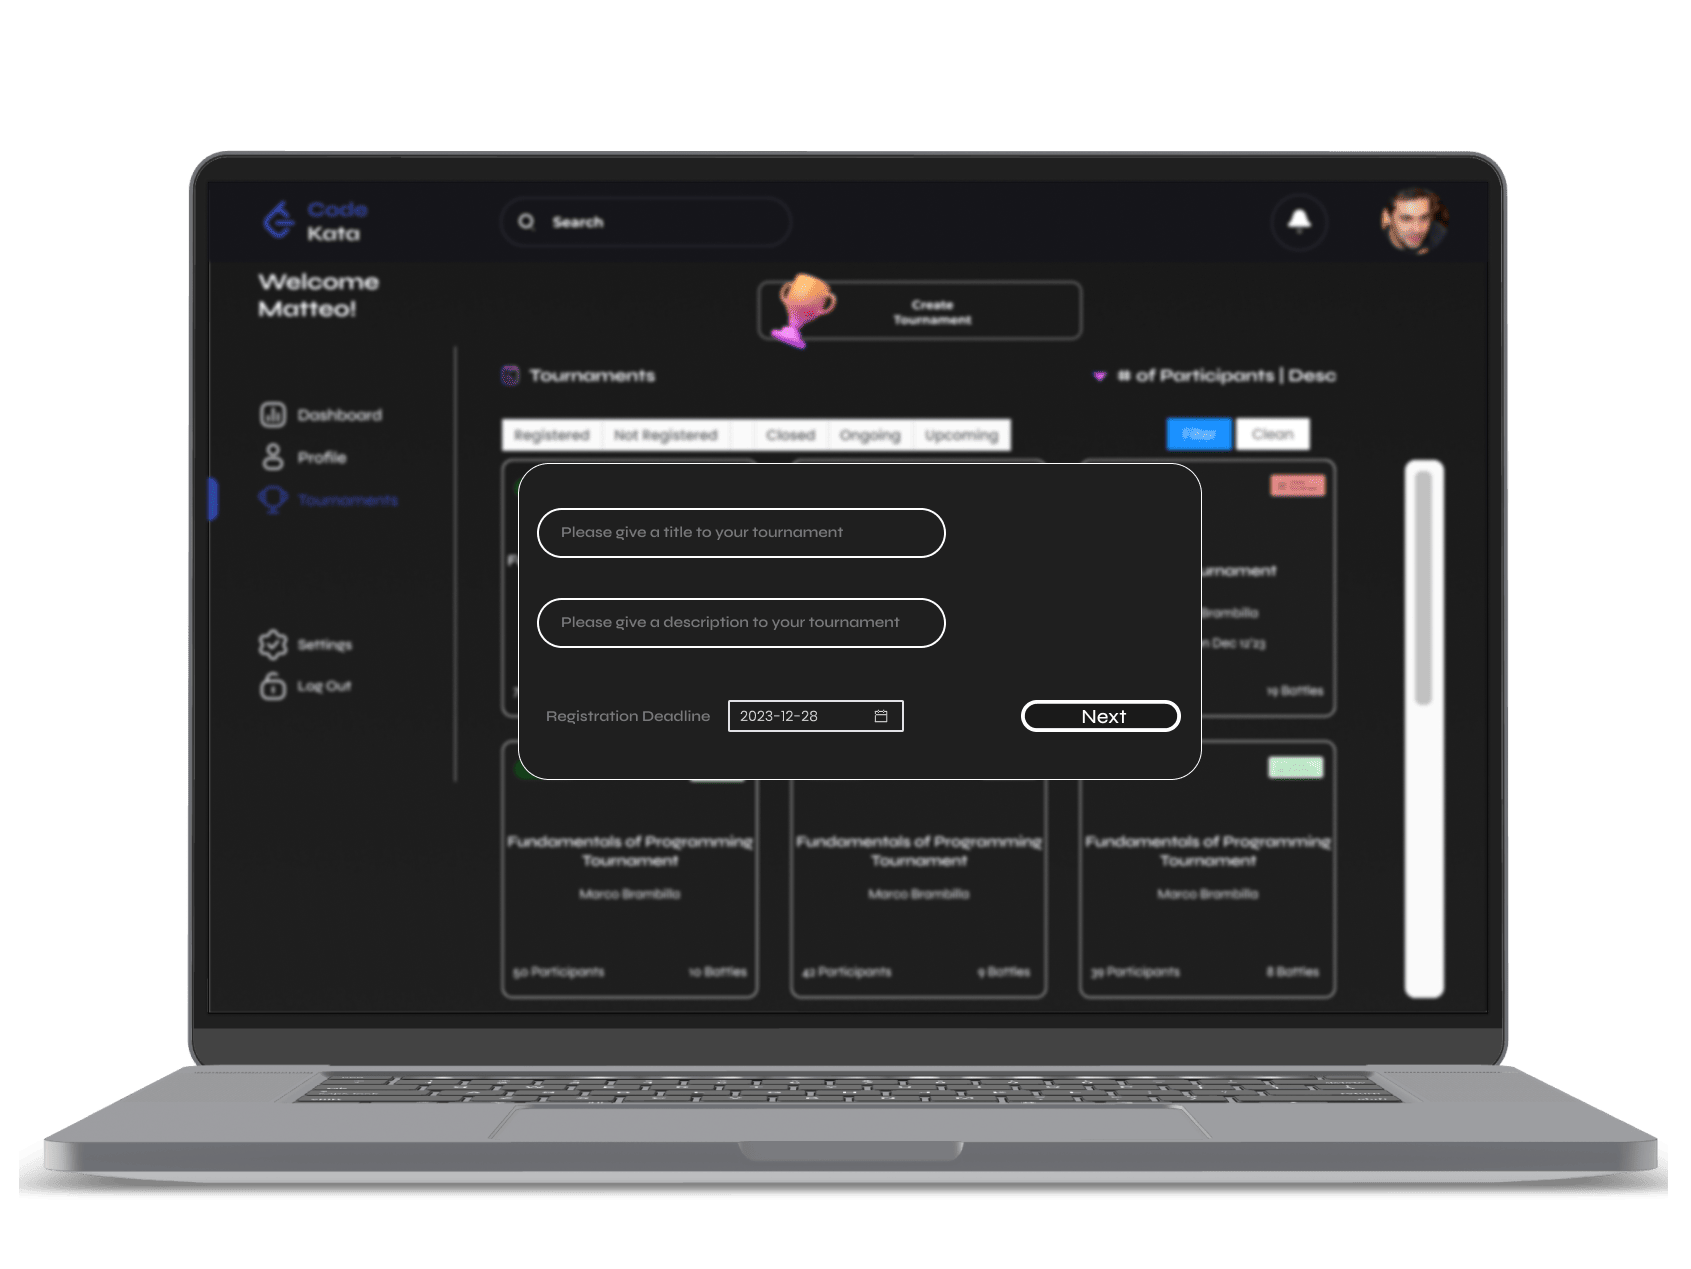
\includegraphics[scale=0.13]{Images/ui-ux/educator_create_tournament/educator_create_tournament_1.png}
% 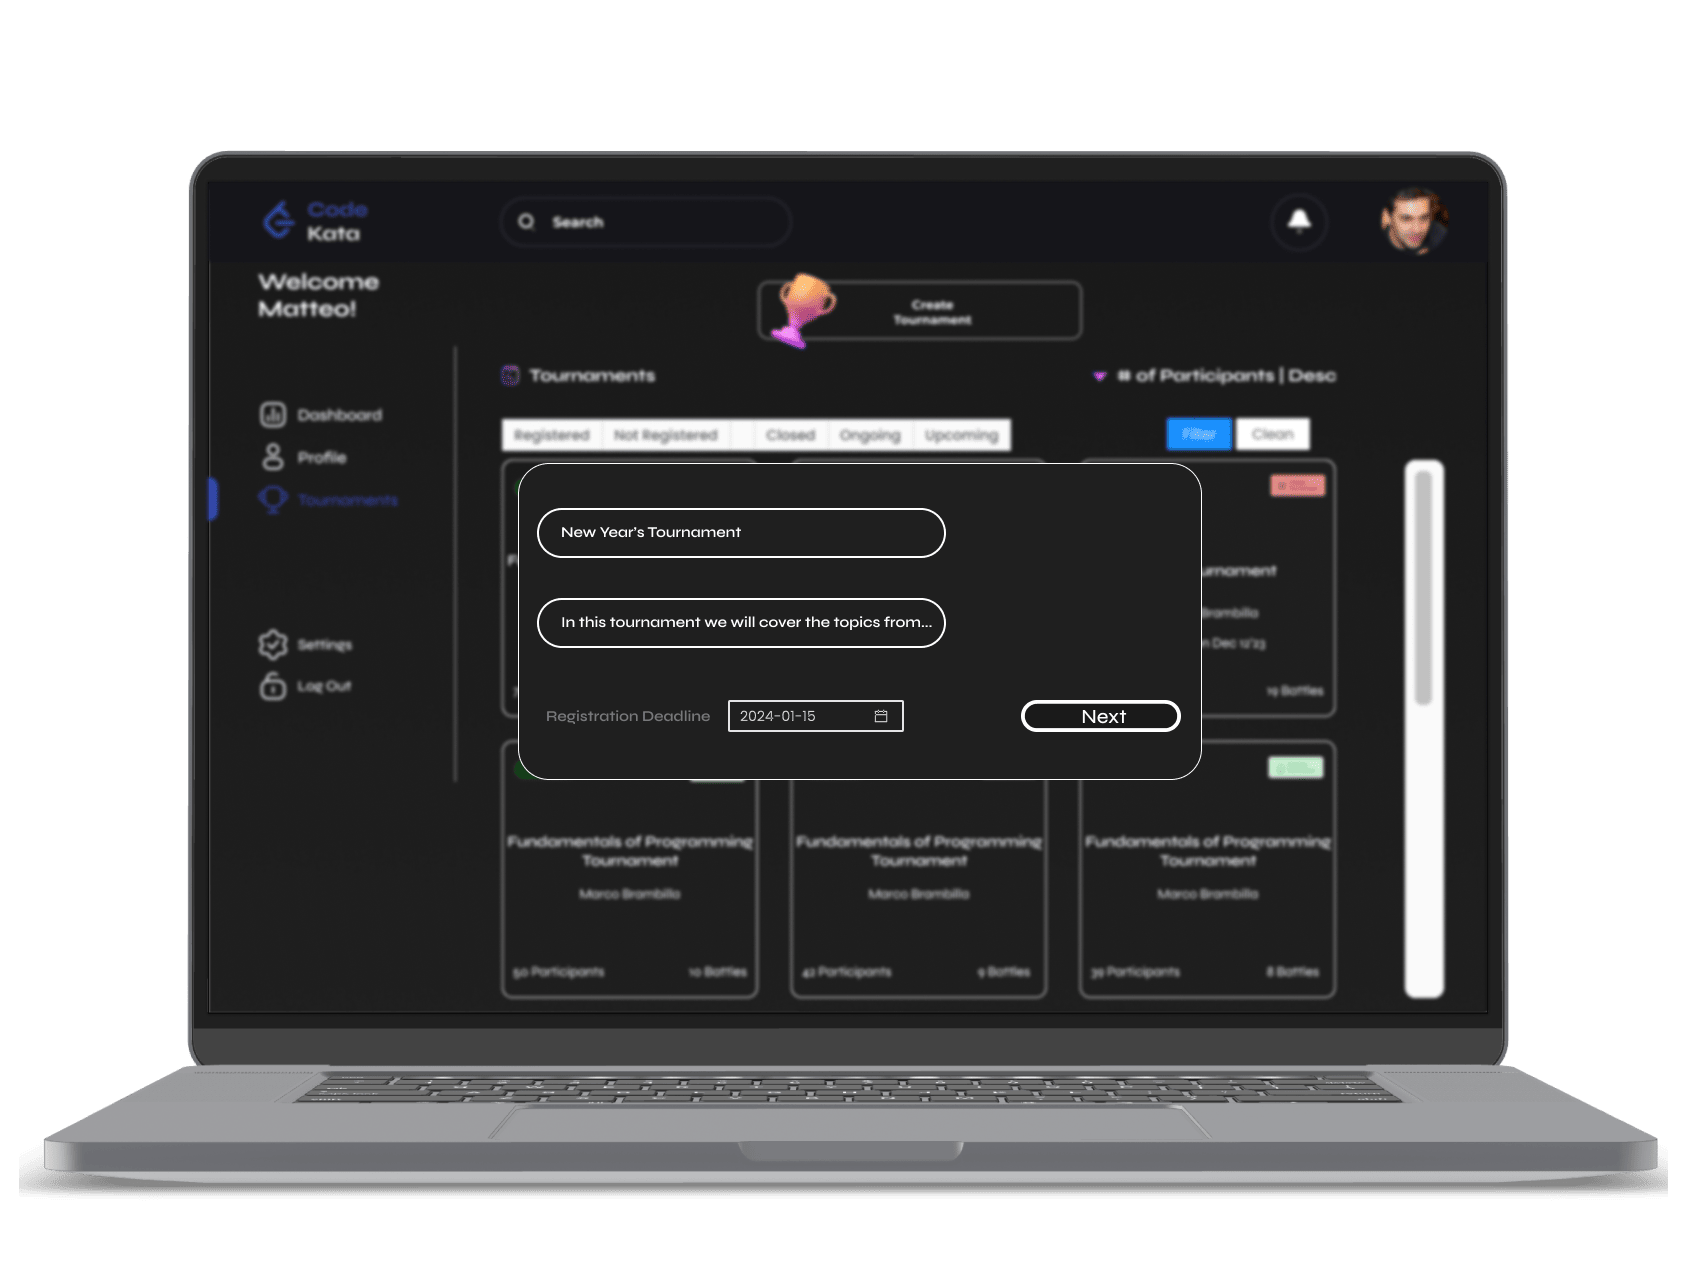
\includegraphics[scale=0.13]{Images/ui-ux/educator_create_tournament/educator_create_tournament_2.png}
% 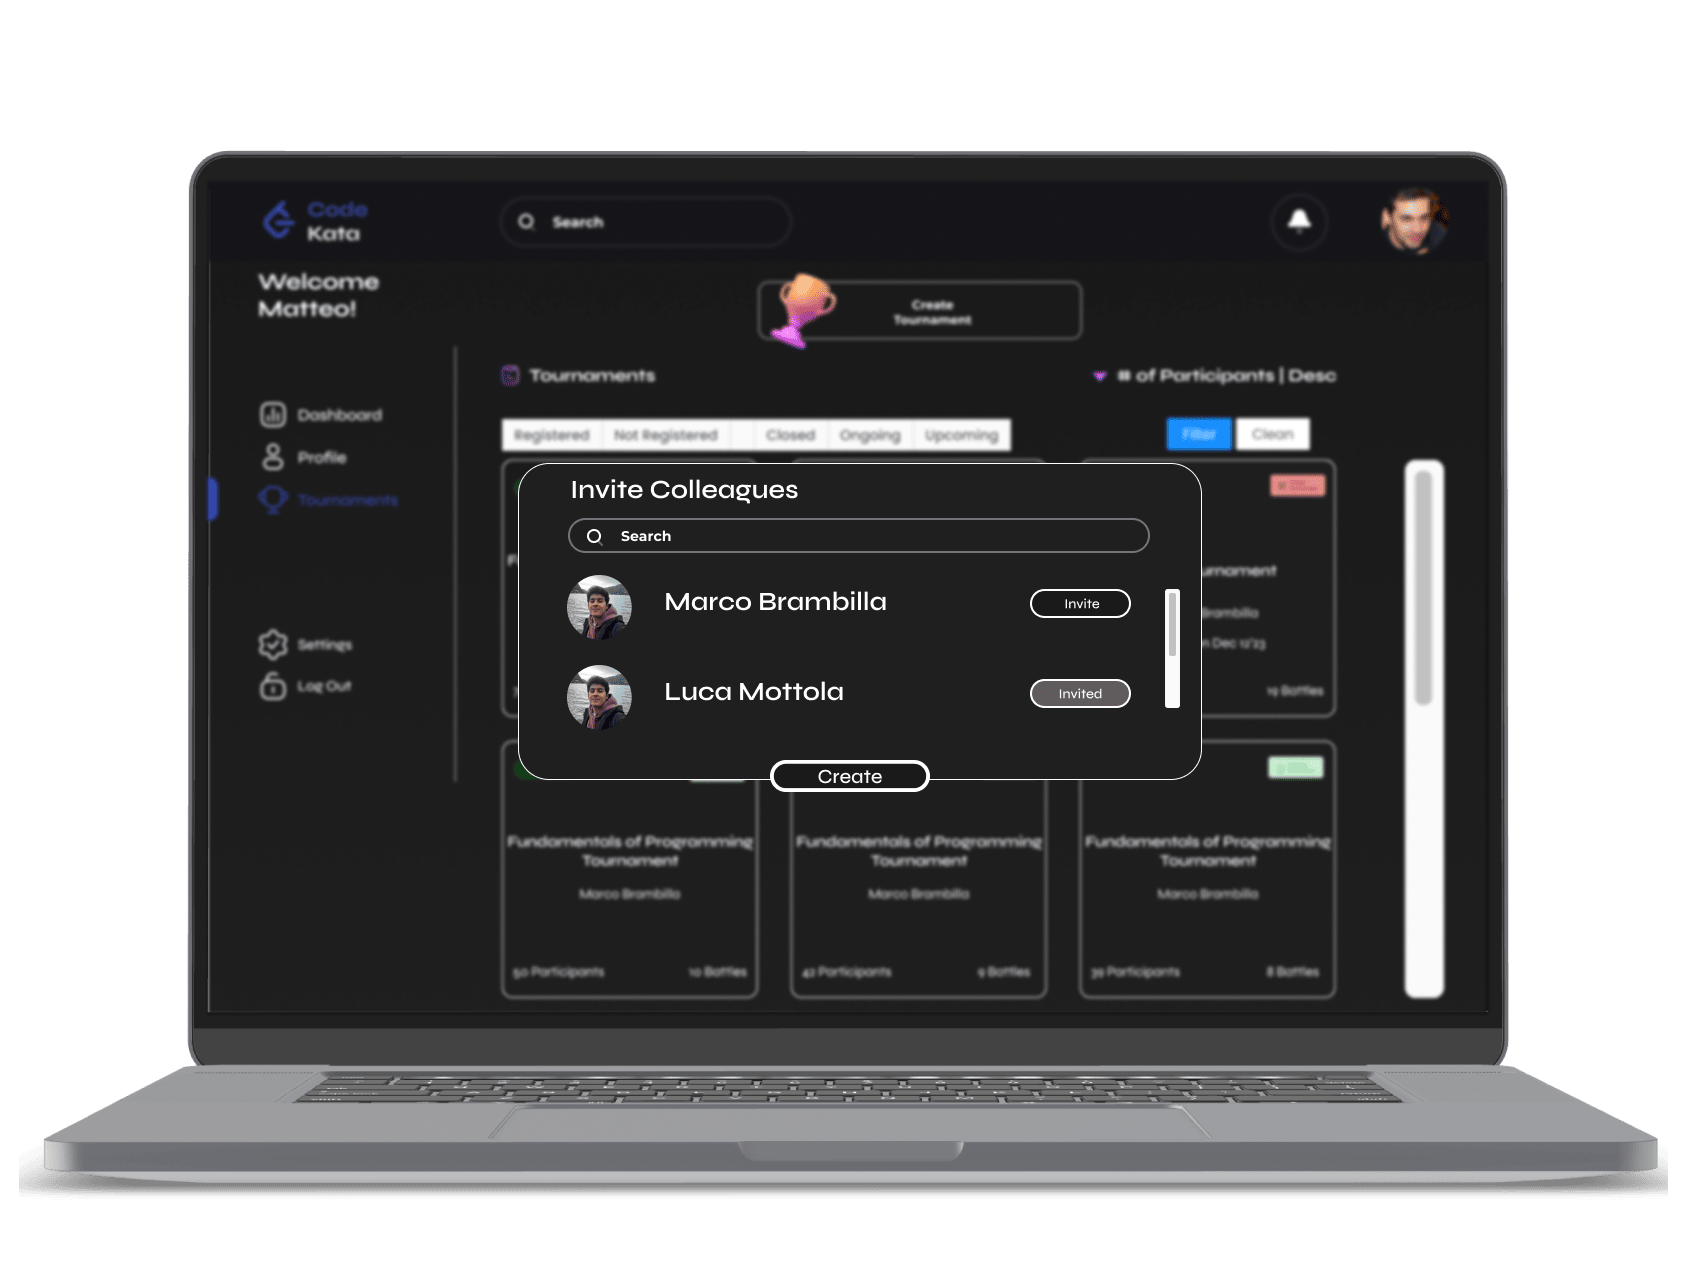
\includegraphics[scale=0.13]{Images/ui-ux/educator_create_tournament/educator_create_tournament_3.png}
% 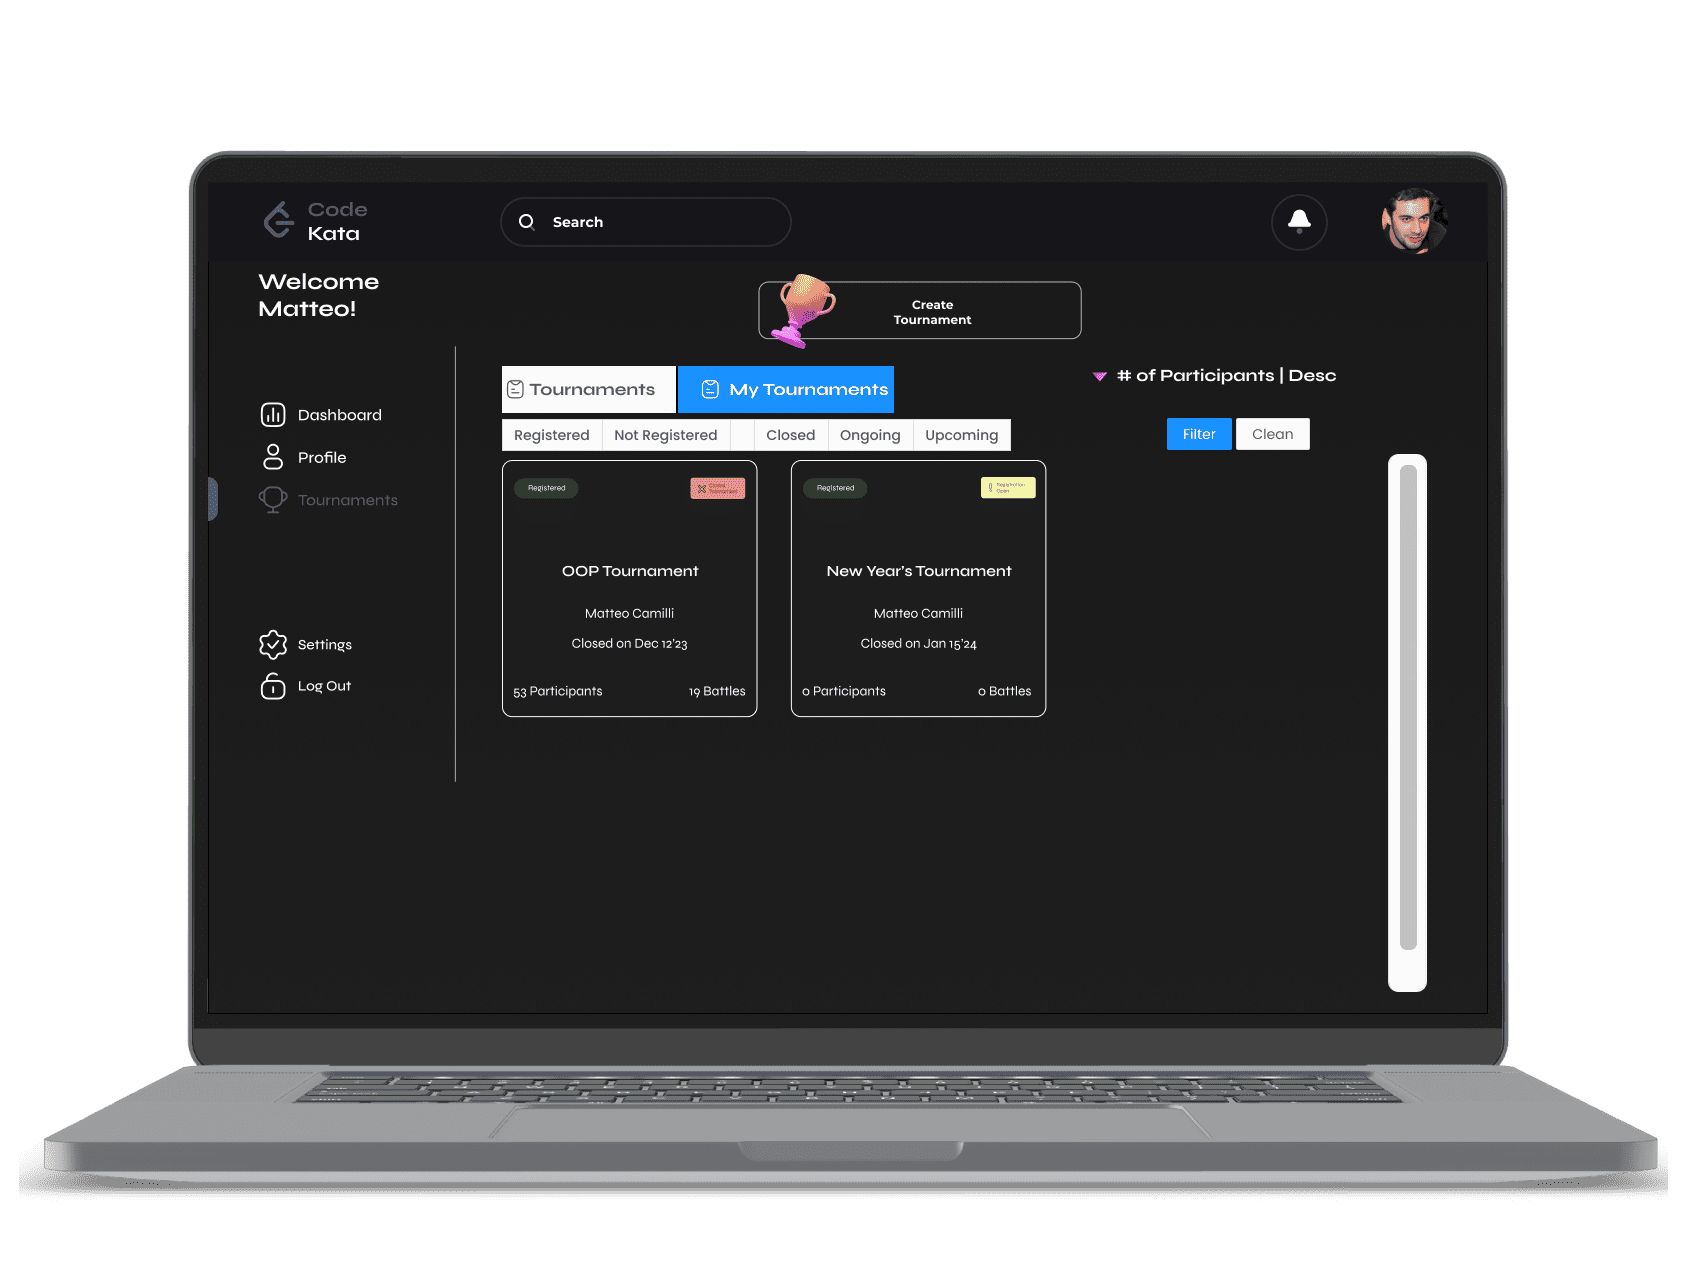
\includegraphics[scale=0.13]{Images/ui-ux/educator_create_tournament/educator_create_tournament_4.png}
%         (a) Educator Creates Tournaments
% \end{center}
% \begin{center}
% 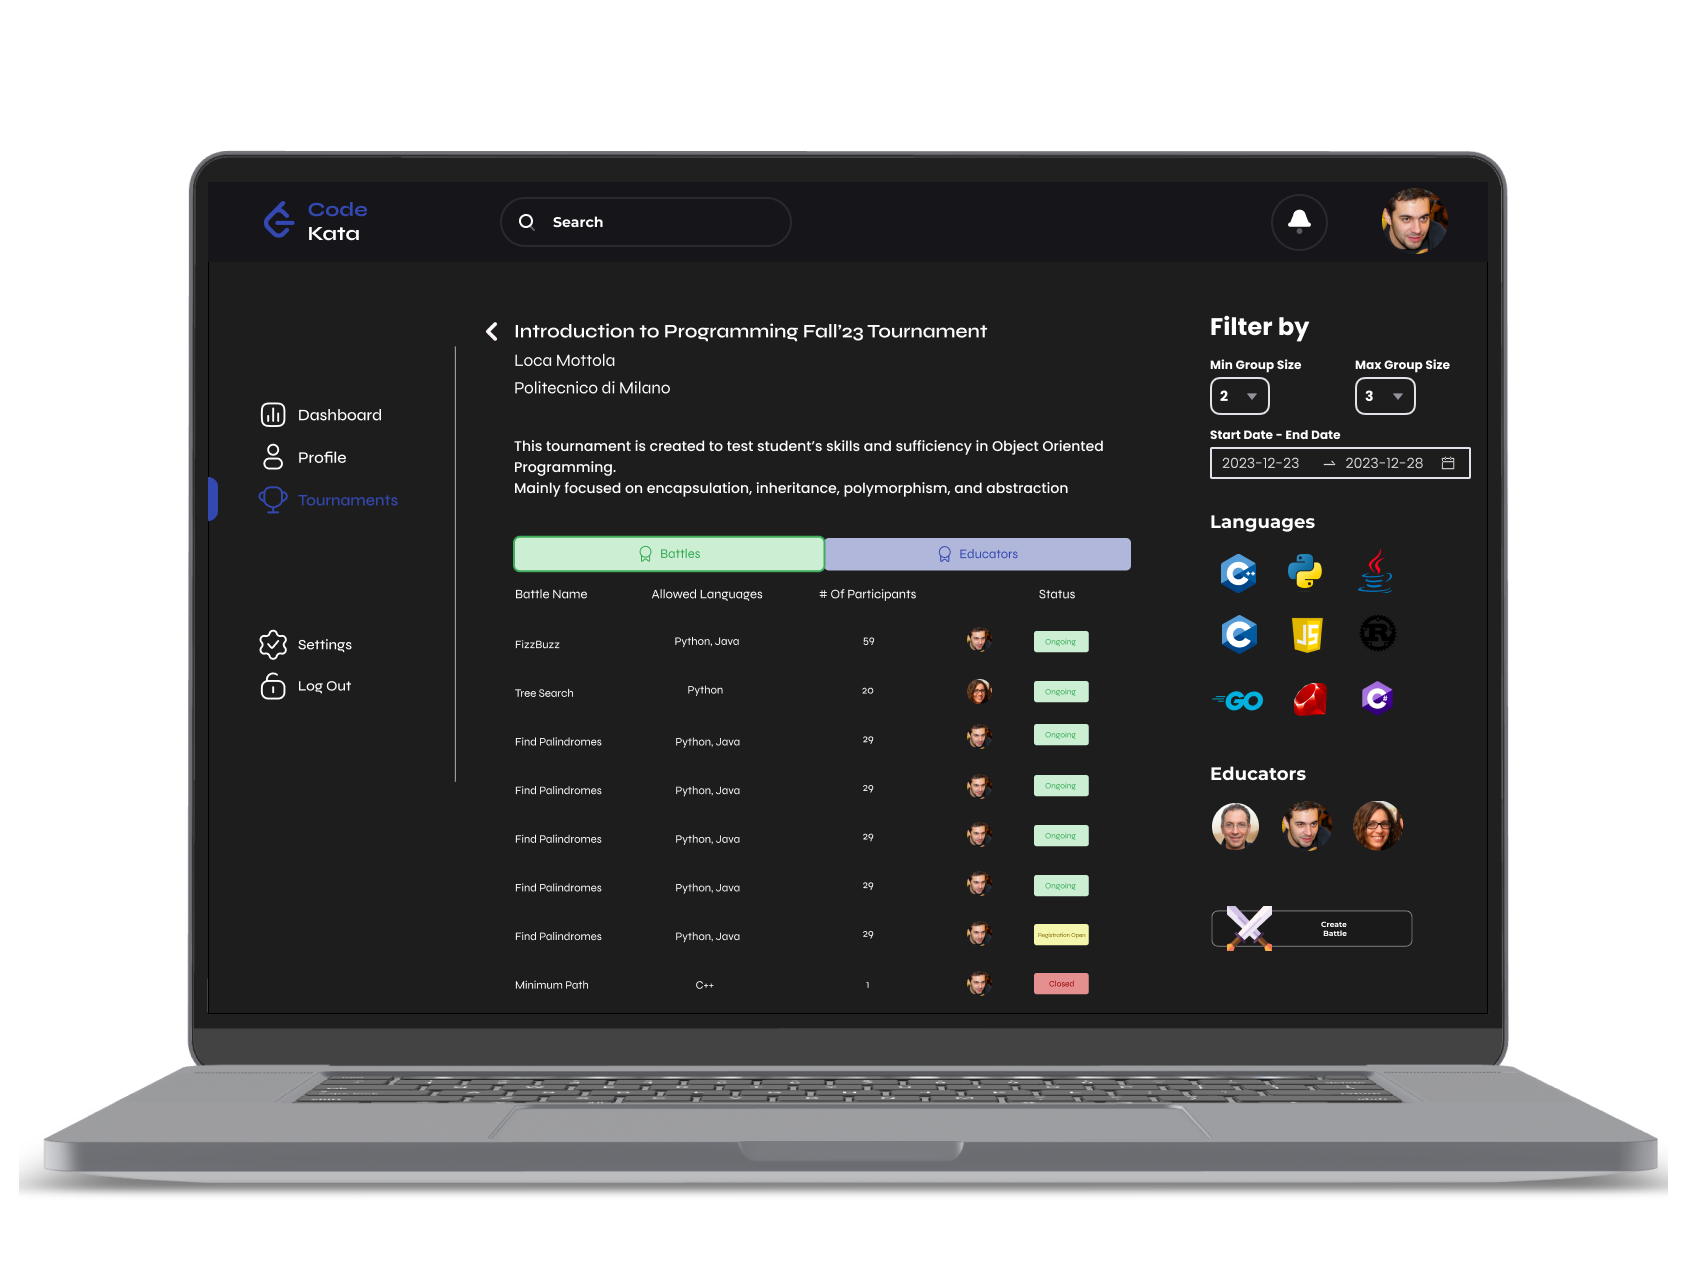
\includegraphics[scale=0.13]{Images/ui-ux/educator_creates_battle/educator_creates_battle_1.png}
% 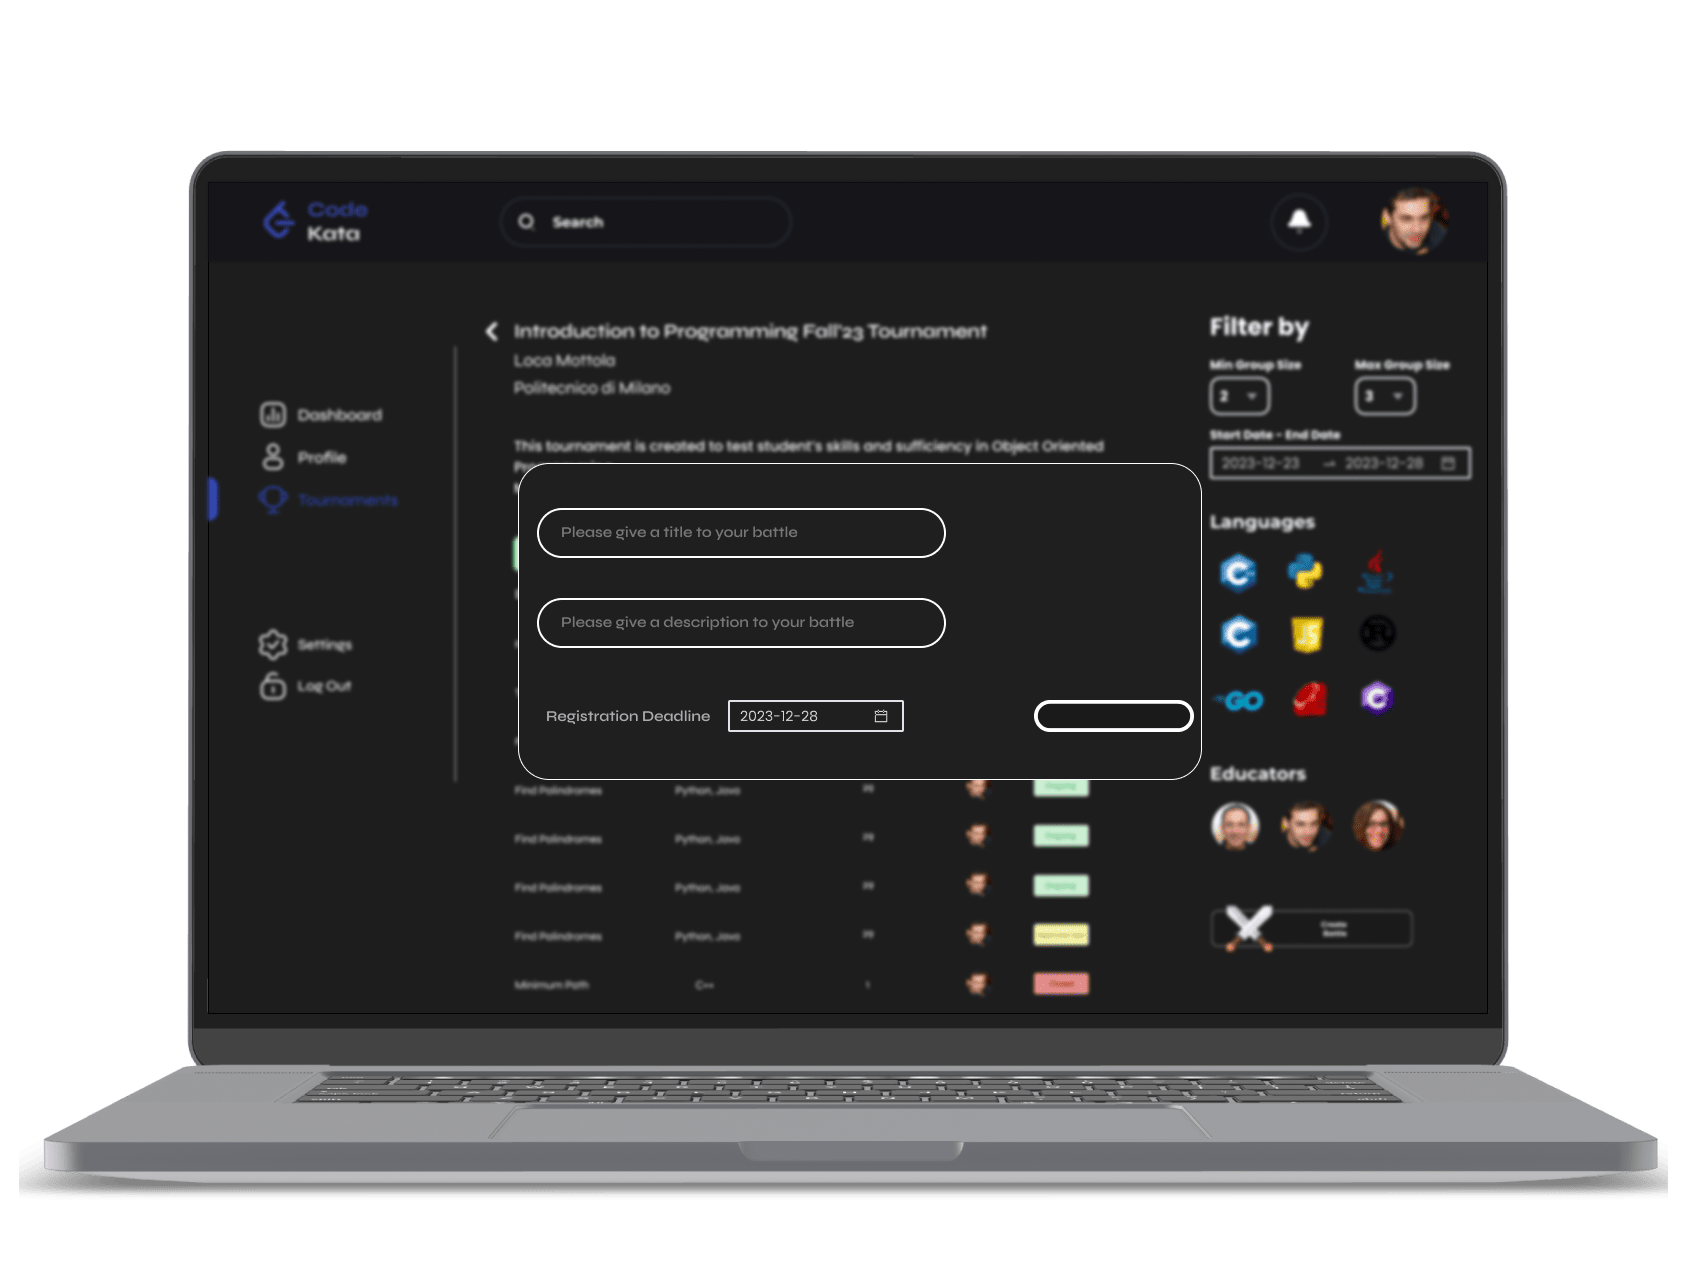
\includegraphics[scale=0.13]{Images/ui-ux/educator_creates_battle/educator_creates_battle_2.png}
% 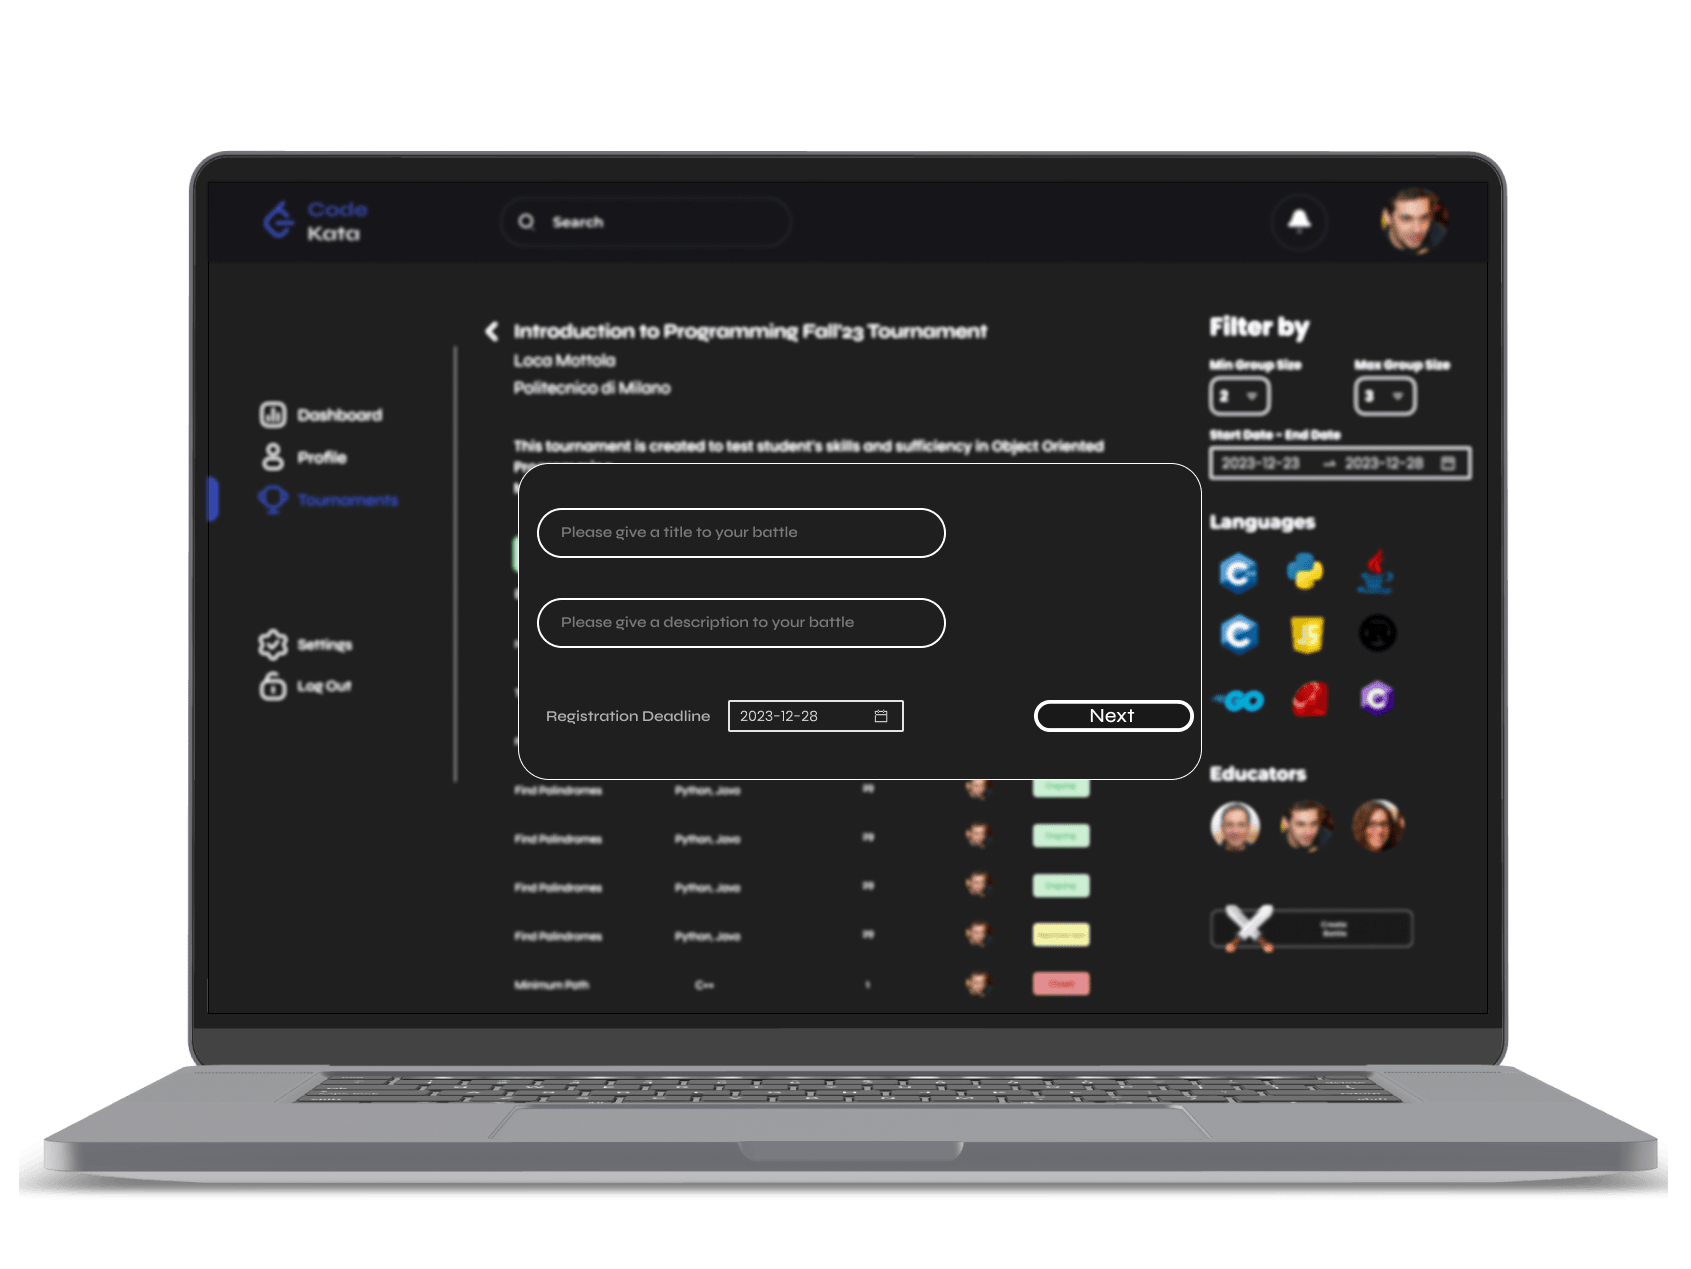
\includegraphics[scale=0.13]{Images/ui-ux/educator_creates_battle/educator_creates_battle_3.png}
% 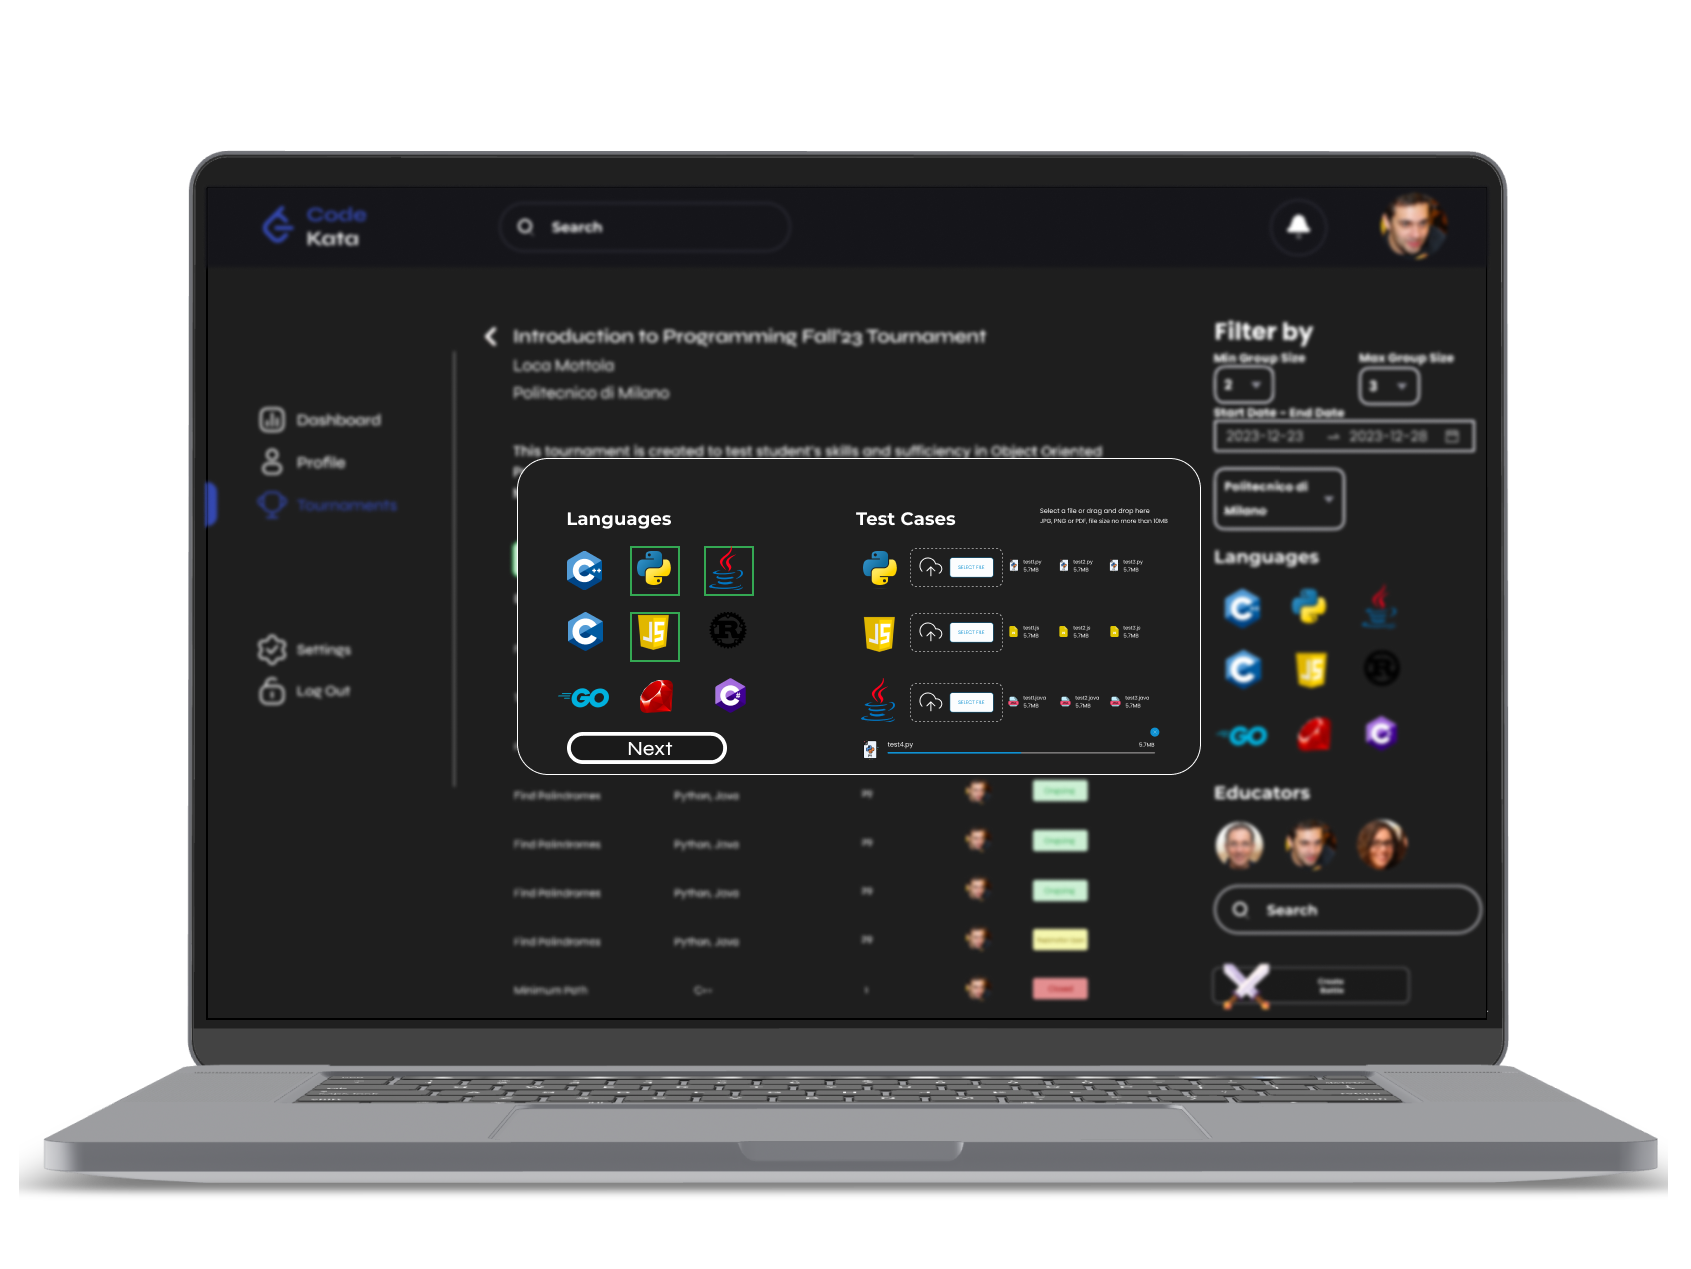
\includegraphics[scale=0.13]{Images/ui-ux/educator_creates_battle/educator_creates_battle_4.png}
% 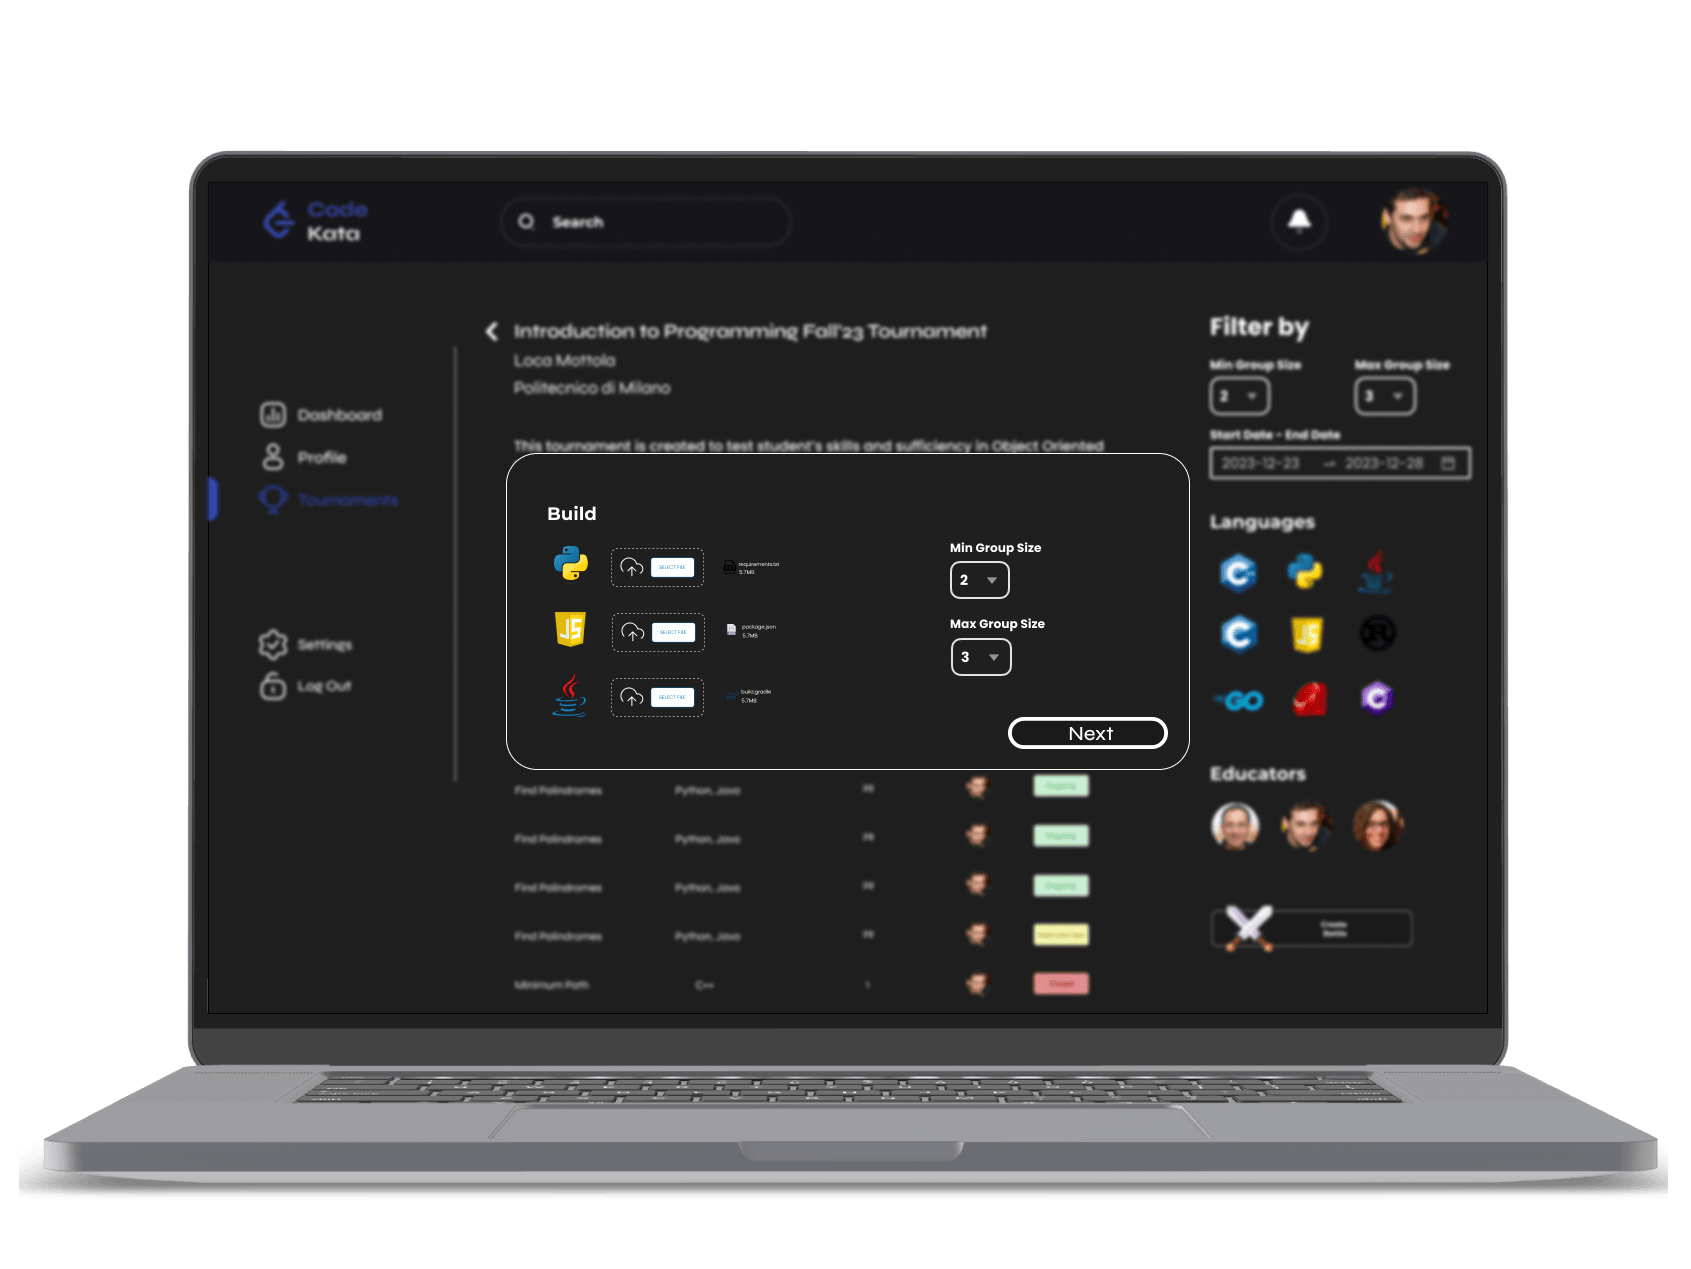
\includegraphics[scale=0.13]{Images/ui-ux/educator_creates_battle/educator_creates_battle_5.png}
% 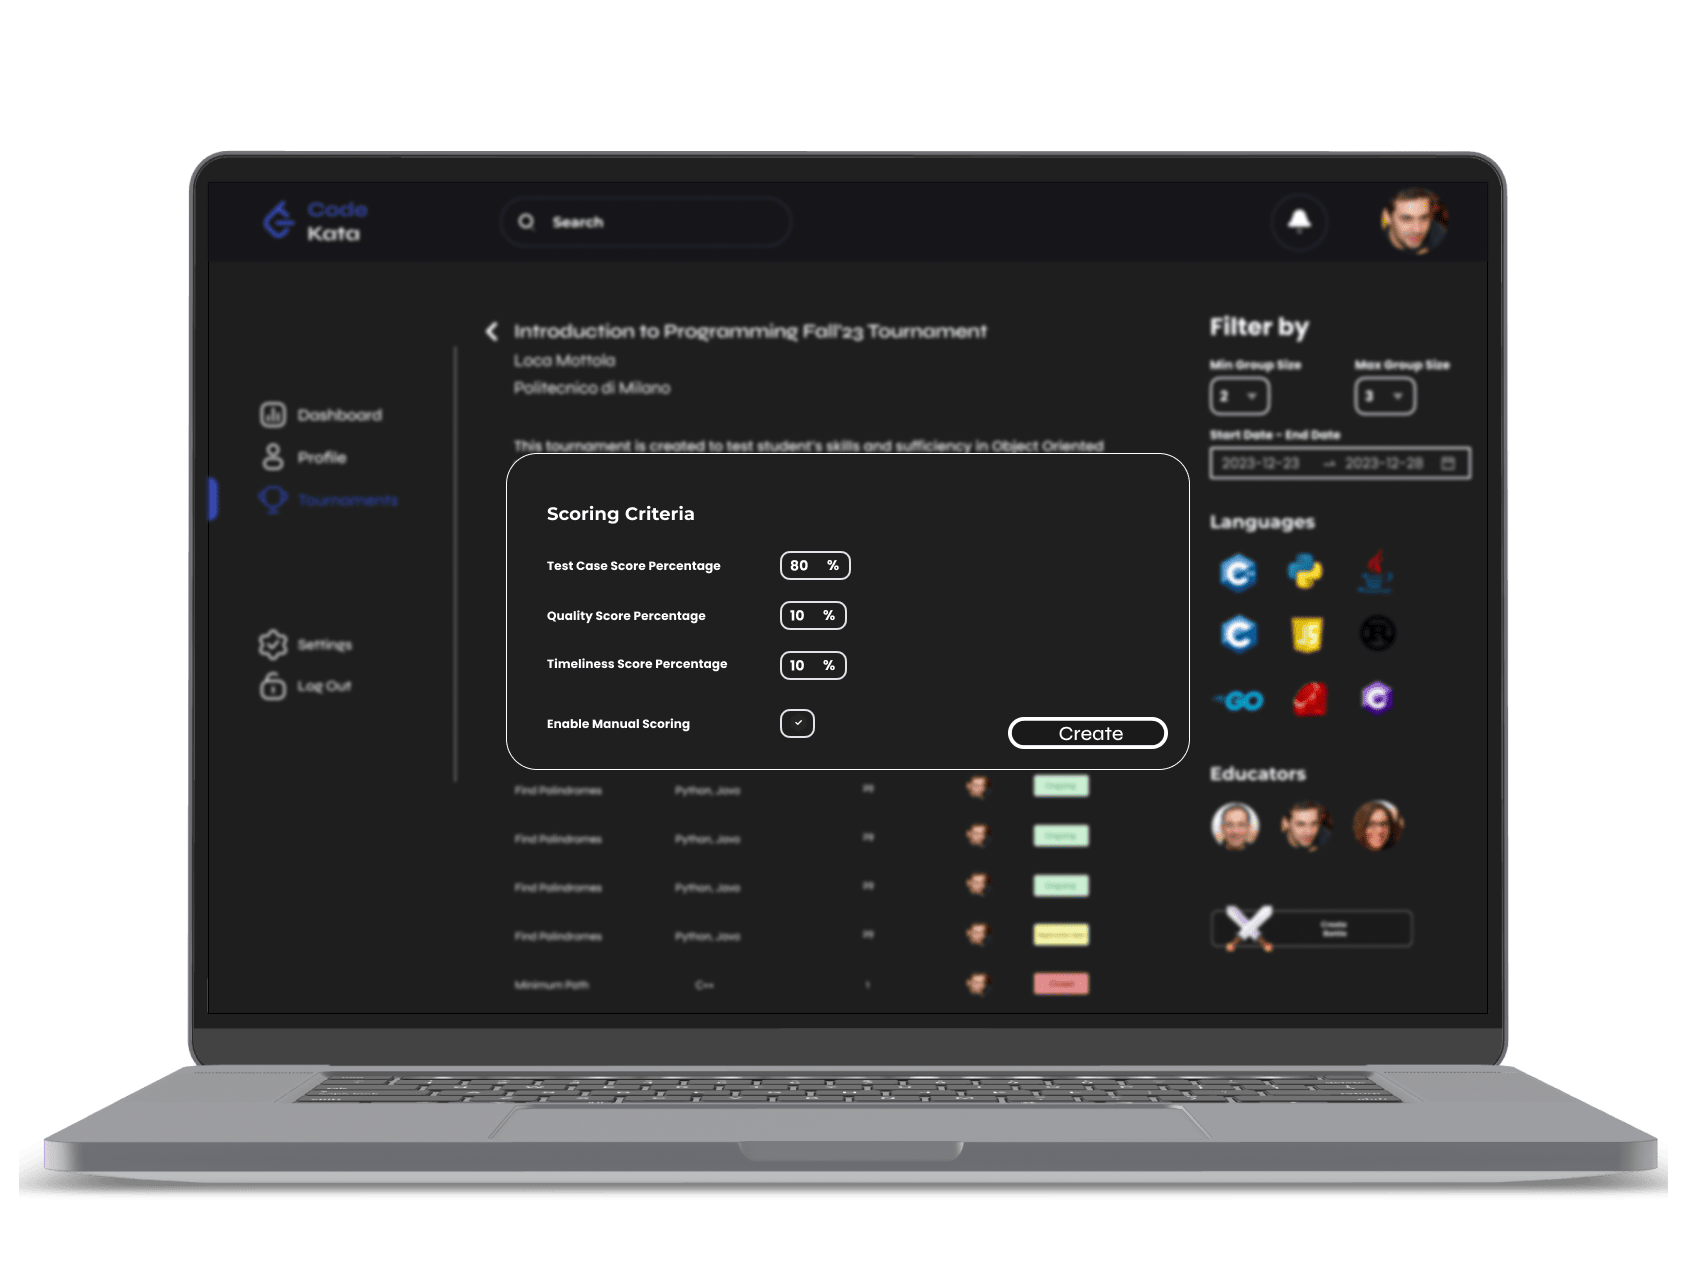
\includegraphics[scale=0.13]{Images/ui-ux/educator_creates_battle/educator_creates_battle_6.png}
%         (a) Educator Creates Battle
% \end{center}
% \begin{center}
% 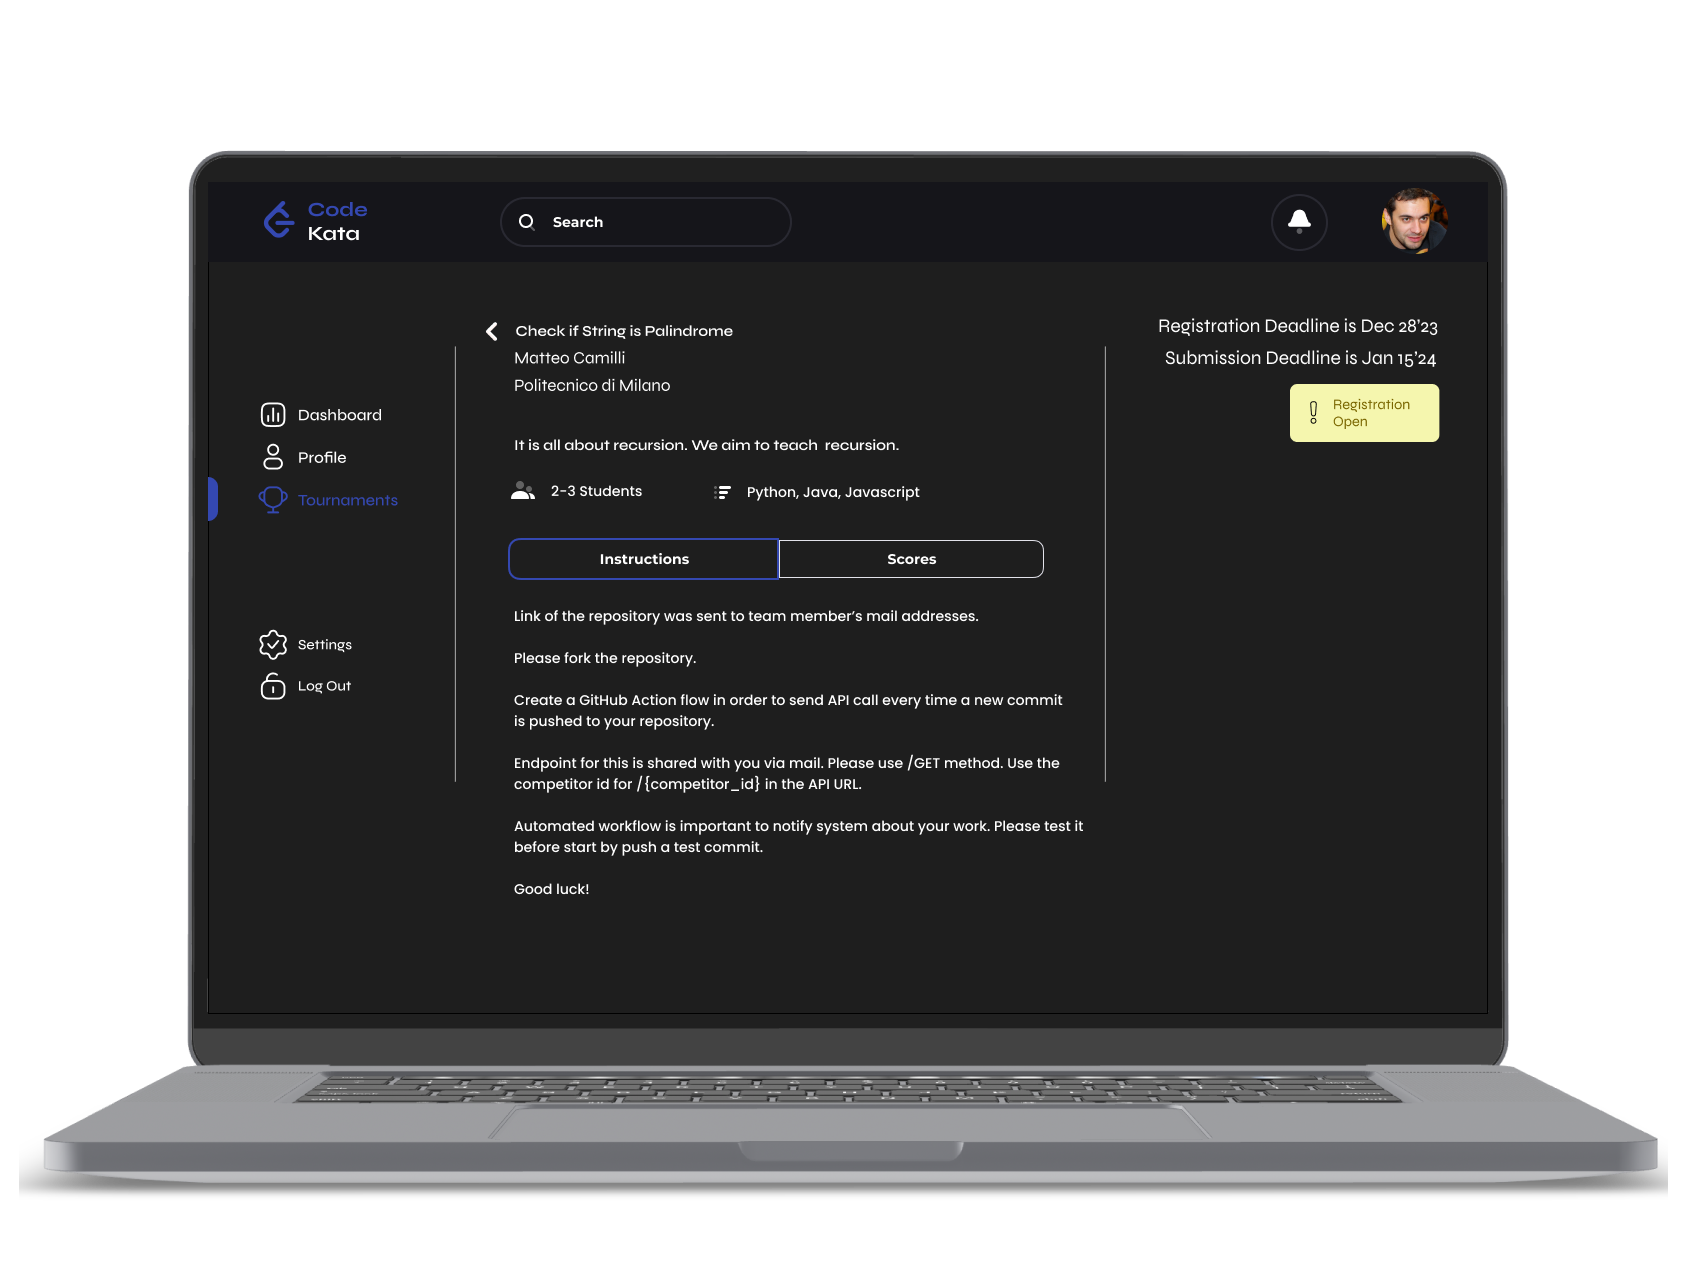
\includegraphics[scale=0.13]{Images/ui-ux/educator_battle/educator_battle_1.png}
% 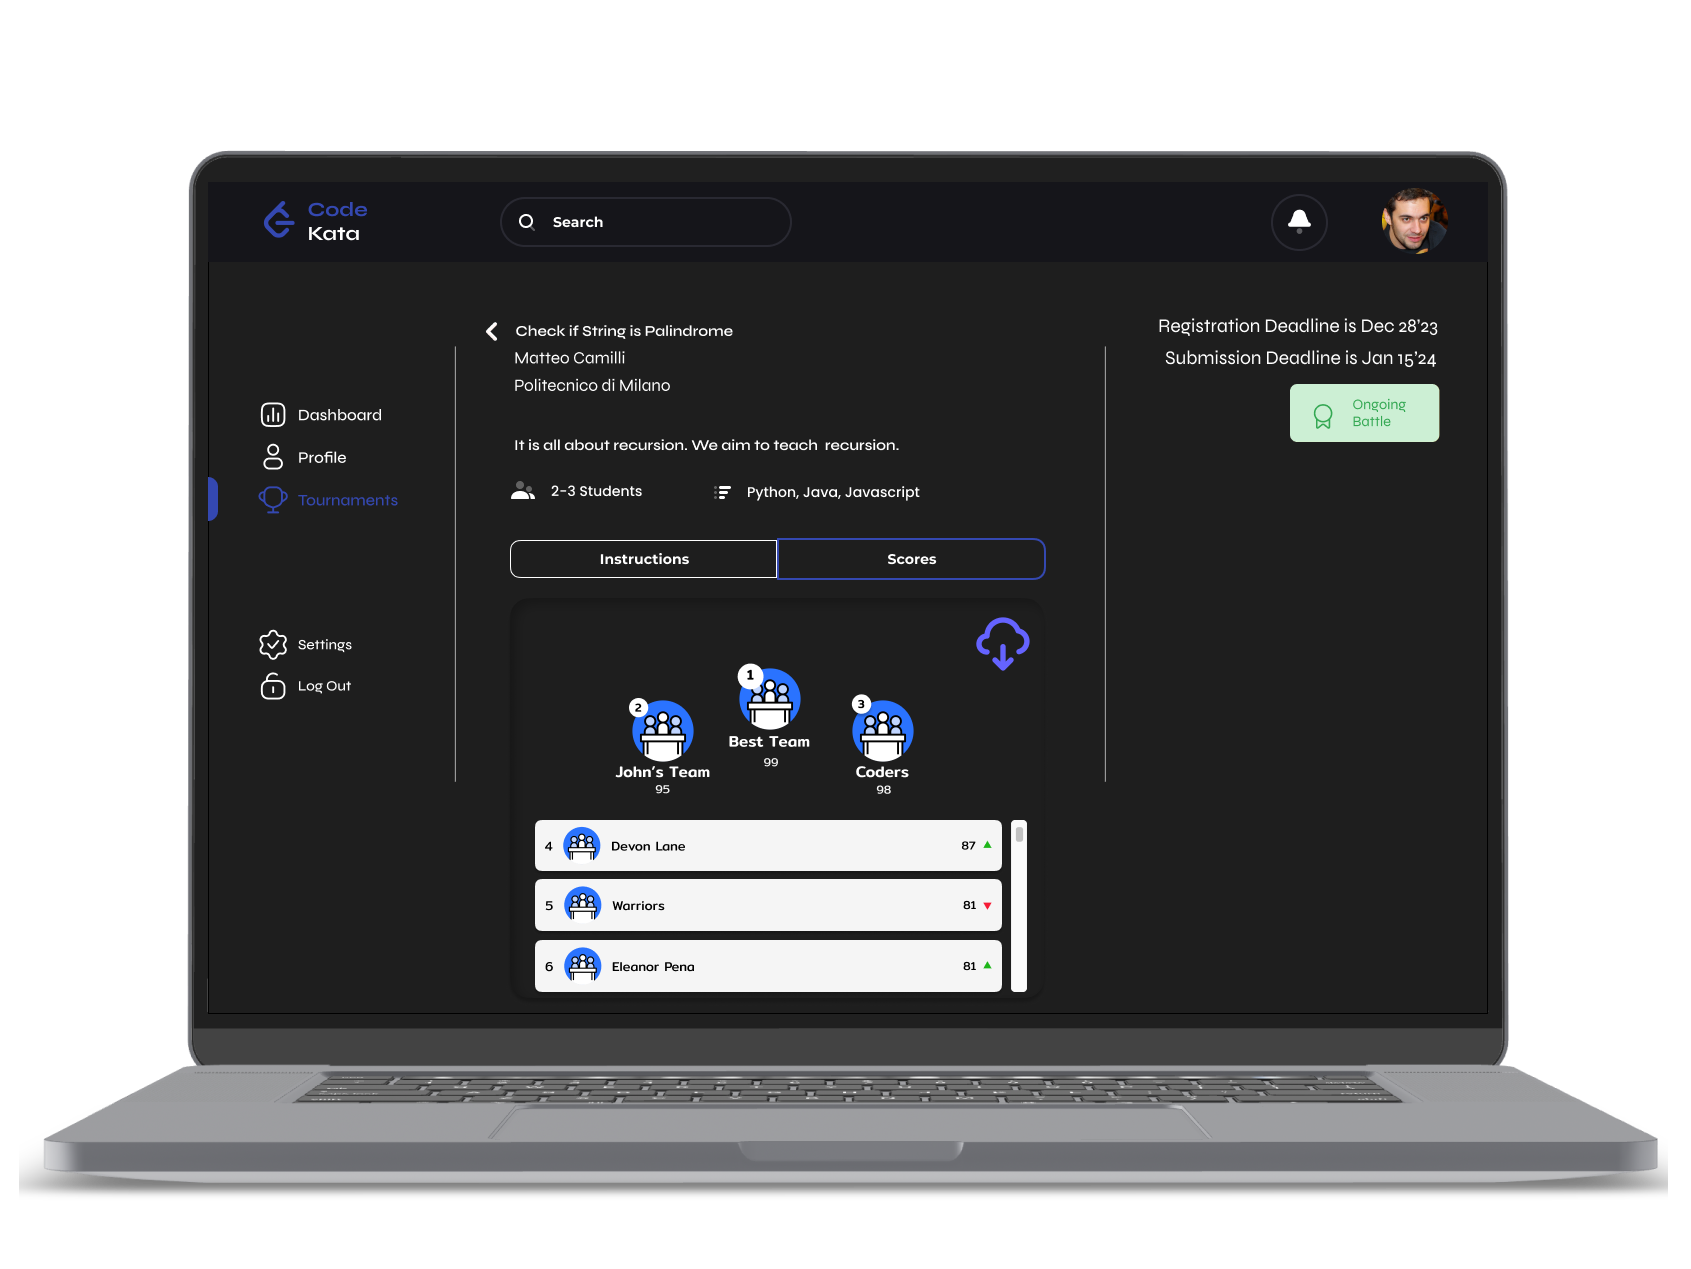
\includegraphics[scale=0.13]{Images/ui-ux/educator_battle/educator_battle_2.png}
% 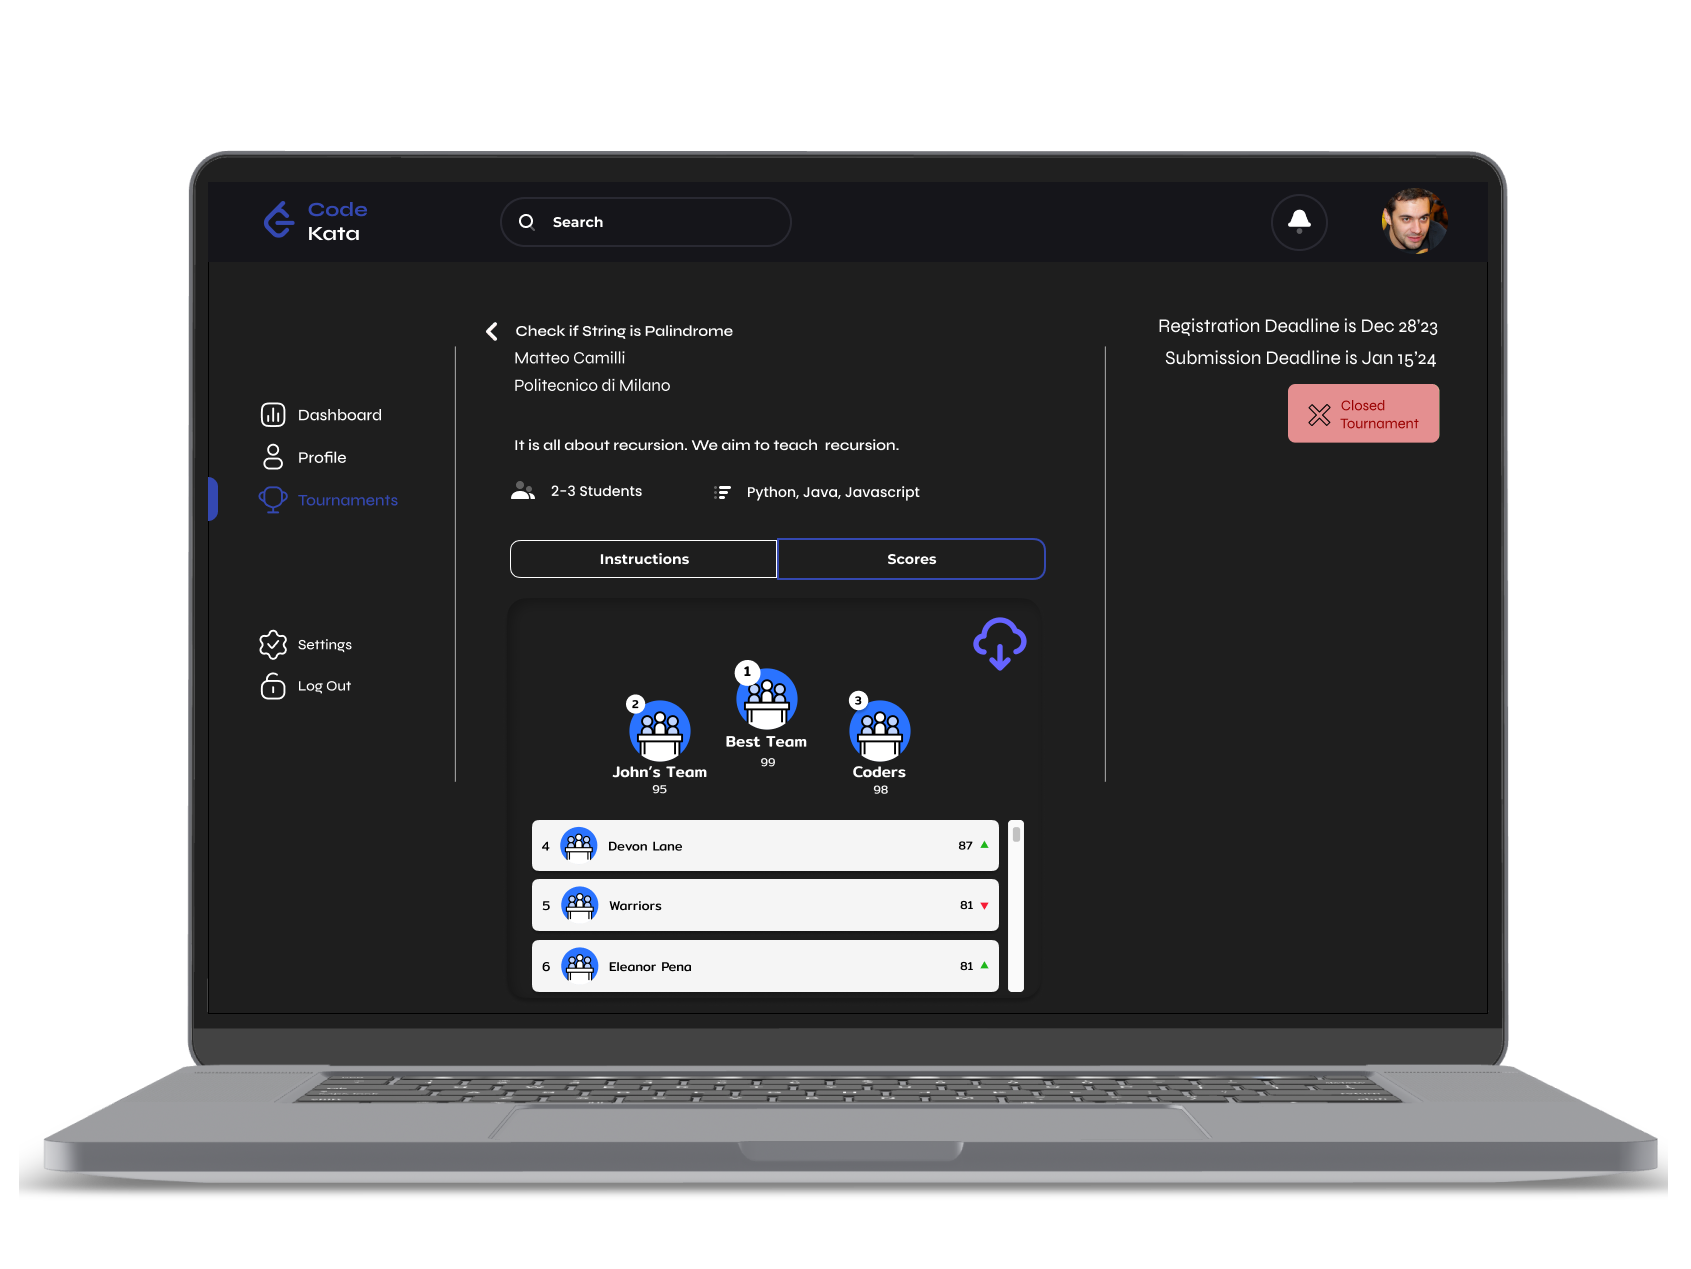
\includegraphics[scale=0.13]{Images/ui-ux/educator_battle/educator_battle_3.png}
%  \\(a) Educator and Battle
% \end{center}
% \begin{center}
% 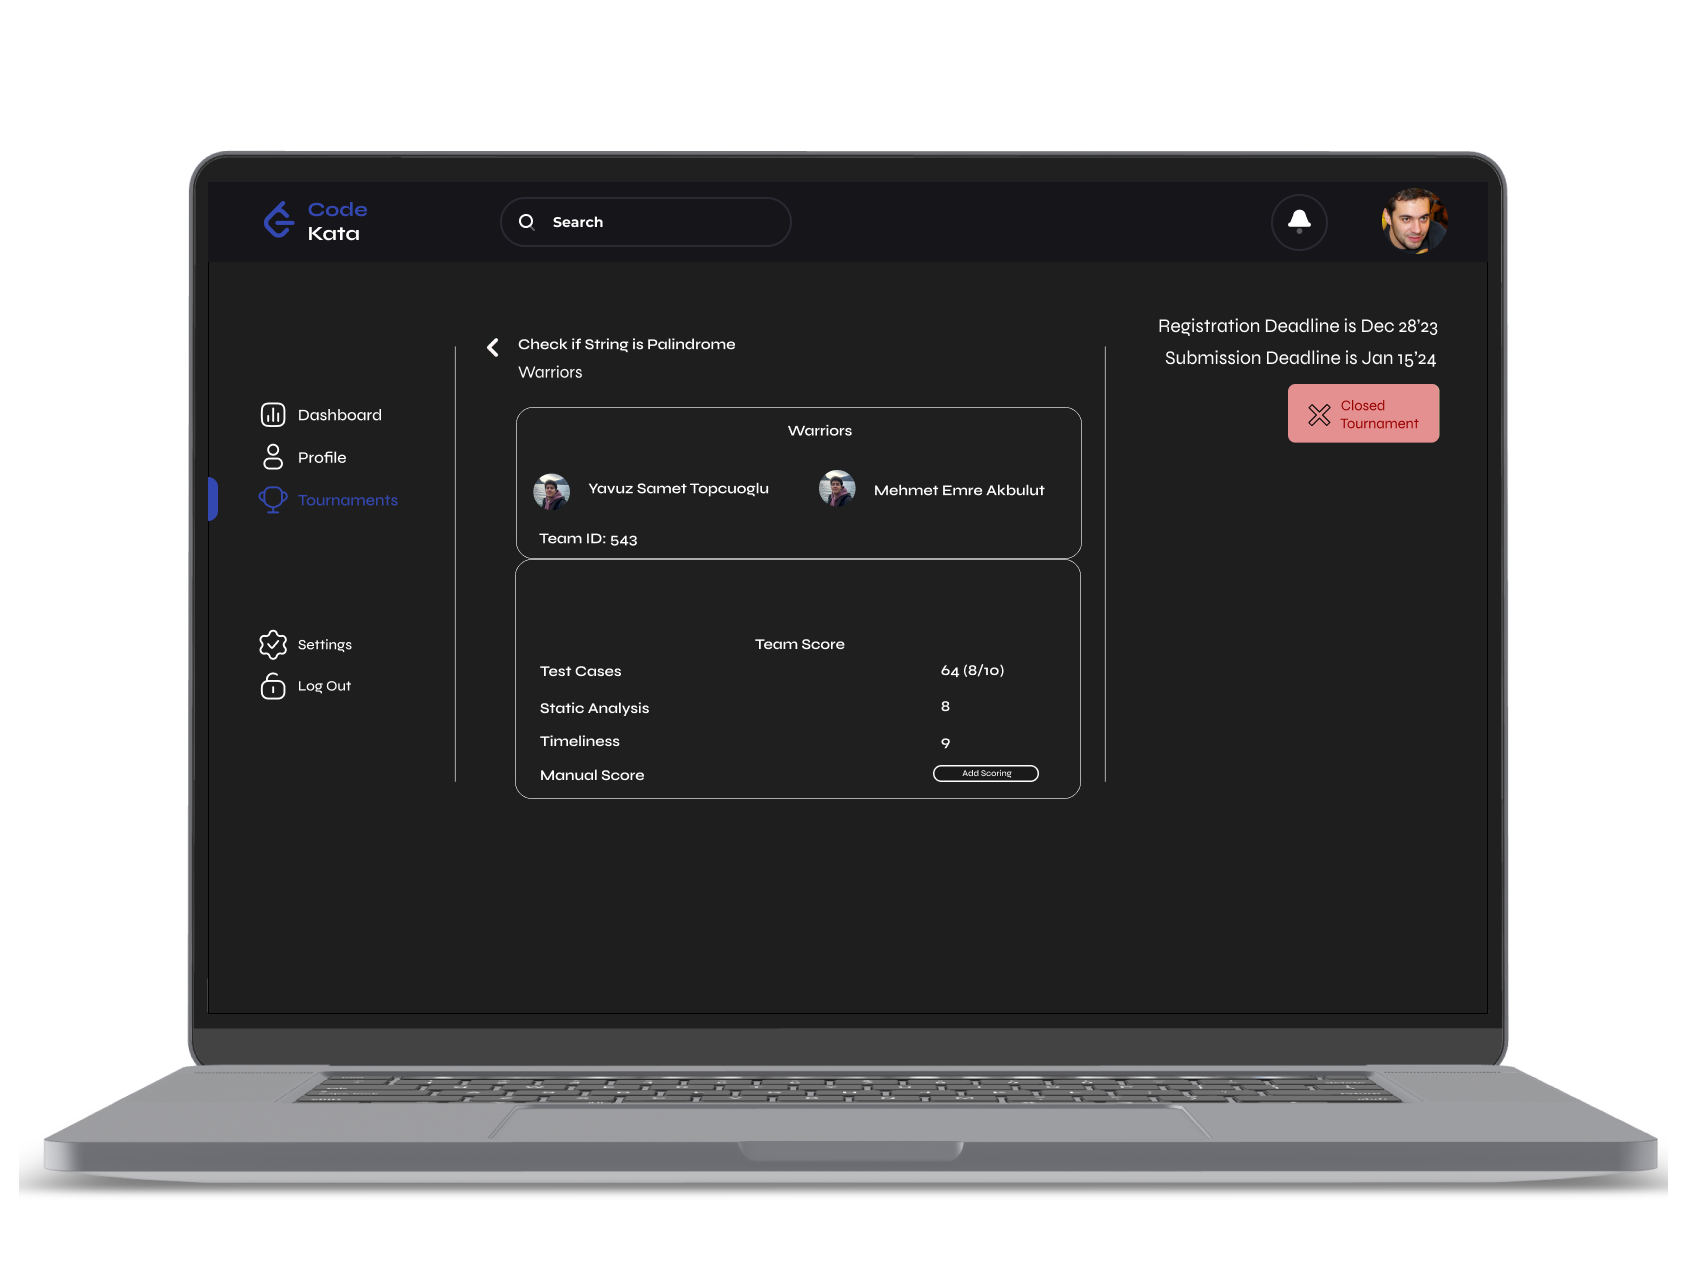
\includegraphics[scale=0.13]{Images/ui-ux/educator_team/educator_team_1.png}
% 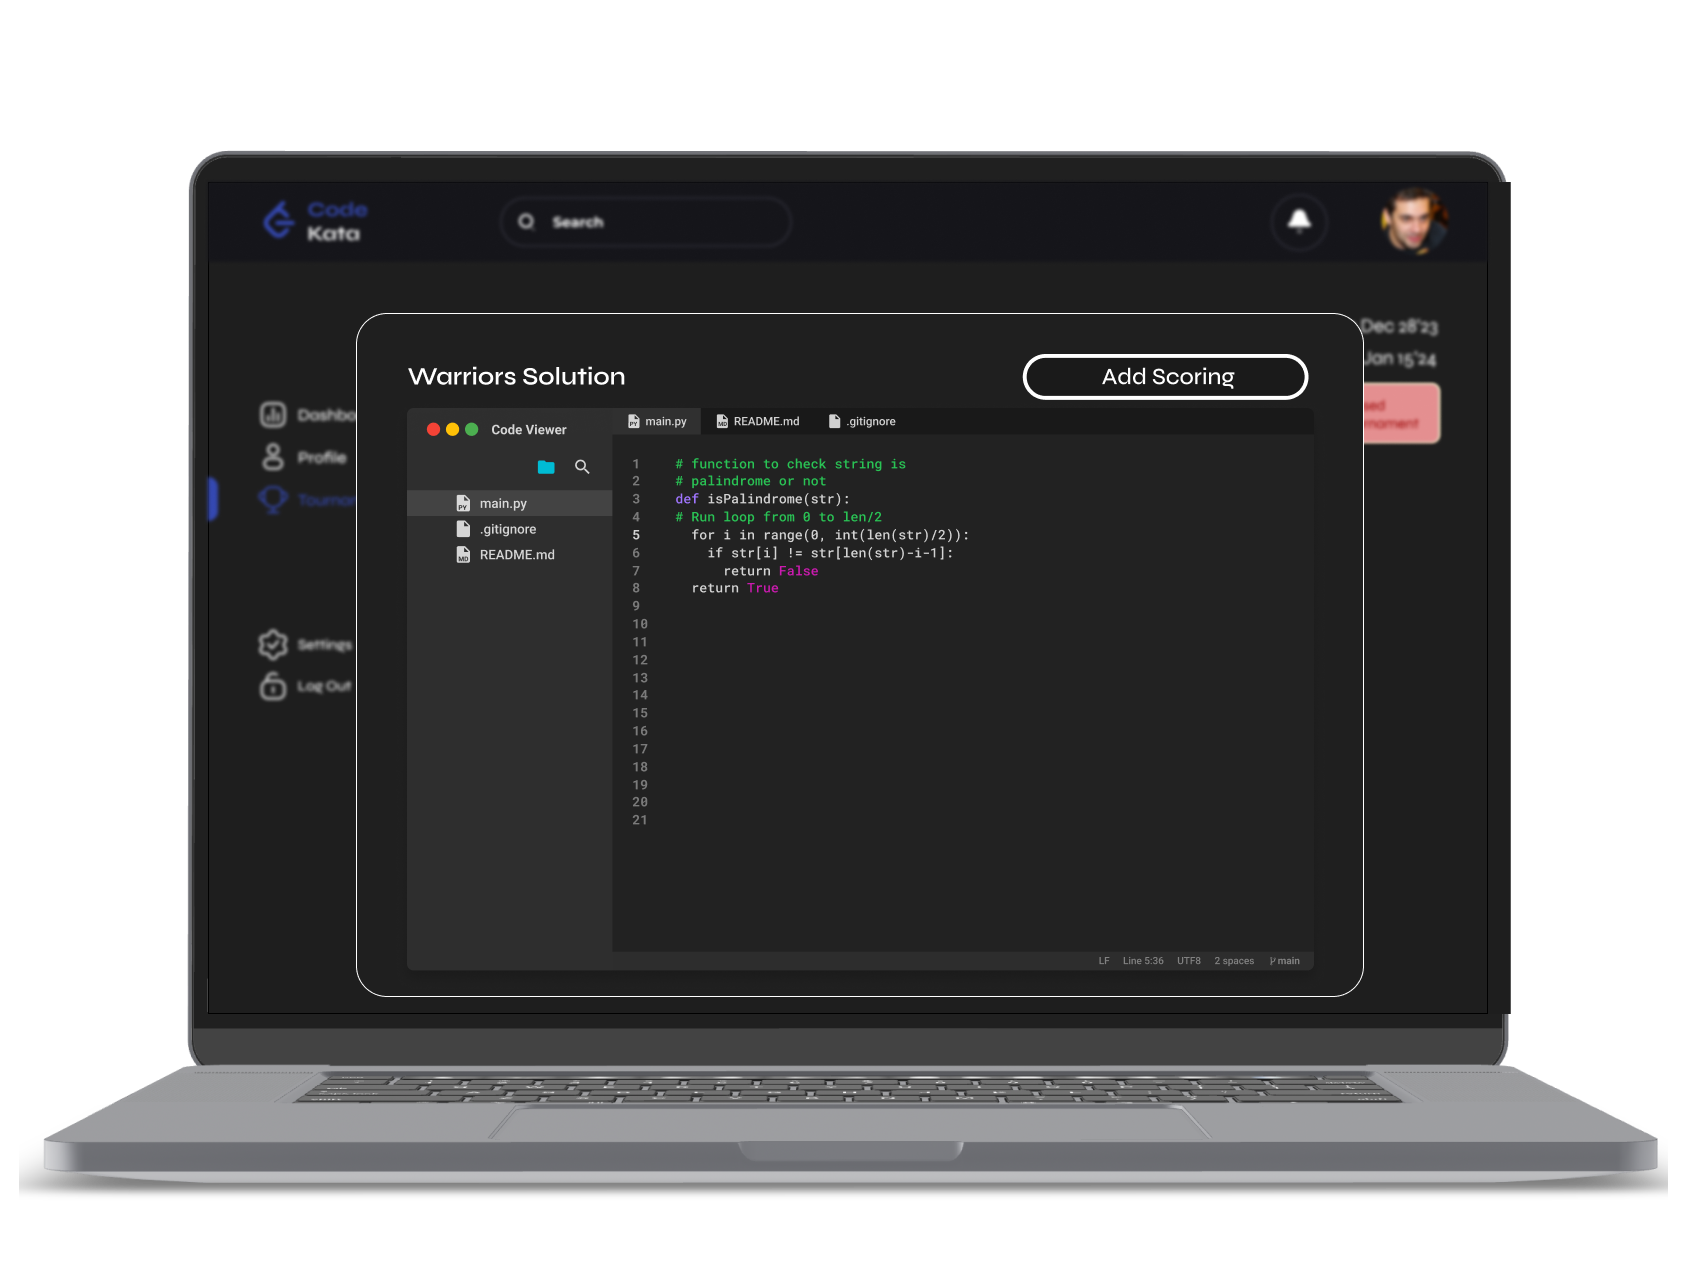
\includegraphics[scale=0.13]{Images/ui-ux/educator_team/educator_team_2.png}
% 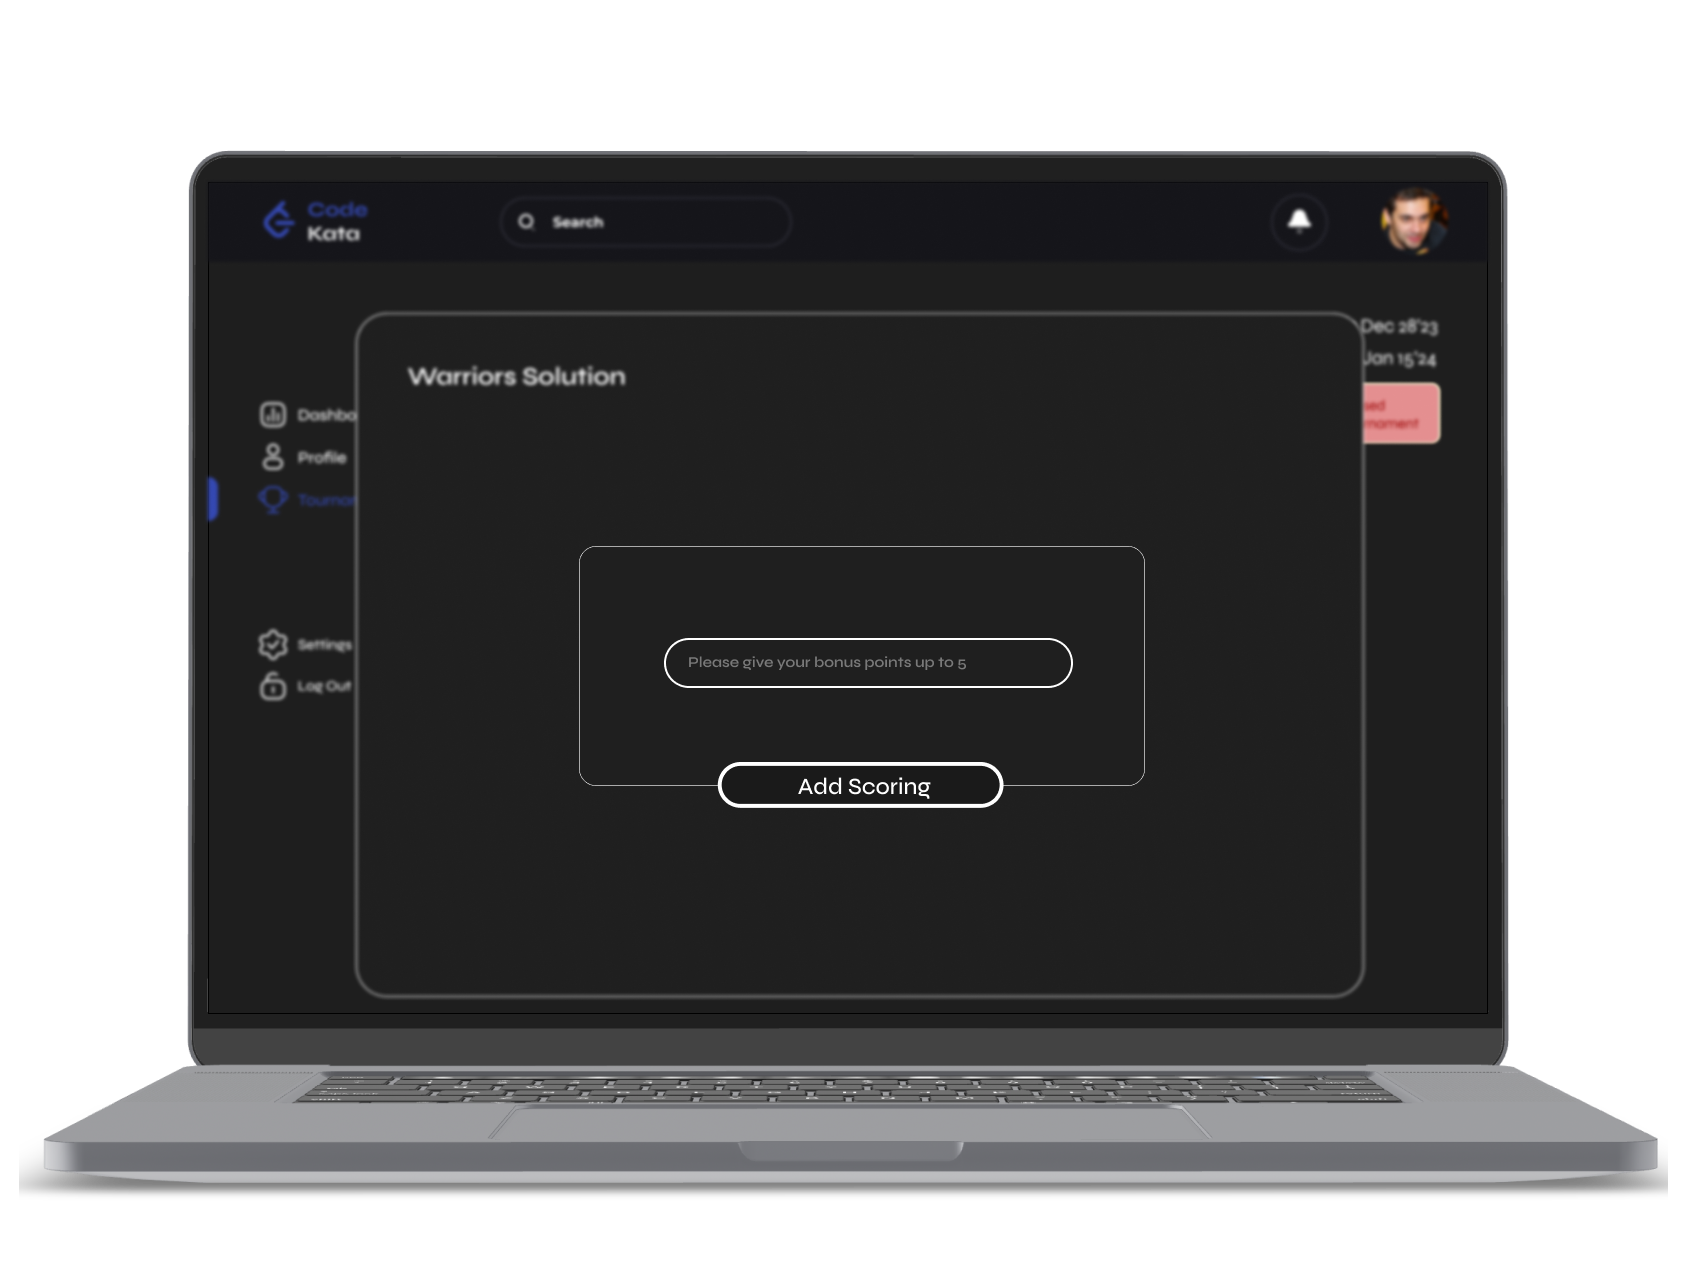
\includegraphics[scale=0.13]{Images/ui-ux/educator_team/educator_team_3.png}
% 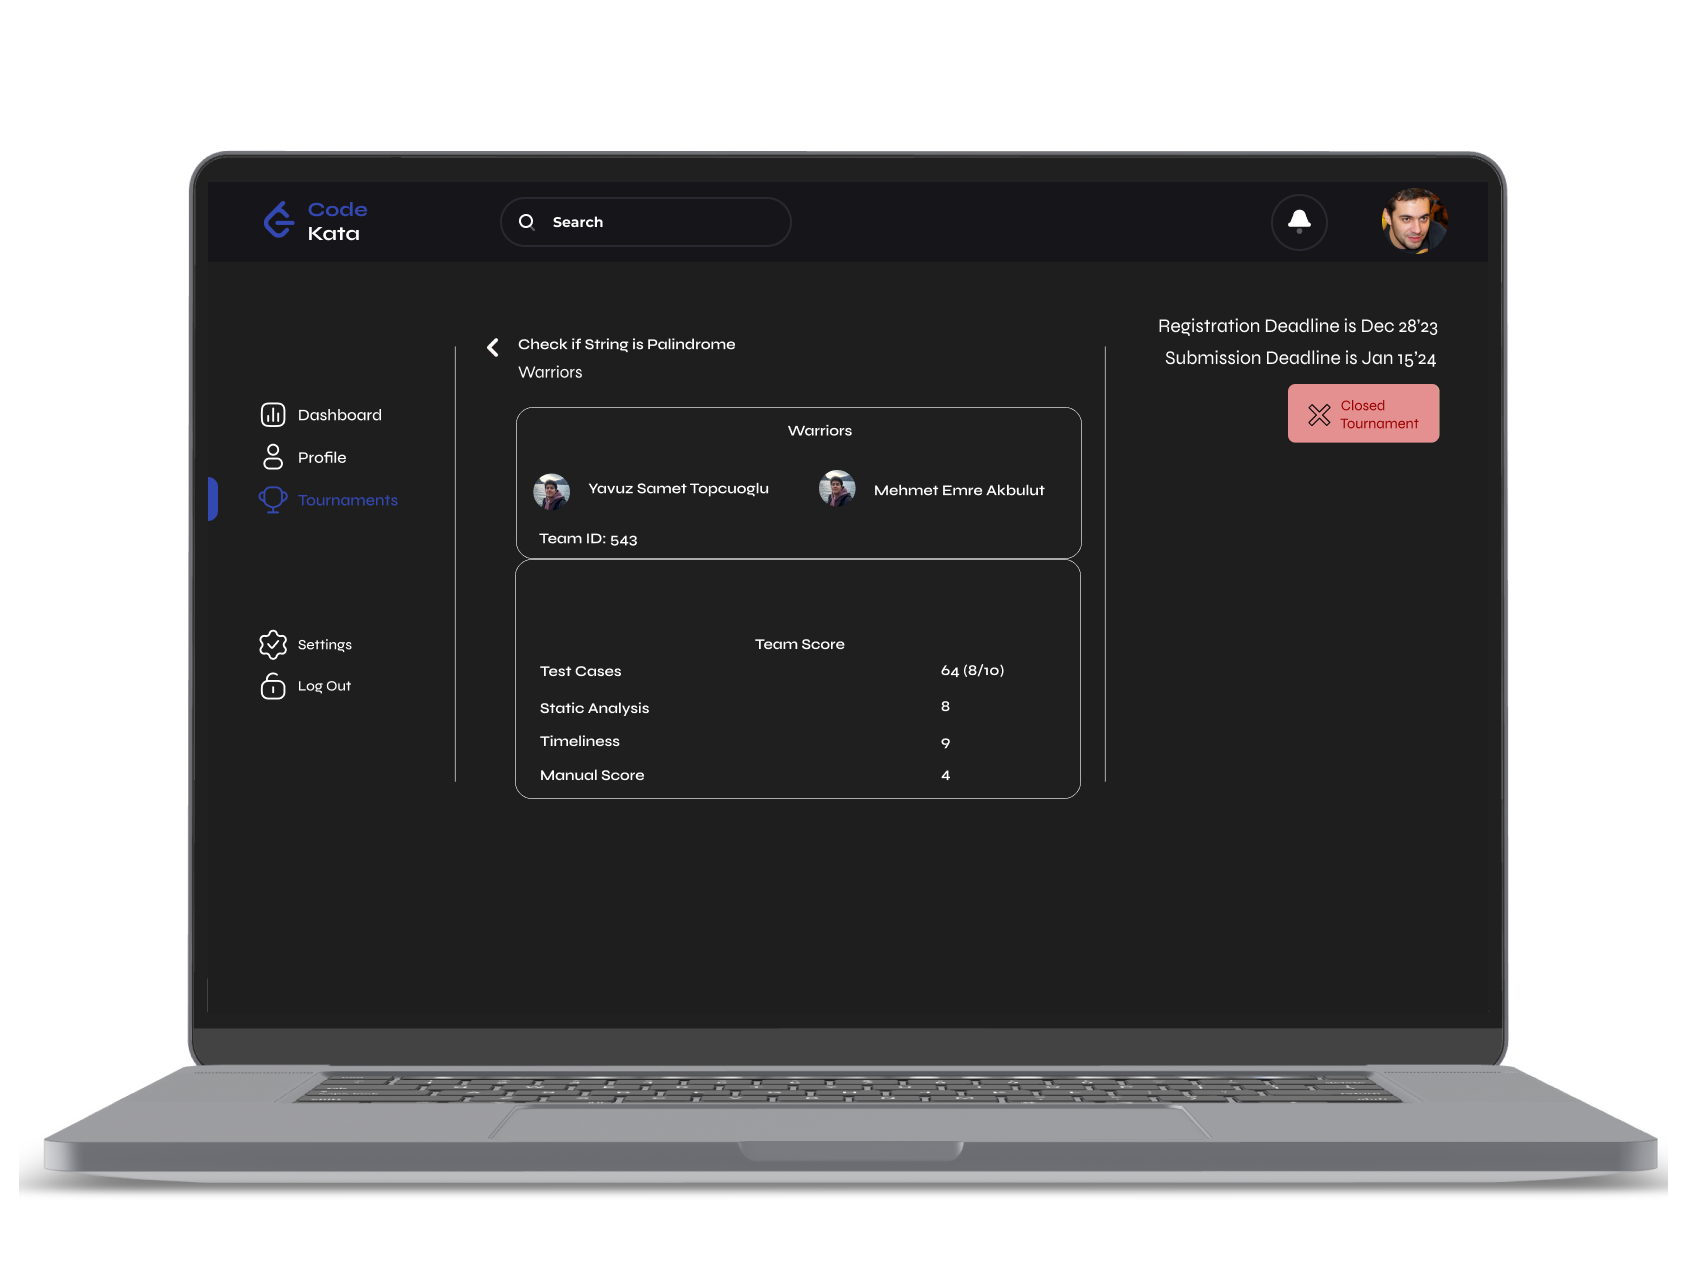
\includegraphics[scale=0.13]{Images/ui-ux/educator_team/educator_team_4.png}
%         (a) Educator, Team and Manual Scoring
% \end{center}
% \begin{center}
% 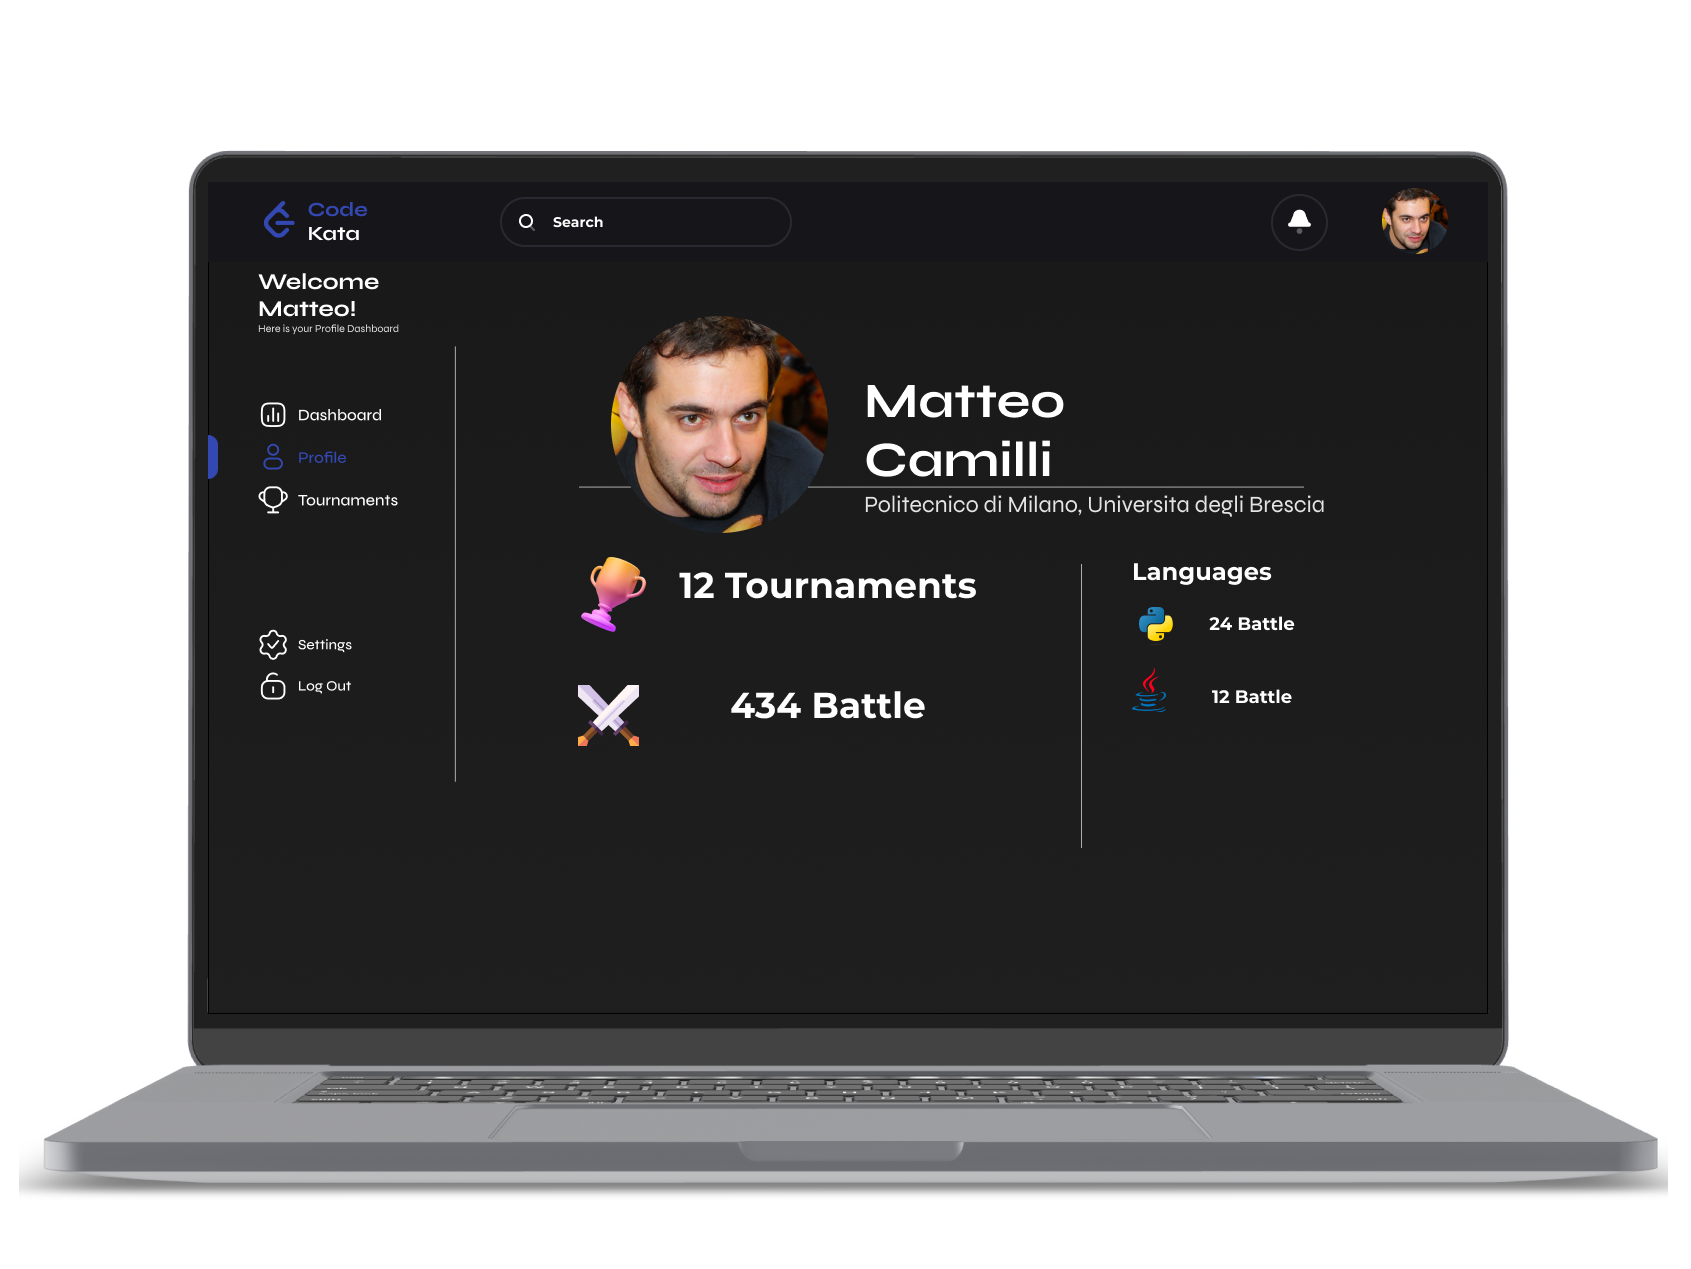
\includegraphics[scale=0.13]{Images/ui-ux/educator_profile_settings/educator_profile.png}
% 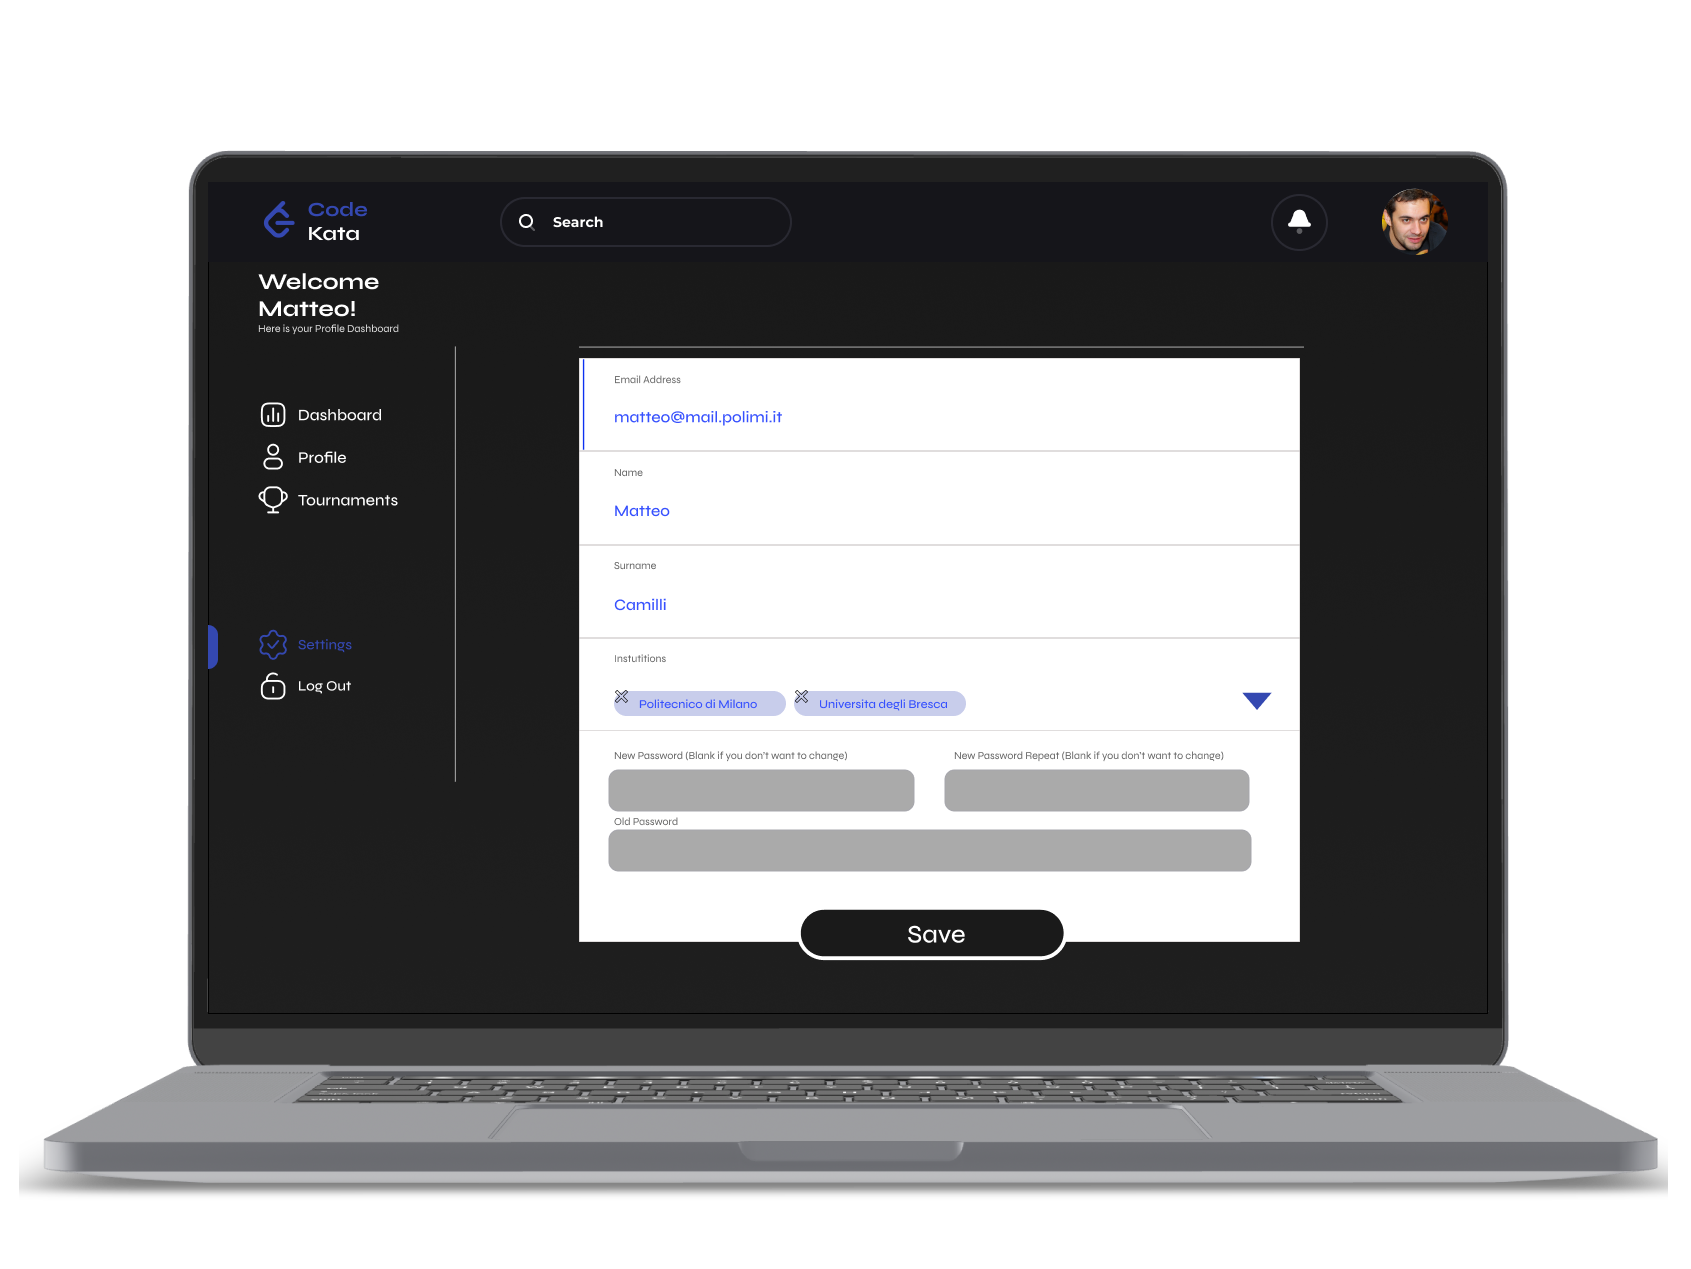
\includegraphics[scale=0.13]{Images/ui-ux/educator_profile_settings/educator_settings.png}
%         (a) Educator Profile and Settings
% \end{center}
\newpage
    
\subsubsection{Hardware Interfaces}
The CodeKataBattle platform operates entirely through web interfaces, eliminating the need for specialized hardware interfaces. Users can access the platform using standard web-enabled devices, such as computers, tablets, and smartphones. The platform is designed to function within a web browser, requiring no specific hardware beyond a device capable of running a modern browser and accessing the internet. This approach ensures broad accessibility without necessitating particular hardware configurations, making the platform versatile and user-friendly across various hardware setups. However, for optimal experience, at least 2GB of RAM and a minimum of 1GB of free space are recommended for browser caching and temporary files.

\subsubsection{Software Interfaces}
Our platform CKB interfaces with various software systems:

\begin{itemize}
    \item \textbf{Web Browsers:} Platform operates on web browsers. For universal access and easy use, it is compatible with major browsers like Chrome, Edge, Safari, Opera, and Firefox.

    \item \textbf{GitHub API:} Integrated for creating coding repositories and managing code \textit{submission} processes.

    \item \textbf{Sandboxing:} To create an isolated testing environment, our Sandbox Manager will utilise Docker.

    \item \textbf{Static Analysis Tool:} SonarQube API will be integrated for scoring the quality aspect of the code with static analysis. 

    \item \textbf{Database Technology:} Platform uses databases such as PostgreSQL.

    \item \textbf{Hosting:} Our platform uses Amazon Web Services EC2 for web server and database hosting.

    \item \textbf{Cloud File Storage:} The files will be stored using Amazon S3 services.

    \item \textbf{Email Service:} Amazon Simple Email Service SES will be used to send automated email notifications.
\end{itemize}

\subsubsection{Communication Interfaces}
Our platform utilises various communication systems:

\begin{itemize}
    \item \textbf{HTTPS:} For secure connection over the internet.

    \item \textbf{RESTful APIs:} We have RESTful APIs to communicate with the requests coming from GitHub Actions and the web application.

    \item \textbf{SMTP:} It is used to manage to send automated emails.
\end{itemize}

\subsection{Functional Requirements}
\subsubsection{Use Case Diagrams}
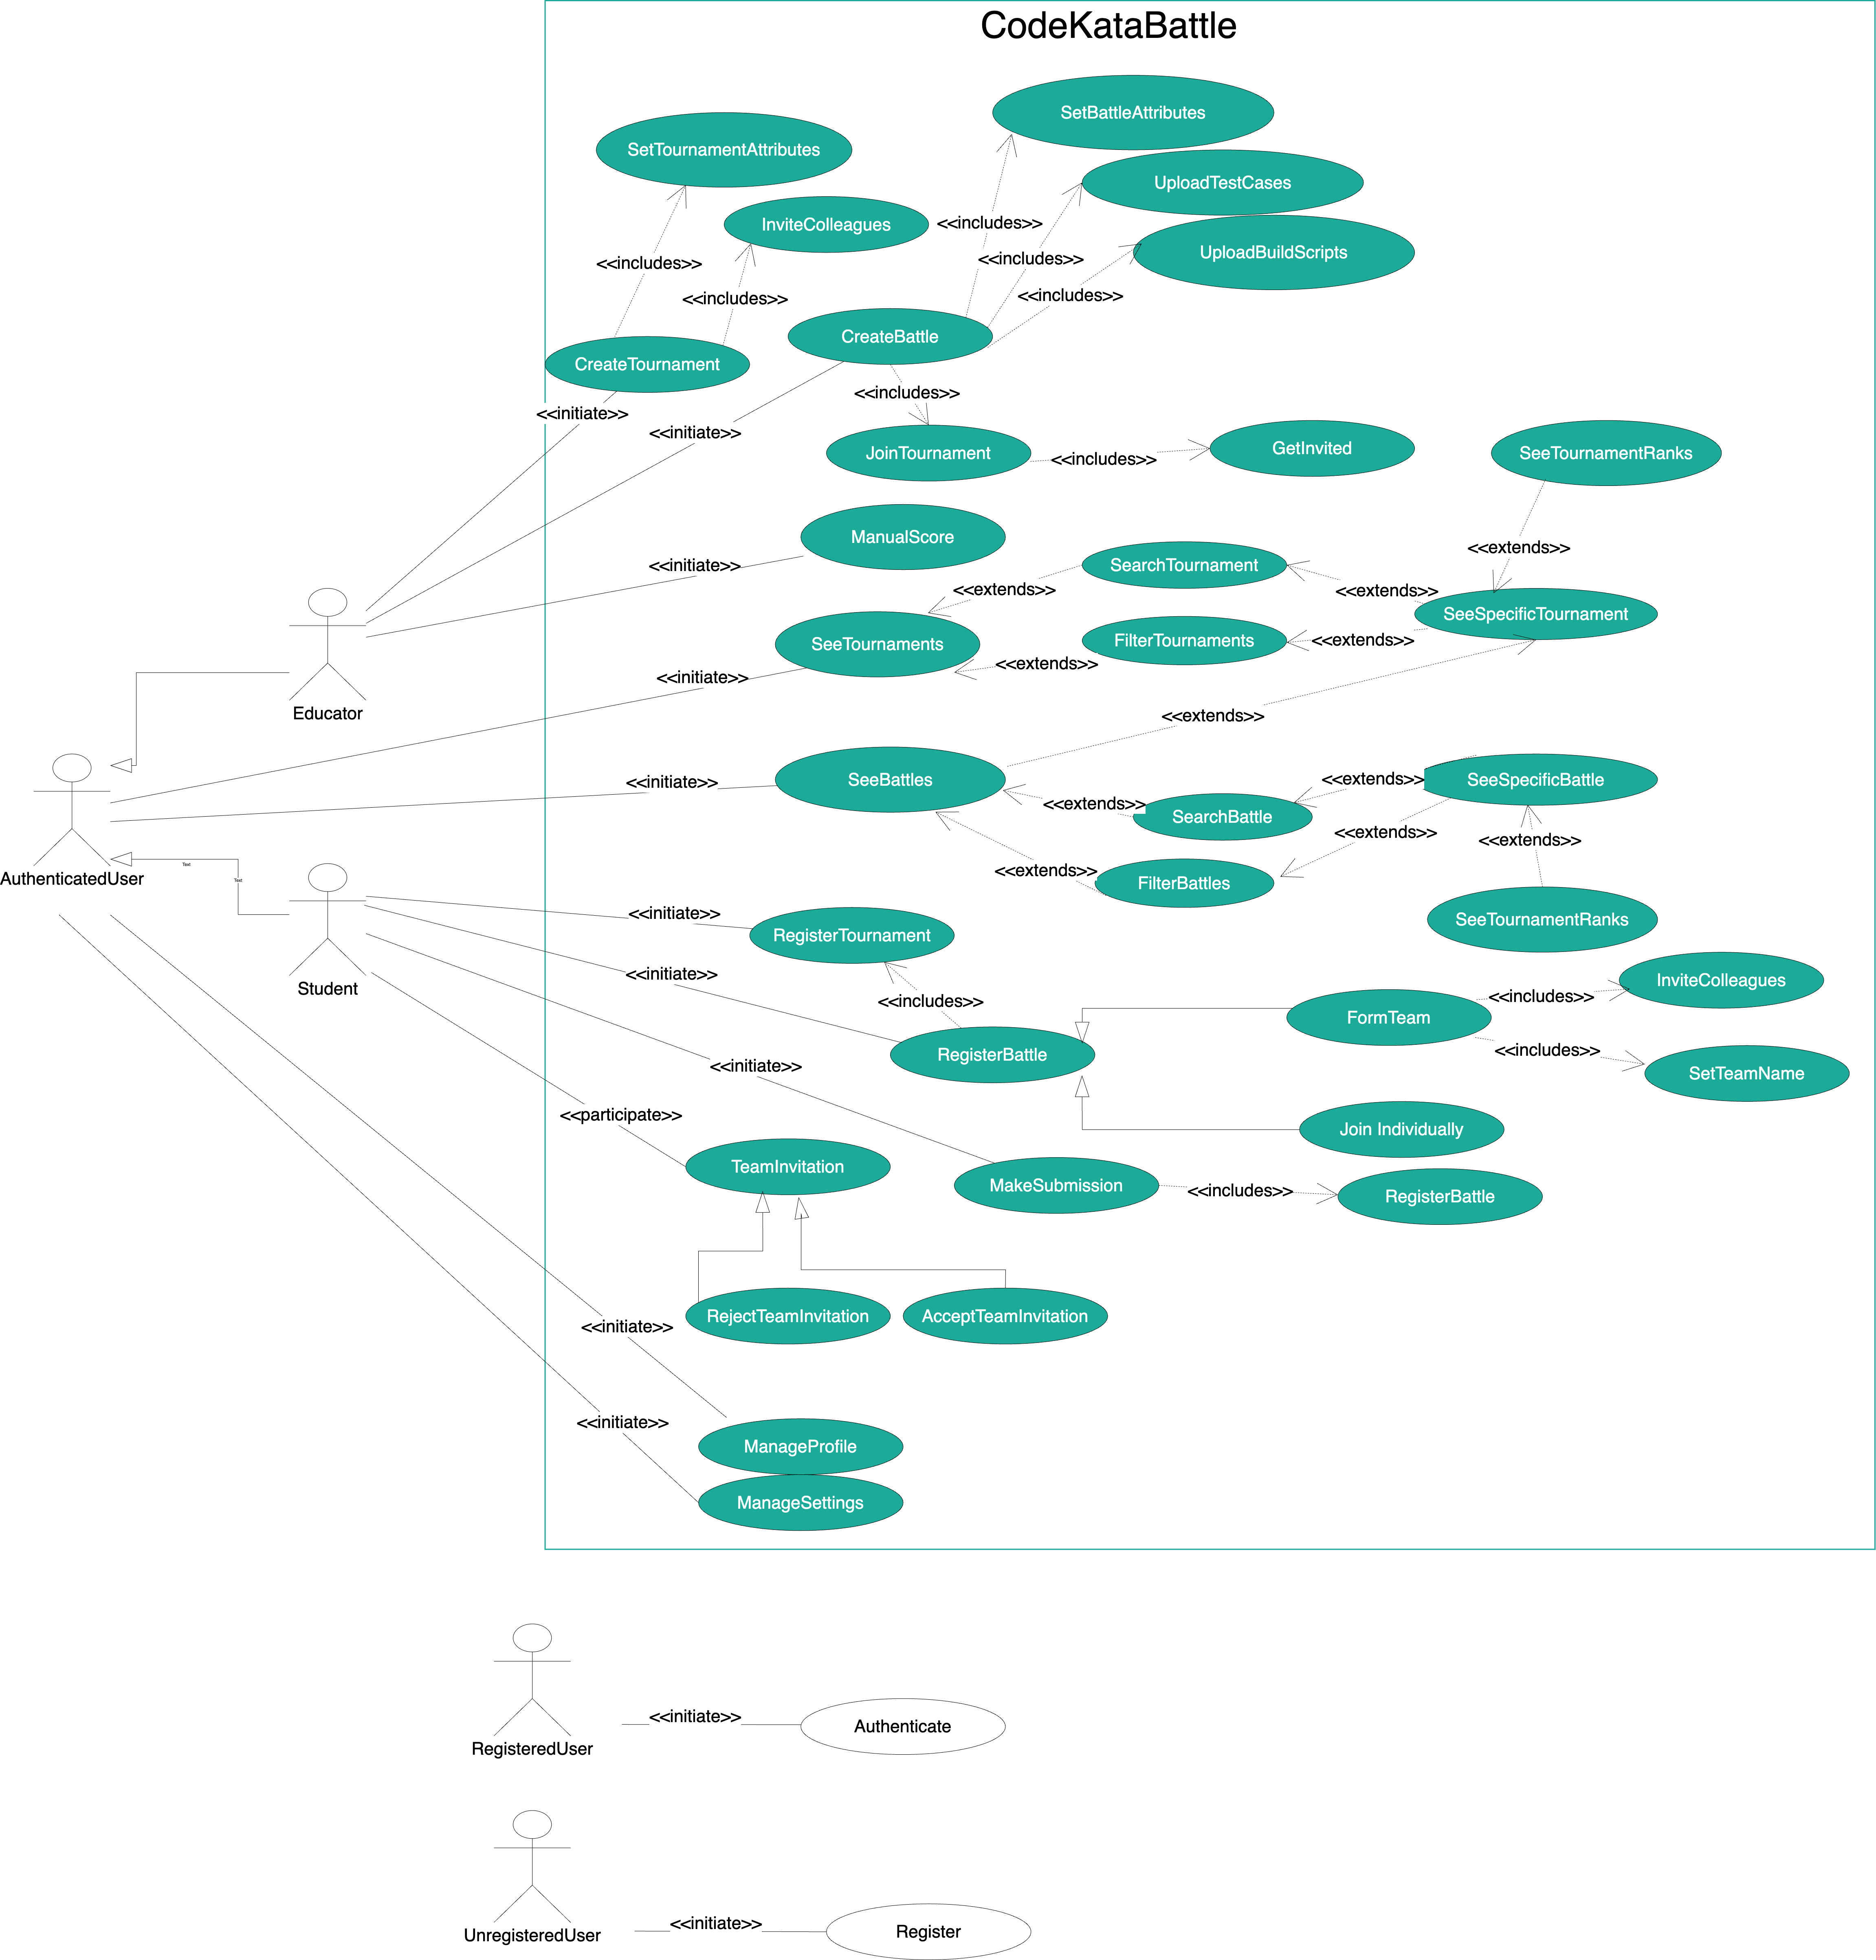
\includegraphics[scale=0.27]{Images/use_case_diagrams.drawio.png}
\newpage
\quad Unregistered User Actor has been used to illustrate the Registration Use Case. Similarly, the Registered User Actor has been used to show the Authentication Use Case. Other user actors are assumed to be registered and authenticated.

\quad Our system is composed of two main user types: Student and Educator. In the use case diagram, we showed common use cases with the Authenticated User actor. Authenticated User, simply every user registered to the platform, can view Tournaments, Battles, and their rankings with different filters and search options. Moreover, Registered User has the capability of viewing their profile and editing settings.

\quad Use case related Educator and Student Actors summarizes the goal of these users in the system.

\quad Invitee Student and Invitee Educator Actors are used to demonstrate use cases for tournament(for educators) and team(for students) invitations.

\quad GitHub System Boundary contains use cases about code submission with the participation of GitHub API Actor.



